\documentclass{llncs}
%\smartqed  % flush right qed marks, e.g. at end of proof
\usepackage{stmaryrd}
\usepackage{citesort} % removed because it clashes with the hyperref package
\usepackage{bussproofs}
\usepackage{turnstile}
\usepackage{amssymb}
\usepackage{latexsym}
\setcounter{tocdepth}{3}
\usepackage{graphicx}
\usepackage{url}
\usepackage{amsmath}
\usepackage{listings}
\usepackage{subfig}
\usepackage{pgf}
\usepackage{tikz}
\usetikzlibrary{arrows,shapes,snakes,automata,backgrounds,petri}
\usepackage[latin1]{inputenc}
\usepackage{float}
\usepackage{amssymb}
\usepackage{wrapfig}
\usepackage{lscape}
\usepackage[counterclockwise]{rotating}
%\usepackage{hyperref}

\usepackage{ifthen}
\usepackage{amssymb}
\newboolean{showcomments}
\setboolean{showcomments}{true}
\ifthenelse{\boolean{showcomments}}
  {\newcommand{\mynote}[2]{
    \fbox{\bfseries\sffamily\scriptsize#1}
    {\small$\blacktriangleright$\textsf{\emph{#2}}$\blacktriangleleft$}
   }
  }
  {\newcommand{\mynote}[2]{}
  }
\newcommand\martin[1]{\mynote{Martin}{#1}}
\newcommand\richard[1]{\mynote{Richard}{#1}}

\newcommand{\NOVSPACEPARAGRAPH}[1]{\NI\textbf{\emph{#1}.}}
\newcommand{\PARAGRAPH}[1]{\vspace{2mm}\NOVSPACEPARAGRAPH{#1}}
\newcommand{\NI}{\noindent}
\newcommand{\LEQ}{\sqsubseteq}
\newcommand{\BISIM}{\sim}
\newcommand{\BIGLUB}{\bigsqcup}
\newenvironment{FIGURE}{\begin{figure}[h]\rule{\linewidth}{0.5pt}
 %\vspace{3.2mm}
}{\rule{\linewidth}{0.5pt}\end{figure}}
\newenvironment{RULES}{\[\begin{array}{c}}{\end{array}\]}
\newenvironment{GRAMMAR}{\[\begin{array}{lcl}}{\end{array}\]}
\newcommand{\VERTICAL}{\  \mid\hspace{-3.0pt}\mid \ }
\newcommand{\infer}[2]{\frac{\displaystyle{ #1 }}{\displaystyle{ #2 }}}
\newcommand{\ZEROPREMISERULE}[1]{\infer{-}{#1}}
\newcommand{\ONEPREMISERULE}[2]{\infer{#1}{#2}}
\newcommand{\TWOPREMISERULE}[3]{\infer{#1 \quad #2}{#3}}
\newcommand{\THREEPREMISERULE}[4]{\infer{#1 \quad #2 \quad #3}{#4}}
\newcommand{\FOURPREMISERULE}[5]{\infer{#1 \quad #2 \quad #3 \quad #4}{#5}}
\newcommand{\SIXPREMISERULE}[7]{\infer{#1 \quad #2 \quad #3 \quad #4 \quad #5 \quad #6}{#7}}
\newcommand{\RULENAME}[1]{\textsc{#1}}
\newcommand{\SMALLRULENAME}[1]{\textsc{\tiny #1}}
\newcommand{\ZEROPREMISERULENAMEDRIGHT}[2]{\ZEROPREMISERULE{#1}\,\SMALLRULENAME{#2}}
\newcommand{\ONEPREMISERULENAMEDRIGHT}[3]{\ONEPREMISERULE{#1}{#2}\,\SMALLRULENAME{#3}}
\newcommand{\TWOPREMISERULENAMEDRIGHT}[4]{\TWOPREMISERULE{#1}{#2}{#3}\,\SMALLRULENAME{#4}}
\newcommand{\THREEPREMISERULENAMEDRIGHT}[5]{\THREEPREMISERULE{#1}{#2}{#3}{#4}\,\SMALLRULENAME{#5}}
\newcommand{\FOURPREMISERULENAMEDRIGHT}[6]{\FOURPREMISERULE{#1}{#2}{#3}{#4}{#5}\,\SMALLRULENAME{#6}}
\newcommand{\ZEROPREMISERULENAMEDLEFT}[2]{\SMALLRULENAME{#2}\,\ZEROPREMISERULE{#1}}
\newcommand{\ONEPREMISERULENAMEDLEFT}[3]{\SMALLRULENAME{#3}\,\ONEPREMISERULE{#1}{#2}}
\newcommand{\TWOPREMISERULENAMEDLEFT}[4]{\SMALLRULENAME{#4}\,\TWOPREMISERULE{#1}{#2}{#3}}
\newcommand{\THREEPREMISERULENAMEDLEFT}[5]{\SMALLRULENAME{#5}\,\THREEPREMISERULE{#1}{#2}{#3}{#4}}
\newcommand{\FOURPREMISERULENAMEDLEFT}[6]{\SMALLRULENAME{#6}\,\FOURPREMISERULE{#1}{#2}{#3}{#4}{#5}}

\newcommand{\MAY}[2]{\langle #1 \rangle #2}
\newcommand{\NEG}[1]{\mathsf{neg}(#1)}
\newcommand{\AND}{\land}
\newcommand{\INC}[1]{\mathsf{Inc}(#1)}

\newcommand{\CAL}[1]{\mathcal{#1}}
\newcommand{\FRAK}[1]{\mathfrak{#1}}
\newcommand{\SEMB}[1]{\lbrack\!\lbrack #1 \rbrack\!\rbrack}
\newcommand{\STATE}{\mathsf{State}}
\newcommand{\SYMBOL}{\mathsf{Symbol}}
\newcommand{\DEFEQ}{\stackrel{\text{\emph{def}}}{=}}
\newcommand{\TRUTH}{\LOGIC{T}}
\newcommand{\TRUE}{\LOGIC{t}}
\newcommand{\LOGIC}[1]{\mathsf{#1}}
\newcommand{\MMM}{\frak{M}}
\newcommand{\SSS}{\CAL{S}}
\newcommand{\IMPLIES}{\supset}
\newcommand{\RED}{\rightarrow}
\newcommand{\RESTRICT}[2]{\mathsf{Restrict}_{#1}(#2)}
\newcommand{\ARROW}[2]{\mathsf{Arrow}(#1, #2)}
\newcommand{\LLL}{\mathcal{L}}
\newcommand{\RRR}{\mathcal{R}}
\newcommand{\TRANS}[1]{\stackrel{#1}{\longrightarrow}}

\newcommand{\QUOTATION}[1]{
\hfill
\hspace{58mm}
\begin{minipage}{60mm}\tiny #1\end{minipage}
}

\lstnewenvironment{code}
    {\lstset{}%
      \csname lst@SetFirstLabel\endcsname}
    {\csname lst@SaveFirstLabel\endcsname}
    \lstset{
      basicstyle=\small\ttfamily,
      flexiblecolumns=false,
      basewidth={0.5em,0.45em},
      literate={+}{{$+$}}1 {/}{{$/$}}1 {*}{{$*$}}1 {=}{{$=$}}1
               {>}{{$>$}}1 {<}{{$<$}}1 {\\}{{$\lambda$}}1
               {\\\\}{{\char`\\\char`\\}}1
               {->}{{$\rightarrow$}}2 {>=}{{$\geq$}}2 {<-}{{$\leftarrow$}}2
               {<=}{{$\leq$}}2 {=>}{{$\Rightarrow$}}2 
               {\ .}{{$\bigcirc$}}2 {\ .\ }{{$\bigcirc$}}2
               {>>}{{>>}}2 {>>=}{{>>=}}2
               {|}{{$\mid$}}1               
    }

\newtheorem{mycase}{Case}
\newtheorem{subcase}{Case}
\numberwithin{subcase}{mycase}


% Dot
\def\fDot {\ast}
% Bang
\def\fBang {\ ! \ }
% Or
\def\fOr {\ | \ }

% Turnstiles with subscripts
\def\judgeX {\sststile{\mathrm{X}}{}}
\def\judgeY {\sststile{\mathrm{Y}}{}}
%\def\judge {\sststile{\mathrm{}}{}}

\newcommand{\judge}{\vdash}

\EnableBpAbbreviations


\begin{document}

\title {Cathoristic logic}
\subtitle{A logic for capturing inferences between atomic sentences}
\titlerunning{Cathoristic logic}
\author{Richard Prideaux Evans\inst{1} \and  Martin Berger\inst{2}}
\authorrunning{Prideaux Evans and Berger}
\institute {Richard Prideaux Evans, Imperial College, \email{richardevans@google.com}
  \and
 Martin Berger, University of Sussex, \email{M.F.Berger@sussex.ac.uk}.}

\bibliographystyle{abbrv} 
\maketitle

\begin{abstract}
[To do.]
\end{abstract}


\section{Introduction}\label{introduction}

Natural language is full of mutually-exclusive alternatives.
If Pierre is the current king of France, then nobody else can concurrently fill that role.
A traffic light can be green, amber or red - but it cannot be more than one at a time.
Mutual exclusion is a natural and ubiquitous concept.

Predicate logic \emph{can} represent mutually exclusive alternatives, of course.
To say that Pierre is the \emph{only} king of France, we can write, following Russell:
\[
king(france, pierre) \land \forall X . king(france, X) \rightarrow X = pierre
\]
To say that a particular traffic light, $t$, is red - and red is its \emph{only} colour - we could write:
\[
colour(t, red) \land \forall X . colour(t, X) \rightarrow X = red
\]
In predicate logic, exclusion is a \emph{derived} concept, reduced to a combination of universal quantification and identity.
Predicate logic, in other words, uses relatively complex machinery to express a simple concept:
\begin{itemize}
\item Quantification is an expensive concept that comes with
      many rules governing its behaviour - such as the distinction
      between free and bound variables\footnote{As of 2014 there is a substantial amount
      of ongoing research regarding good formalisations of handling
      free/bound variables, see e.g.~nominal approaches to
      logic \cite{PittsAM:newaas,PittsAM:nomsetnasics}. The problem
      was put in focus in recent years with the rise in interest in the
      computational cost of syntax manipulation in languages with
      binders.}. The costs of quantification have to be
      borne every time one uses exclusion, \emph{even though exclusion does
      not, prima facie, appear to have anything to do with the
      free/bound variable distinction}.
\item The identity relation is also an expensive piece of machinery. In first order predicate logic, identity is a special-case relation which requires an infinite axiom schema (the Indiscernibility of Identicals) to capture its unique properties.
\end{itemize}

This paper introduces an alternative logic, \ELFULL{}, in which exclusion is expressed \emph{directly}, as a first-class concept - rather than defined in terms of relatively complex machinery.
\ELFULL{} is the simplest logic we could find that expresses exclusion directly. 
Exclusion and conjunction are the \emph{only} logical operators. 
There is no negation, disjunction or implication.
Because of its extreme simplicity, it has a linear-time decision procedure.

\ELFULL{} is a multi-modal logic, a variant of Hennessy-Milner Logic, that replaces negation with a different logical connective:
\[
   !A
\]
called \emph{just} $A$, or \emph{tantum} $A$.
Here, $A$ is a finite set of alternatives that exhaust all
possibilities. 
For example:
\begin{eqnarray*}
\fBang \{green, amber, red\}
\end{eqnarray*}
Any statement of a fact that exceeds what tantum $A$ allows is necessarily false:
\[
   !\{green, amber, red\} \AND \MAY{blue}
\]
is necessarily false.
If the only available options are green, amber, or red, then blue is not an available option.

Now to say that Pierre is the only king of France, we write:
\[
\MAY{king}\MAY{france}(\MAY{pierre} \land \fBang \{pierre\})
\]
Note that \ELFULL{}'s representation of exclusion involves no universal quantifier and no identity relation.
It is a purely propositional representation of exclusion.

To say that the traffic light is currently red, and \emph{red is its only colour}, we write:
\[
\MAY{t} \MAY{colour} (\MAY{red} \land !\{red\})
\]
This is markedly simpler (both in terms of representation length and computational complexity) than the representation in predicate logic:
\[
colour(t, red) \land \forall X . colour(t, X) \rightarrow X = red
\]
To summarise the argument we shall be presenting:
\begin{itemize}
\item
Every fundamental logical concept needs a logic in which it can be expressed naturally (ergonomically)
\item
Exclusion is a fundamental logical concept
\item
First order logic does not express exclusion naturally\footnote{We will precisify this claim in later sections by showing that (i) first order logic's representation of exclusion is significantly longer in terms of formula length than \ELFULL{}'s (see Section \ref{incompatiblepredicatesinfol}); and (ii) logic programs in \ELFULL{} can be optimised to run significantly faster than their equivalent in FOL (see Section \ref{optimizingpreconditions}).}
\item
\ELFULL{} expresses exclusion directly
\item
Because it expresses exclusion directly, it has various unusual features. 
Because it eschews the complexifying logical operators $\neg, \lor$ and $\Rightarrow$, it has a \emph{linear-time} decision procedure. 
Nevertheless, despite its simplicity, it is sufficiently expressive to satisfy both:
\begin{itemize}
\item
The Hennessy-Milner theorem (Theorem \ref{theorem:completeLattice})
\item
Brandom's Incompatibility Semantics property (Theorem \ref{incompatibilitytheorem})
\end{itemize}
\end{itemize}
In the next subsections, we shall:
\begin{itemize}
\item
Strengthen the claim that exclusion is a fundamental logical concept, by arguing that exclusion is conceptually prior to negation
\item
Broaden the claim that exclusion is a fundamental logical concept, by adding other sorts of intra-sentential logical concepts that predicate logic cannot handle (naturally, or at all). These other forms of intra-sentential inferential relations can all be handled naturally in \ELFULL{}.
\end{itemize}

\subsection{Exclusion as a Fundamental Logical Concept, Conceptually Prior to Negation}

Consider the sentences:
\begin{enumerate}

\item ``Jack is male'' is incompatible with ``Jack is female''
\item For every person $x$, if $x$ is male, then it is not the case that $x$ is female

\end{enumerate}

\NI The orthodox position is that (1) is true because of (2).  There
are \emph{general universally-quantified rules} describing which
predicates are incompatible, and these general rules explain why
particular sentence instances are incompatible.  We know (1) because
we know (2).

In \emph{Making It Explicit}\cite{brandom2}, Brandom proposes a reversal of this
orthodox direction of explanation.  He claims that we can understand
incompatible sentence pairs, like (1), even if we do not understand
universal quantification or negation.  \emph{Material incompatibility is
conceptually prior to logical negation.}

Imagine, to make this vivid, a primitive people speaking a
primordial language.  This language contains atomic sentences, but has
no ``complex'' logical connectives.  By ``complex'', I mean logical
connectives that, like disjunction, generate sentences which can be
satisfied in many different distinct ways.  Negation, disjunction,
implication, existential quantification all create formulae that can
be satisfied in many different ways (but conjunction does not). This condition will be
precisified in Section 2: a logic is ``simple'' if the set of
satisfying models of every sentence has a unique least upper
bound. Disjunction fails to be simple because there are two equally
simple models of $\phi \lor \psi$. Similarly, negation fails to be simple
because there are two equally simple models of $\neg (\phi \land
\psi)$. Conjunction is the \emph{only} connective of propositional logic that is simple,
according to this criterion.

Imagine, then, a primitive people speaking a simple language of
atomic sentences - a language containing no operators for generating
sentences that can be satisfied in different ways.  These people
recognise when atomic sentences are incompatible, and can see that one
sentence entails another - but they have no way of saying explicitly
that these sentences have these properties.  Their behaviour
outreaches their ability to articulate it.  Over time, these people
may advance to a more sophisticated language in which
incompatibilities and entailments can be made explicit (using the
negation and entailment operators respectively) - but this is a later
(and optional) development. The speakers of the core primordial
language understand incompatibility relations between atomic
sentences, but use no complex logical connectives.

If this picture is coherent, then material incompatibility - exclusion - is conceptually independent of logical negation.
We do not need negation to make sense of exclusion.

Now imagine a variation of our primitive language in which no sentences are ever treated as incompatible.
The native speakers never disagree, back down, retract their claims, or justify them. They just make assertions.
Without an understanding of incompatibility, and the variety of behaviour that it engenders, we submit (following Brandom) that there is insufficient richness in the linguistic practice for their sounds to count as assertions.
Without exclusion, their sounds are just \emph{barks}.
If this further claim is also accepted, then material incompatibility - exclusion - is not just conceptually \emph{independent} of logical negation, but is conceptually \emph{prior} to it.


\subsection{Intra-Sentential Logical Operators}

The core claim of this paper is that \ELFULL{} is an ergonomic logic for describing the exclusion relation.
Now exclusion is an inferential relation between \emph{atomic sentences}. 
In this subsection, we shall describe \emph{other} inferential relations between atomic sentences - inferential relations that predicate logic cannot articulate, but that \ELFULL{} is able to handle.

The \emph{atomic sentences} of a natural language can be
characterised as the sentences which do not contain any other
sentences as constituent parts\footnote{Compare Russell \cite{russell}
  p.117: ``A sentence is of atomic form when it contains no logical
  words and no subordinate sentence''. We use a broader notion of
  atomicity by focusing solely on whether or not it contains a
  subordinate sentence, allowing logical words such as ``and'' as long
  as they are conjoining noun-phrases and not sentences.}.  According
to this criterion, the following are atomic:

\begin{itemize}

\item Jack is male
\item Jack loves Jill
\end{itemize}

\NI The following is not atomic:

\begin{quote}
  Jack is male and Jill is female
\end{quote}

\NI because it contains the complete sentence ``Jack is male'' as a
syntactic constituent.  Note that, according to this criterion, the
following \emph{is} atomic, despite using ``and'' :

\begin{quote}
  Jack loves Jill and Joan
\end{quote}

\NI Here, ``Jack loves Jill'' is not a syntactic constituent since
``and'' is used to conjoin \emph{noun-phrases}, not sentences.

There are many types of inferential relations between atomic
sentences of a natural language.  For example:

\begin{itemize}

\item ``Jack is male'' is incompatible with ``Jack is female''
\item ``Jack loves Jill'' implies ``Jack loves''
\item ``Jack walks slowly'' implies ``Jack walks''
\item ``Jack loves Jill and Joan'' implies ``Jack loves Jill''
\item ``Jack is wet and cold'' implies ``Jack is cold''

\end{itemize}

\NI Some of these inferential relations are \emph{exclusion}
relations (two sentences cannot both be true) while others are
\emph{entailment} relations (if one sentence is true, the other must
also be true).  The main question this paper seeks to answer is:
\emph{what is the simplest logic that can capture these inferential
  relations?}

\subsection{Wittgenstein's vision of a logic of elementary propositions}

\NI In the \emph{Tractatus} \cite{wittgenstein-tractatus}, Wittgenstein
claimed that the world is a set of atomic sentences in an idealized
logical language.  Each atomic sentence was supposed to be
\emph{logically independent} of every other, so that they could be
combined together in every possible permutation, without worrying
about their mutual compatibility.

But already there were doubts and problem cases.  He was aware that
certain sorts of statements seemed atomic, but did not seem logically
independent:

\begin{quote}
  For two colours, e.g., to be at one place in the visual field is
  impossible, and indeed logically impossible, for it is excluded by
  the logical structure of colour. (6.3751)
\end{quote}

\NI At the time he was writing the Tractatus, he hoped that further
analysis would reveal that these statements were not really atomic.

But in the \emph{Philosophical Remarks} \cite{wittgenstein-remarks}, he
renounced the thesis of the logical independence of atomic
propositions.  In \S 76, talking about incompatible colour predicates,
he writes:

\begin{quote}
  That makes it look as if \emph{a construction might be possible
    within the elementary proposition}. That is to say, as if there
  were a construction in logic which didn't work by means of truth
  functions.  What's more, it also seems that these constructions have
  an effect on one proposition's following logically from another.
  For, if different degrees exclude one another it follows from the
  presence of one that the other is not present.  In that case,
  \emph{two elementary propositions can contradict one another}.
\end{quote}

\NI Here, he is clearly imagining a logical language in which there
are incompatibilities between atomic propositions. In \S 82:

\begin{quote}
  This is how it is, what I said in the Tractatus doesn't exhaust the
  grammatical rules for 'and', 'not', 'or', etc; \emph{there are rules
    for the truth functions which also deal with the elementary part
    of the proposition}.  The fact that one measurement is right
  \emph{automatically} excludes all others.
\end{quote}

\NI But Wittgenstein does not, unfortunately, show us what this
language would look like.  In this paper, a new modal logic is
introduced to articulate Wittgenstein's vision.  \ELFULL{} is the simplest logic we could find that handles the various types of inferences between elementary propositions.

\subsection{Outline}
The rest of this paper is organised as follows:
\begin{itemize}
\item
We describe the syntax and semantics of \ELFULL{}
\item
We provide inference rules, and prove soundness, completeness and compactness
\item
We describe a \emph{linear-time} decision procedure
\item
We prove a version of the Hennessy-Milner theorem
\item
We show that \ELFULL{} satisfies Brandom's Incompatibility Semantics requirement
\item
We show how \ELFULL{} has been used as an ergonomic knowledge-representation language in an industrial application
\end{itemize}

\subsubsection{Discussion: Precisifying the Negation. }

\NI If someone asserts that, say, Jack does not support Manchester United,
we have so far said very little.  Until we know the \emph{range of
  football teams} he could support, we don't know what the negation
amounts to.  Until we have some more determinate information about the
range of possible choices, there are an \emph{indefinite} number of
ways in which this could be true.  But if we knew that the only
possible teams Jack could support are Manchester United, Arsenal or
Chelsea, then suddenly our negation has some determinate content.
SNEL captures this intuition.  Once a negated formula has been
precisified by specifying the range of allowable options (via the $!$
operator), the negated claim can be made precise, and the law of
excluded middle can be proven.

\subsubsection{Discussion: Negation as Infinitary Disjunction. }
As is well known the existential quantifier of Predicate Logic can be translated into an infinitary disjunction of propositions in Propositional Logic.

Analogously, given an infinite set $S$ of symbols, the
negation of propositional logic can be translated into an infinitary
disjunction of formulae in SNEL.\martin{doesn't this argument also work for a finite
set $S$?}


\subsection{Introduction TODOs}

\begin{itemize}
\item Consider expressing ``Pierre is either male or female'' in
  propositional logic, without quantifiers: $sex(pierre, male) \lor
  sex(pierre, female) \land \neg (sex(pierre, male) \land sex(pierre,
  female))$.
\item
Consider placing the point (currently in Related Work, Brandom's
Incompatibility Semantics) - that $\neg p$ is the least information
claim that is incompatible with $p$ - into the section on Exclusion
being Conceptually prior to Negation.

\item Integrate the two section above on negation
\end{itemize}

\section{Mathematical preliminaries}\label{preliminaries}

\NI This section briefly surveys the mathematical background of our
paper.  A fuller account of order-theory can be found in
\cite{DaveyBA:intlatao}.  Labelled transition systems are explored in
\cite{SassoneV:modcontac,HennessyM:Algtheop} and bisimulations in
\cite{SangiorgiD:intbisac}. Finally, \cite{EndertonHB:matinttl} is one
of many books on first-order logic.

\PARAGRAPH{Order-theory}
A \emph{preorder} is a pair $(S, \sqsubseteq)$ where $S$ is a set, and
$\sqsubseteq$ is a binary relation on $S$ that is reflexive and
transitive. Let $T \subseteq S$ and $x \in S$. We say $x$ is an
\emph{upper bound} of $T$ provided $t \sqsubseteq x$ for all $t \in
T$. If in addition $x \sqsubseteq y$ for all upper bounds $y$ of $T$,
we say that $x$ is the \emph{least} upper bound of $T$.  The set of
all least upper bounds of $T$ is denoted $\BIGLUB T$.  \emph{Lower
  bounds}, \emph{greatest lower bounds} and $\BIGGLB T$ are defined
mutatis mutandis.  A \emph{partial order} is a preorder $\sqsubseteq$
that is also anti-symmetric.  A partial order $(S, \sqsubseteq)$ is a
\emph{lattice} if every pair of elements in $S$ has a least upper and
a greatest lower bound.  A lattice is a \emph{bounded lattice} if it
has top and bottom elements $\top$ and $\bot$ such that for all $x \in
S$:
\[
x \sqcap \bot = \bot \nonumber \qquad
x \sqcup \bot = x \nonumber \qquad
x \sqcap \top = x \nonumber \qquad
x \sqcup \top = \top \nonumber.
\]

\NI If $(S, \sqsubseteq)$ is a preorder, we can turn it into a
partial-order by quotienting: let $a \simeq b$ iff $a \sqsubseteq b$
as well as $b \sqsubseteq a$. Clearly $\simeq$ is an equivalence. Let
$E$ be the set of all $\simeq$-equivalence classes of $S$. We get a
canonical partial order, denoted $\sqsubseteq_E$, on $E$ by setting:
$[a]_{\simeq} \sqsubseteq_E [b]_{\simeq}$ whenever $a \sqsubseteq
b$. If all relevant upper and lower bounds exist in $(S,
\sqsubseteq)$, then $(E, \sqsubseteq_E)$ becomes a bounded lattice by
setting
\[
   [x]_{\simeq} \sqcap [y]_{\simeq} = [ x \sqcap y ]_{\simeq}
       \quad
   [x]_{\simeq} \sqcup [y]_{\simeq} = [ x \sqcup y ]_{\simeq}
       \quad
   \bot_{E} = [\bot]_{\simeq}
       \quad
   \top_{E} = [\top]_{\simeq}.
\]


\PARAGRAPH{Transition systems}
Let $\Sigma$ be a set of \emph{actions}.  A \emph{labelled transition
  system over $\Sigma$} is a pair $(\mathcal{S}, \rightarrow)$ where
$\mathcal{S}$ is a set of \emph{states} and $\rightarrow \subseteq
\mathcal{S} \times \Sigma \times \mathcal{S}$ is the \emph{transition
  relation}.  We write $x \xrightarrow{a} y$ to abbreviate $(x,a,y)
\in \rightarrow$. We let $s, t, w, w', x, y, z, ...$ range over
states, $a, a', b, ...$ range over actions and $\LLL, \LLL', ...$
range over labelled transition systems. We usually speak of labelled
transition systems  when the set of actions is clear from the
context.  We say $\LLL$ is \emph{deterministic} if $x \TRANS{a} y$ and
$x \TRANS{a} z$ imply that $y = z$. Otherwise $\LLL$ is
\emph{non-deterministic}.  A labelled transition system is
\emph{finitely branching} if for each state $s$, the set $\{t\ |\ s
\TRANS{a} t\}$ is finite.

\PARAGRAPH{Simulations and bisimulations}
Given two labelled transition systems $\LLL_i = (S_i, \rightarrow_i)$
over $\Sigma$ for $i = 1, 2$, a \emph{simulation from $\LLL_1$ to
  $\LLL_2$} is a relation $\RRR \subseteq S_1 \times S_2$ such that
whenever $(s, s') \in \RRR$: if $s \TRANS{a} s'$ then there exists a
transition $t \TRANS{a} t'$ with $(t, t') \in \RRR$.  We write $s \SIM
t$ whenever $(s, t) \in \RRR$ for some simulation $\RRR$.  We say
$\RRR$ is a \emph{bisimulation between $\LLL_1$ and $\LLL_2$} if both,
$\RRR$ and $\RRR^{-1}$ are simulations. Here $\RRR^{-1} = \{(y,
x)\ |\ (x, y) \in \RRR\}$.  We say two states $s, s'$ are
\emph{bisimilar}, written $s \BISIM s'$ if there is a bisimulation
$\RRR$ with $(s, s') \in \RRR$.

\PARAGRAPH{First-order logic}
A \emph{many-sorted first-order signature} is specified by the
following data.  A non-empty set of \emph{sorts}, a set \emph{function
  symbols} with associated \emph{arities}, i.e.~non-empty list of
sorts $\#(f)$ for each function symbol $f$; a set of \emph{relation
  symbols} with associated \emph{arities}, i.e.~a list of sorts
$\#(R)$ for each relation symbol $R$; a set of \emph{constant symbols}
with associated \emph{arity}, i.e.~a sort $\#(c)$ for each constant
symbol $c$. We say a function symbol $f$ is \emph{$n$-ary} if $\#(f)$
has length $n+1$. Likewise, a relation symbol is \emph{$n$-ary} if
$\#(R)$ has length $n$.

Let $\SSS$ be a signature. An \emph{$\SSS$-model} $\CAL{M}$ is an
object with the following components.  For each sort $\sigma$ a set
$U_{\sigma}$ called \emph{universe} of sort $\sigma$.  The members of
$U_{\sigma}$ are called \emph{$\sigma$-elements} of $\CAL{M}$; an
element $c^\CAL{M}$ of $U_{\sigma}$ for each constant $c$ of sort
$\sigma$; a function $f^\CAL{M} : (U_{\sigma_1}\times \dots \times
U_{\sigma_n}) \rightarrow U_{\sigma}$ for each function symbol $f$ of
arity $(\sigma_1, ..., \sigma_n, \sigma)$; a relation $R^\CAL{M}
\subseteq U_{\sigma_1}\times \dots \times U_{\sigma_n}$ for each
relation symbol $R$ of arity $(\sigma_1, ..., \sigma_n)$.

Given an infinite set of variables for each sort $\sigma$, the
\emph{terms} and \emph{first-order formulae} for $\SSS$ are given by
the following grammar
\begin{GRAMMAR}
  t &\ ::=\ & x \VERTICAL c \VERTICAL f(t_1, ..., t_n) \\[1mm]
  \phi &::=& t = t' \VERTICAL R(t_1, ..., t_n) \VERTICAL \neg \phi \VERTICAL \phi \AND \psi \VERTICAL \forall x.A
\end{GRAMMAR}

\NI Here $x$ ranges over variables of all sorts, $c$ over constants,
$R$ over $n$-ary relational symbols and $f$ over $n$-ary function
symbols from $\SSS$.  Other logical constructs such as disjunction or
existential quantification are given by de Morgan duality, and truth
$\top$ is an abbreviation for $x = x$. If $\SSS$ has just a single
sort, we speak of \emph{single-sorted first-order logic} or just
\emph{first-order logic}. 

Given an $\SSS$-model $\CAL{M}$, an \emph{environment}, ranged over by
$\sigma$, is a partial function from variables to $\CAL{M}$'s
universes.  We write $x \mapsto u$ for the environment that maps $x$ to
$u$ and is undefined for all other variables. Moreover, if $\sigma, x
\mapsto u$ is the environment that is exactly like $\sigma$, except
that it also maps $x$ to $u$, assuming that $x$ is not in the domain
of $\sigma$.  The \emph{interpretation} $\SEMB{t}_{\CAL{M}, \sigma}$
of a term $t$ w.r.t. $\CAL{M}$ and $\sigma$ is given by the following
clauses, assuming that the domain of $\sigma$ contains all free
variables of $t$:
\begin{itemize}

\item $\SEMB{x}_{\CAL{M}, \sigma} = \sigma(x)$.
\item $\SEMB{c}_{\CAL{M}, \sigma} = c^{\CAL{M}}$.
\item $\SEMB{f(t_1, ..., t_n)}_{\CAL{M}, \sigma} =
  f^{\CAL{M}}(\SEMB{t_1}_{\CAL{M}, \sigma}, ..., \SEMB{t_n}_{\CAL{M},
    \sigma})$.

\end{itemize}

\NI The \emph{satisfaction relation} $\CAL{M} \models_{\sigma} \phi$
is given by the following clauses, this time assuming that the domain
of $\sigma$ contains all free variables of $\phi$:
\begin{itemize}

\item $\CAL{M} \models_{\sigma} t = t'$ iff $\SEMB{t}_{\CAL{M}, \sigma} = \SEMB{t'}_{\CAL{M}, \sigma}$.
\item $\CAL{M} \models_{\sigma} R(t_1, ..., t_n)$ iff
  $R^{\CAL{M}}(\SEMB{t_1}_{\CAL{M}, \sigma}, ..., \SEMB{t_n}_{\CAL{M},
  \sigma})$.
\item $\CAL{M} \models_{\sigma} \neg \phi$ iff $\CAL{M} \not\models_{\sigma} \phi$.
\item $\CAL{M} \models_{\sigma} \phi \AND \psi$ iff $\CAL{M} \models_{\sigma} \phi$ and $\CAL{M} \models_{\sigma} \psi$.
\item $\CAL{M} \models_{\sigma} \forall x.\phi$ iff for all $u$ in the
  universe of $\CAL{M}$ we have $\CAL{M} \models_{\sigma, x \mapsto v} \phi$.

\end{itemize}

\NI Note that if $\sigma$ and $\sigma'$ agree on the free variables of
$t$, then $\SEMB{t}_{\CAL{M}, \sigma} =\SEMB{t}_{\CAL{M},
  \sigma'}$. Likewise $\CAL{M} \models_{\sigma} \phi$ if and only iff
$\CAL{M} \models_{\sigma'} \phi$, provided $\sigma$ and $\sigma'$ agree
on the free variables of $\phi$.

The \emph{theory} of a model $\CAL{M}$, written $\THEORY{\CAL{M}}$, is
the set of all formulae made true by $\CAL{M}$, i.e.~$\THEORY{\CAL{M}}
= \{\phi\ |\ \CAL{M}\models \phi\}$. We say two models $\CAL{M}$ and
$\CAL{N}$ are \emph{elementary equivalent} if $\THEORY{\CAL{M}} =
\THEORY{\CAL{N}}$. In first-order logic $\THEORY{\CAL{M}} \subseteq
\THEORY{\CAL{N}}$ already implies that $\CAL{M}$ and $\CAL{N}$ are
elementary equivalent.

\section{\Cathoristic{}}\label{coreEL}

In this section we introduce the syntax and semantics of \cathoristic{}.

\subsection{Syntax}
\label{elsyntax}
\NI Syntactically, \cathoristic{} is a multi-modal logic with one new
operator.

\begin{definition} Let $\Sigma$ be a non-empty set of \emph{actions}.
Actions are ranged over by $a, a', a_1, b, ...$, and $A$ ranges over
finite subsets of $\Sigma$. The \emph{formulae}, ranged over by $\phi,
\psi, \xi ...$, of \cathoristic{} are given by the
following grammar.

\begin{GRAMMAR}
  \phi 
     &\quad ::= \quad & 
  \TRUE 
     \VERTICAL 
  \phi \AND \psi
     \VERTICAL 
  \MAY{a}{\phi}
     \VERTICAL 
  \fBang A 
\end{GRAMMAR}
\end{definition}

\NI Before presenting models and the satisfaction relation, we sketch
the meaning of formulae informally. $\TRUE$ is truth and $\phi \AND
\psi$ is the conjunction of formulae $\phi$ and $\psi$. Clearly
$\MAY{a}{\phi}$ is the may-modality which asserts that the current
state may do action $a$, and in doing $a$ transitions evolves into a
now state at which $\phi$ holds. Tantum $A$, from Latin ``tantum''
meaning ``only'' and written $!A$, is the key novelty of \cathoristic{}.
$!A$ means that if $!A$ holds at the current state, then the only
modalities $\MAY{a}{}$ available at the corrent state are those with
$a \in A$.

The set $\Sigma$ of actions must be non-empty to avoid that the logic
is trivial. The restriction to finite subsets of action substantially
simplifies the meta-theory of the logic.

We assume that $\MAY{a}{\phi}$ binds more tightly than conjunction, so
$\MAY{a}{\phi} \AND \psi$ is short for $(\MAY{a}{\phi}) \AND \psi$.
We often abbreviate $\MAY{a}{\TRUE}$ to $\MAY{a}{}$. We define falsity
$\FALSE$ as $!\emptyset \AND \MAY{a}{}$ where $a$ is an arbitrary
action. Note that in the absence of conventional negation, we cannot
readily define disjunction, implication, or must-modalities by de
Morgan duality. 

\begin{convention}
From now on we assume a fixed set $\Sigma$ of actions, except where
stated otherwise.
\end{convention}

\subsection{Semantics}

\NI The semantics of \cathoristic{} is close to Hennessy-Milner logic
\cite{HennessyM:alglawfndac} but uses \emph{deterministic} transition systems, as
described in Section \ref{preliminaries}, augmented with labels on
states.

%% \begin{definition}

%% \NI We say $\LLL$ is \emph{deterministic} if $x \TRANS{a} y$ and $x \TRANS{a} z$ imply that $y = z$. Otherwise $\LLL$ is
%% \emph{non-deterministic}.
%% \end{definition}

\begin{definition}
An \emph{cathoristic transition system} is a triple $\LLL = (S,
\rightarrow, \lambda)$, where $(S, \rightarrow)$ is a deterministic
labelled transition system over $\Sigma$, and $\lambda$ is a function
from states to sets of actions (not necessarily finite), subject to
the following constraints:
\begin{itemize}

\item For all states $s \in S$ it is the case that $ \{a \fOr \exists
  t \; s \xrightarrow{a} t\} \subseteq \lambda(s)$. We call this
  condition \emph{admissibility}.

\item For all states $s \in S$, $\lambda (s)$ is either finite or
  $\Sigma$. We call this condition \emph{well-sizedness}.

\end{itemize}
\end{definition}

\NI The intended interpretation is that $\lambda(w)$ is the set of
allowed transition symbols emanating from $w$.  The $\lambda$ function
is the semantic counterpart of the $!$ operator.  The admissibility
restriction is in place because transitions $s \TRANS{a} t$ where $a
\notin \lambda(s)$ would be saying that an $a$ action is possible at
$s$ but at the same time prohibit $a$ actions at that state.
Well-sizedness is not a fundamental restriction but rather a
convenient trick. Essentially cathoristic transition systems have two kinds
of nodes:

\begin{itemize}

\item Nodes $s$ without restrictions on outgoing transitions. Those are
  labelled with $\lambda ( s) = \Sigma$.

\item Nodes $s$ with restriction on outgoing transitions. Those are
  labelled by a finite set $\lambda ( s)$ of actions.

\end{itemize}

\NI Defining $\lambda$ on all nodes and not just on those with
restrictions makes some definitions and proofs slightly easier.

As with other modal logics, satisfaction of formulae is defined
relative to a state in the ambient cathoristic transition system, giving
rise to the following definition.

\begin{definition}
A \emph{cathoristic model}, ranged over by $\MMM, \MMM', ...$, is a pair
$(\LLL, s)$, where $\LLL$ is an cathoristic transition system $(S,
\rightarrow, \lambda)$, and $s$ is a state from $S$. We call $s$ the
\emph{root} of the model.

An cathoristic model with root $r$ is a \emph{tree}, provided the
underlying transition system is a tree with root $r$.
\end{definition}

\NI With cathoristic models at hand, we can finally formalise the
satisfaction relation for cathoristic formulae.

\begin{definition}\label{ELsatisfaction}
The \emph{satisfaction relation} $\MMM \models \phi$ is defined
inductively by the following clauses, where we assume that $\MMM =
(\LLL, s)$ and $\LLL = (S, \rightarrow, \lambda)$.
\[
\begin{array}{lclcl}
  \MMM & \models & \top   \\
  \MMM & \models & \phi \AND \psi &\ \mbox{ iff } \ & \MMM  \models \phi \mbox { and } \MMM \models \psi  \\
  \MMM & \models & \langle a \rangle \phi & \mbox{ iff } & \text{there is transition } s \xrightarrow{a} t \mbox { such that } (\LLL, t) \models \phi  \\
  \MMM & \models & \fBang A &\mbox{ iff } & \lambda(s) \subseteq A
\end{array}
\]
\end{definition}

\NI The first three clauses are standard. The last clause enforces the
intended meaning of $!A$: the available modalities in the model are
\emph{at least as constrained} as required by $!A$. They may even be
more constrained if the inclusion $\lambda(s) \subseteq A$ is
proper. We note in the case where the set $\Sigma$ of actions is
infinite, allowing $\lambda(s)$ to return arbitrary inifinite sets in
addition to $\sigma$ does not make a difference because $A$ is finite
by construction, so $\lambda(s) \subseteq A$ can never hold when
$\lambda(s)$ is infinite. 

\begin{FIGURE}
\centering
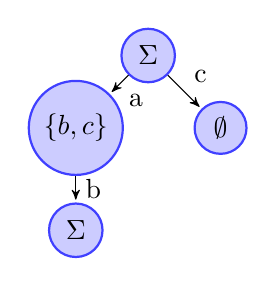
\begin{tikzpicture}[node distance=1.3cm,>=stealth',bend angle=45,auto]
  \tikzstyle{place}=[circle,thick,draw=blue!75,fill=blue!20,minimum size=6mm]
  \tikzstyle{red place}=[place,draw=red!75,fill=red!20]
  \tikzstyle{transition}=[rectangle,thick,draw=black!75,
  			  fill=black!20,minimum size=4mm]
  \tikzstyle{every label}=[red]
  
  \begin{scope}
    \node [place] (w1) {$\Sigma$};
    \node [place] (e1) [below left of=w1] {$\{b,c\}$}
      edge [pre]  node[swap] {a}                 (w1);      
    \node [place] (e2) [below right of=w1] {$\emptyset$}
      edge [pre]  node[swap] {c}                 (w1);      
    \node [place] (e3) [below of=e1] {$\Sigma$}
      edge [pre]  node[swap] {b}                 (e1);      
  \end{scope}
    
\end{tikzpicture}
\caption{Example model.}\label{figure:elSmall}
\end{FIGURE}



We continue with concrete examples.  The model in Figure
\ref{figure:elSmall} satisfies all the following formulae, amongst
others:
\[
\begin{array}{lclclclcl}
\MAY{a} &\qquad&
\MAY{a} \MAY{b} &\qquad&
\MAY{a} \fBang \{b,c\} &\qquad&
\MAY{a} \fBang \{b,c,d\} &\qquad&
\MAY{c} \\[1mm]
\MAY{c} \fBang \{\} &&
\MAY{c} \fBang \{a\} &&
\MAY{c} \fBang \{a,b\} &&
\MAY{a} \land \MAY{c} &&
\MAY{a} (\MAY{b} \land \fBang \{b,c\}
\end{array}
\]

\NI Here we assume, as we do with all subsequent such figures, that
the top note is the root.  The same model does \emph{not} satisfy any
of the following formulae
\[
\MAY{b} \qquad
\fBang \{a\} \qquad
\fBang \{a, c\} \qquad
\MAY{a} \fBang \{b\} \qquad
\MAY{a} \MAY{c} \qquad
\MAY{a} \MAY{b} \fBang \{c\} 
\]

\NI Figure \ref{threemodels} shows various models of $\MAY{a} \MAY{b}$
and Figure \ref{more models} shows one model that does, and one that
does not, satisfy the formula $\fBang \{a,b\}$.  Both models validate
$!\{a, b, c\}$.

\Cathoristic{} does not have the operators $\neg, \lor, $ or $\Rightarrow$.
This has the following two signification consequences.  First, every
satisfiable formula has a unique (up to isomorphism) simplest model.
In Figure \ref{threemodels}, the left model is the unique simplest
model satisfying$\MAY{a} \MAY{b}$.  We will clarify below that model
simplicity is closely related to the process theoretic concept of
similarity, and use the existence of unique simplest models to
construct a \emph{quadratic-time} decision procedure.

\begin{FIGURE}
\centering
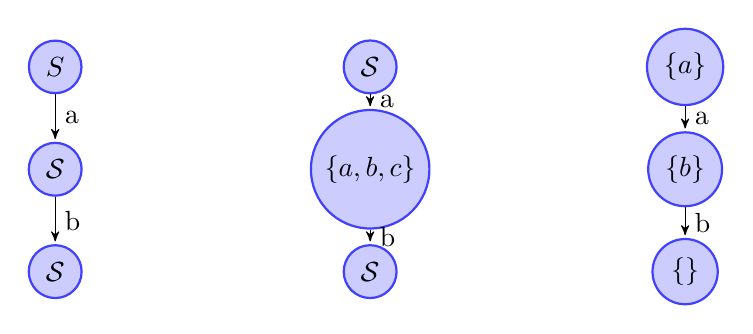
\begin{tikzpicture}[node distance=1.3cm,>=stealth',bend angle=45,auto]
  \tikzstyle{place}=[circle,thick,draw=blue!75,fill=blue!20,minimum size=6mm]
  \tikzstyle{red place}=[place,draw=red!75,fill=red!20]
  \tikzstyle{transition}=[rectangle,thick,draw=black!75,
  			  fill=black!20,minimum size=4mm]
  \tikzstyle{every label}=[red]
  \begin{scope}[xshift=0cm]
    \node [place] (w1) {$S$};
    \node [place] (e1) [below of=w1] {$\mathcal{S}$}
      edge [pre]  node[swap] {a}                 (w1);
    \node [place] (e2) [below of=e1] {$\mathcal{S}$}
      edge [pre]  node[swap] {b}                 (e1);
  \end{scope}   
  \begin{scope}[xshift=4cm]
    \node [place] (w1) {$\mathcal{S}$};
    \node [place] (e1) [below of=w1] {$\{a,b,c\}$}
      edge [pre]  node[swap] {a}                 (w1);
    \node [place] (e2) [below of=e1] {$\mathcal{S}$}
      edge [pre]  node[swap] {b}                 (e1);
  \end{scope}   
  \begin{scope}[xshift=8cm]
    \node [place] (w1) {$\{a\}$};
    \node [place] (e1) [below of=w1] {$\{b\}$}
      edge [pre]  node[swap] {a}                 (w1);
    \node [place] (e2) [below of=e1] {$\{\}$}
      edge [pre]  node[swap] {b}                 (e1);
  \end{scope}   
\end{tikzpicture}
\caption{Various models of $\langle a \rangle \langle b \rangle \top$}
\end{FIGURE}


\begin{FIGURE}
\centering
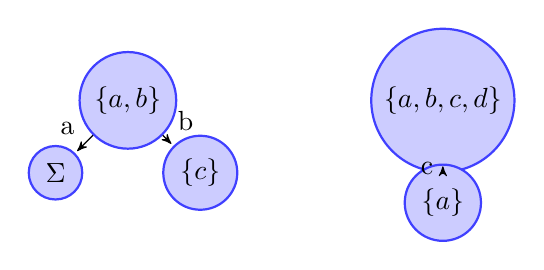
\begin{tikzpicture}[node distance=1.3cm,>=stealth',bend angle=45,auto]
  \tikzstyle{place}=[circle,thick,draw=blue!75,fill=blue!20,minimum size=6mm]
  \tikzstyle{red place}=[place,draw=red!75,fill=red!20]
  \tikzstyle{transition}=[rectangle,thick,draw=black!75,
  			  fill=black!20,minimum size=4mm]
  \tikzstyle{every label}=[red]
  \begin{scope}[xshift=0cm]
    \node [place] (w1) {$\{a, b\}$};
    \node [place] (e1) [below left of=w1] {$\Sigma$}
      edge [pre]  node {a}                 (w1);
    \node [place] (e2) [below right of=w1] {$\{c\}$}
      edge [pre]  node[swap] {b}                 (w1);
  \end{scope}   
  \begin{scope}[xshift=4cm]
    \node [place] (w1) {$\{a, b, c, d\}$};
    \node [place] (e1) [below of=w1] {$\{a\}$}
      edge [pre]  node[swap] {c}                 (w1);
  \end{scope}   
\end{tikzpicture}
\caption{The model on the left validates $!\{a, b, c\}$
while the model on the right does not.}\label{figure:elAndBang:moreMdels}
\end{FIGURE}


Secondly, EL is different from other logics in that there is an
asymmetry between tautologies and contradictories: logics with
conventional negation have an infinite number of non-trivial
tautologies as well as an infinite number of contradictories.  In
contrast, because \cathoristic{} has no negation or disjunction
operator, it is expressively limited in the tautologies it can
express: top and conjunctions of top are its sole tautologies. On the
other hand, the tantum operator, enables an infinite number of
contradictories to be expressed.  For example:
\[
   \MAY{a} \land \fBang \{\} \qquad
   \MAY{a} \land \fBang \{b\} \qquad
   \MAY{a} \land \fBang \{b, c\} \qquad
   \MAY{b} \land \fBang \{\} \qquad
\]


%% \begin{definition} Let $\Gamma$ be an arbitrary set of formulae. We
%% say \emph{$\Gamma$ semantically implies $\phi$}, written $\Gamma
%% \models \phi$, provided for all cathoristic models $\MMM$ if it is the
%% case that $\MMM \models \Gamma$ implies $\MMM \models \phi$.
%% \richard{We do not define $\models \Gamma$ for a set $\Gamma$, only
%% for individual formulae - do we want to change this definition to
%% be of the form $\phi \models \psi$?}  \end{definition}

\NI The semantic consequence relation is standard.\martin{actually
  it's not because the premise can have only one formula. Maybe we
  should elaborate upon this? I think it's intimately related to the
  absence of negation. In classical logic we can use $\Gamma \models
  \phi$ because only a finite bit already implies $ \phi$ and that can
  easily be proven. In EL ... not so much}

\begin{definition} 
 We say the formula $\phi$ \emph{semantically implies} $\psi$, written $\phi
   \models \psi$, provided for all cathoristic models $\MMM$ if it is the
   case that $\MMM \models \phi$ then also $\MMM \models \phi$.
\end{definition}

\begin{example}
\Cathoristic{} shares with other (multi)-modal logics the following
implications:
\begin{eqnarray*}
\MAY{a} \MAY{b} \models \MAY{a} 
 \qquad\qquad
\MAY{a} (\MAY{b} \land \MAY{c}) \models \MAY{a} \MAY{b}
\end{eqnarray*}
As \cathoristic{} is restricted to deterministic models, it also
validates the following formula:
\begin{eqnarray*}
\MAY{a} \MAY{b} \land \MAY{a} \MAY{b}  \models \MAY{a} (\MAY{b} \land \MAY{c})
\end{eqnarray*}
\Cathoristic{} also validates all implications in which the set of constraints is relaxed from left to right. For example:
\begin{eqnarray*}
\fBang \{\} \models \fBang \{a\} 
 \qquad\qquad
\fBang \{\} \models \fBang \{a, b\} 
\end{eqnarray*}
\end{example}


\section{Capturing Inferences Between Atomic Sentences}\label{naturalLanguageInference}

\NI \Cathoristic{} arose as an attempt to answer the question: what is the
simplest logic that can capture inferences between atomic sentences of
natural language?  In this section, we enumerate the sorts of
inferences we are trying to capture.  Then we show how \cathoristic{}
handles these inferences.  Finally, we compare our approach with the
various attempts at expressing the inferences in first-order logic.

\subsection{Intra-Atomic Inferences in Natural Language}

\NI Natural language admits many types of inference between atomic
sentences.  First, exclusion:
\begin{quote}
``Jack is male'' is incompatible with ``Jack is female''
\end{quote}
Second, entailment inferences from dyadic to monadic predicates:
\begin{quote}
``Jack loves Jill'' implies ``Jack loves''
\end{quote}
Third, adverbial inferences:
\begin{quote}
``Jack walks quickly'' implies ``Jack walks''
\end{quote}
Fourth, inferences from conjunctions of sentences to conjunctions of noun-phrases (and vice-versa):
\begin{quote}
``Jack loves Jill'' and ``Jack loves Joan'' together imply that ``Jack loves Jill and Joan''
\end{quote}
Fifth, inferences from conjunctions of sentences to conjunction of predicates\footnote{See \cite{sommers} p.282 for a spirited defence of predicate conjunction against Fregean regimentation.} (and vice-versa):
\begin{quote}
``Jack is bruised'' and ``Jack is humiliated'' together imply that ``Jack is bruised and humiliated''.
\end{quote}

\NI They all can be handled directly and naturally in \cathoristic{}, as we
shall now show.


\subsection{Intra-Atomic Inferences in \Cathoristic{}}
%% We shall show that each of the following inferences can be naturally expressed in \cathoristic{}:
%% \begin{itemize}
%% \item
%% ``Jack is male'' is incompatible with ``Jack is female''
%% \item
%% ``Jack loves Jill'' implies ``Jack loves''\footnote{Although natural languages are full of examples of inferences from dyadic to monadic predicates, there are certain supposed counterexamples to the general rule that a dyadic predicate always implies a monadic one. For example, ``Jack explodes the device'' does not, on its most natural reading, imply that ``Jack explodes''. Our response to cases like this is to distinguish between two distinct monadic predicates $explodes_1$ and $explodes_2$:
%% \begin{itemize}
%% \item
%% $X explodes_1$ iff $X$ is an object that undergoes an explosion
%% \item
%% $X explodes_2$ iff $X$ is an agent that initiates an explosion
%% \end{itemize}
%% Now ``Jack explodes the device'' does imply that ``Jack $explodes_2$'' but does not imply that ``Jack $explodes_1$''. 
%% There is no deep problem here - just another case where natural language overloads the same word in different situation to have different meanings.}
%% \item
%% ``Jack walks quickly'' implies ``Jack walks''
%% \item
%% ``Jack loves Jill'' and ``Jack loves Joan'' together imply that ``Jack loves Jill and Joan''
%% \item
%% ``Jack is bruised'' and ``Jack is humiliated'' together imply that ``Jack is bruised and humiliated''.
%% \end{itemize}

Incompatibility such as that between ``Jack is male'' and ``Jack is
female'' is translated into \cathoristic{} as the pair of incompatible
sentences:
\begin{eqnarray*}
\MAY{jack} \MAY{sex} (\MAY{male} \land \fBang \{male\}) 
   \qquad\qquad
\MAY{jack} \MAY{sex} (\MAY{female} \land \fBang \{female\})
\end{eqnarray*}

\NI Entailment from dyadic to monadic predicates\footnote{Although natural languages are full of examples of inferences from dyadic to monadic predicates, there are certain supposed counterexamples to the general rule that a dyadic predicate always implies a monadic one. For example, ``Jack explodes the device'' does not, on its most natural reading, imply that ``Jack explodes''. Our response to cases like this is to distinguish between two distinct monadic predicates $explodes_1$ and $explodes_2$:
 \begin{itemize}
 \item
 $X explodes_1$ iff $X$ is an object that undergoes an explosion
 \item
 $X explodes_2$ iff $X$ is an agent that initiates an explosion
 \end{itemize}
 Now ``Jack explodes the device'' does imply that ``Jack $explodes_2$'' but does not imply that ``Jack $explodes_1$''. 
There is no deep problem here - just another case where natural language overloads the same word in different situation to have different meanings.}:
``Jack loves Jill'' is translated into \cathoristic{} as:
\begin{eqnarray*}
   \MAY{jack} \MAY{loves} \MAY{jill}
\end{eqnarray*}
The semantics of modalities ensures that this directly entails:
\begin{eqnarray*}
   \MAY{jack} \MAY{loves}
\end{eqnarray*}

\NI Similarly, \cathoristic{} supports inferences from triadic to dyadic
predicates:
\begin{quote}
  ``Jack passed the biscuit to Mary'' implies ``Jack passed the biscuit''
\end{quote}

\NI This can be expressed directly in \cathoristic{} as:
\[
   \MAY{jack} \MAY{passed} \MAY{biscuit} \MAY{to} (\MAY{mary} \land !\{mary\}) \models \MAY{jack} \MAY{passed} \MAY{biscuit}
\]

\NI Adverbial inferences is captures in \cathoristic{} as follows.
\begin{eqnarray*}
\MAY{jack} \MAY{walks} \MAY{quickly}
\end{eqnarray*}
entails:
\begin{eqnarray*}
\MAY{jack} \MAY{walks}
\end{eqnarray*}

\NI \Cathoristic{} directly supports inferences from conjunctions of
sentences to conjunctions of noun-phrases.  As our models are
deterministic, we have the general rule that $ \MAY{a} \MAY{b} \land
\MAY{a} \MAY{c} \models \MAY{a} (\MAY{b} \land \MAY{c})$ from which
it follows that
\begin{eqnarray*}
   \MAY{jack} \MAY{loves} \MAY{jill}
      \qquad\text{and}\qquad
   \MAY{jack} \MAY{loves} \MAY{joan}
\end{eqnarray*}
together imply
\begin{eqnarray*}
\MAY{jack} \MAY{loves} (\MAY{jill} \land \MAY{joan})
\end{eqnarray*}

\NI Using the same rule, we can infer that
\begin{eqnarray*}
   \MAY{jack} \MAY{bruised} \land \MAY{jack} \MAY{humiliated}
\end{eqnarray*}

\NI together imply
\begin{eqnarray*}
\MAY{jack} (\MAY{bruised} \land \MAY{humiliated})
\end{eqnarray*}
 
\subsection{Representing incompatible predicates in \FOL}\label{incompatiblepredicatesinfol}

\NI How are incompatible predicates represented in traditional
\fol{}?  Brachman and Levesque\cite{brachman} introduce the
topic of incompatible predicates by remarking:
\begin{quote}
   We would consider it quite ``obvious'' in this domain that if it
   were asserted that $John$ were a $Man$, then we should answer
   ``no'' to the query $Woman(John)$.
\end{quote}

\NI They propose adding an extra axiom to express the incompatibility:
\[
   \forall x. ( Man(x) \rightarrow \neg Woman(x) )
\]  
 
\NI This proposal imposes an authoring burden on the
knowledge-representer.  We would have to add an extra axiom for every
pair of incompatible predicates.  This proposal becomes particularly
burdensome when dealing with large sets of incompatible predicates.
For example, suppose there are 50 football teams, and a person can
only support one team at a time.  We would need to add $C \cdot {50 \choose 2}$
axioms: incompatibility axioms would become large and unwieldy:
\[
\begin{array}{l}
  \forall x.  \neg (SupportsArsenal(x) \land SupportsLiverpool(x))  \\
  \forall x.  \neg (SupportsArsenal(x) \land SupportsManUtd(x))  \\
  \forall x.  \neg (SupportsLiverpool(x) \land SupportsManUtd(x))  \\
  \qquad \qquad \qquad \vdots
\end{array}
\]

\NI Or, if we treat the football-teams as objects, and have a
two-place $Supports$ relation between people and teams, we could have:
\[
   \forall x, y, z. (Supports(x,y) \land y \neq z \rightarrow \neg Supports(x,z))
\]   

\NI Together with the Unique Names Assumption (which lets us assume
that each football team is distinct from all the others), this
certainly captures the desired uniqueness condition.  But it does so
by using relatively complex logical machinery.

\subsection{Supporting Inferences from Dyadic to Monadic Predicates in Predicate Logic}
If we want to capture the inference from ``Jack loves Jill`` to ``Jack loves'' in \fol{}, we have to add a non-logical axiom:
\[
(\forall x, y) Loves(x,y) \rightarrow Loves(x)
\]

\NI We would have to add an extra non-logical axiom like this for every
n-place predicate.  This is cumbersome at best.  In \cathoristic{}, by
contrast, we do not need to introduce any non-logical machinery at all
to capture these inferences because they all follow from the general
rule that $\MAY{a} \MAY{b} \models \MAY{a}$.

\subsection{Supporting adverbial inferences in \fol{}}

\NI How can we represent verbs in traditional \fol{} so as to
support adverbial inference?  Davidson \cite{davidson2} proposed that
every $n$-place action verb be analysed as an $n$+1-place predicate,
with an additional slot representing an event.  For example, he
analysed ``I flew my spaceship to the Morning Star'' as
\[
\exists x. ( Flew(I, MySpaceship, x) \land To(x, TheMorningStar))
\]
This implies 
\[
\exists x.  Flew(I, MySpaceship, x)
\]
This captures the inference from ``I flew my spaceship to the Morning Star'' to ``I flew my spaceship''.

Predicate Logic cannot support logical inferences between elementary propositions. 
If it is going to support inferences from adverbial sentences, it \emph{cannot} treat them as elementary propositions and must instead \emph{reinterpret} them as logically complex propositions.
The cost of Davidson's proposal is that a seemingly simple sentence, such as ``Jones walks'', turns out on closer inspection not be elementary at all,  but to involve existential quantification:
\[
\exists x.  Walks(Jones, x)
\]

\NI Although Predicate Logic can handle some of these inferences, it
can only do so by reinterpreting the sentences as logically-complex
compound propositions.

\subsection{Summary}
We have looked at various types of inference between atomic
sentences. \Cathoristic{} can handle them directly and naturally.  Traditional
\fol{} has a harder time: it
\emph{can} express incompatibility, but only using complex machinery -
universal quantification, a conditional, negation. \Cathoristic{}, by
contrast, expresses the source of the incompatibility \emph{directly}
using the $!$ operator.  Again, \fol{} \emph{can} express
adverbial inferences, but at the cost of using quantification over
events.  When it comes to inferences from conjunctions of sentences to
conjunctions of noun-phrases (or predicates), \fol{} has
nothing to say because it has no way of expressing conjunctions
between noun-phrases (or predicates) \emph{at all}. In \fol{}, ``Jack is bruised and humiliated'' has to be regimented into
``Jack is bruised and Jack is humiliated''.  This might seem, to the uninitiated, to be the
wrong way around.  

However, \cathoristic{} cannot handle all instances
of sub-propositional inferences.  An example are inferences where the
\emph{subjects} are conjoined such as
\begin{quote}
``Jack loves Jill'' and ``Jim loves Jill'' together imply that ``Jack and Jim love Jill''
\end{quote}

\NI \Cathoristic{} has no way to conjoin noun-phrases in subject-position.

\section{\Cathoristic{} as a language for knowledge representation}\label{kr}


\Cathoristic{} has been used as the representation language for a
large, complex, dynamic multi-agent simulation \cite{evans-and-short}.
This is an industrial-sized application, involving tens of thousands
of rules and facts\footnote{The application has thousands of paying
  users, and available for download on the App Store for the iPad
  \cite{Versu}.}.  In this simulation, the entire world state is stored
as a set of \cathoristic{} formulae - all other aspects of world state
are transient and computed as needed.  The current true sentences are
represented in a cathoristic model.\martin{THis is inconsistent: are the facts stored as CL formulae or a CL model?}

We shall first sketch how facts are represented, before describing some
advantages of \cathoristic{} over a more traditional \fol{}
representation of knowledge.

\subsection{Representing facts  in \cathoristic{}}

A sentence involving a one-place predicate of the form $p(a)$ is
expressed in \cathoristic{} as
\begin{eqnarray*}
   \MAY{a} \MAY{p}.
\end{eqnarray*}

\NI A sentence involving a many-to-many two-place relation of the form
$r(a,b)$ is expressed in \cathoristic{} as
\begin{eqnarray*}
  \MAY{a} \MAY{r} \MAY{b}.
\end{eqnarray*}

\NI But a sentence involving a many-to-one two-place relation of the
form $r(a,b)$ is expressed as:
\begin{eqnarray*}
  \MAY{a} \MAY{r} (\MAY{b} \land \fBang \{b\}).
\end{eqnarray*}

\NI The translation is detailed in Section \ref{translationFOLtoFOEL}.

So, for example, to say that ``Jack likes Jill'' (where ``likes'' is,
of course, a many-many relation), we would write:
\begin{eqnarray*}
  \MAY{jack} \MAY{likes} \MAY{jill}.
\end{eqnarray*}

\NI But to say that ``Jack is married to Joan''
(where``is-married-to'' is a many-one relation), we would write:
\begin{eqnarray*}
  \MAY{jack} \MAY{married} (\MAY{joan} \land \fBang \{joan\}).
\end{eqnarray*}

\NI Colloquially, we might say that ``Jack is married to Joan - and
only Joan''.  Note that the relations are placed in infix position, so
that the facts about an object are ``contained'' within the object.
One reason for this particular way of structuring the data will be
explained below.
 
\martin{ I think the rest of this section could be structured more
  clearly. I think we are saying CL is good for the following two
  (very different) reasons.  (1) Convenience of representation for
  humans. (2) Algorithmic properties, which are about (a) efficient
  model update and (b) efficient queries. CL is good regarding (2)
  because formulae have tree structure and trees can be efficiently
  represented using pointers manipulated using lot's of well-known
  algorithms. Maybe state the general picture first and then give
  examples?}

Consider the following facts about a gentleman named Brown:

\[
   \MAY{brown} 
   \left(
   \begin{array}{l}
     \MAY{sex} (\MAY{male} \land \fBang \{male\}) \\
        \qquad \AND \\
     \MAY{friends} (\MAY{lucy} \land \MAY{elizabeth}) 
   \end{array}
   \right)
\]

\NI All facts  starting with the prefix $\MAY{brown}$ form a
sub-tree of the entire database.  And all  facts which start with
the prefix $\MAY{brown} \MAY{friends}$ form a sub-tree of that tree.
A sub-tree can be treated as an individual via its prefix.  
A sub-tree of formulae is the \cathoristic{} equivalent of an
\emph{object} in an object-oriented programming language.

To model change over time, we assert and retract statements from the
database, using a non-monotonic update mechanism.  If a fact is
inserted into the database that involves a state-labelling restricting
the permissible  transitions emanating from that state, then all
transitions out of that state that are incompatible with the
restriction are removed.  So, for example, if the database currently
contains the fact that the traffic light is amber, and then we update
the database to assert the traffic light is red:
\[
\MAY{tl} \MAY{colour} (\MAY{red} \land !\{red\})
\]
Now the restriction on the state (that red is the only transition)
means that the previous transition from that state (the transition
labelled with amber) is automatically removed.

The tree-structure of formulae allows us to express the \emph{life-time of data} in a natural way. 
If we wish a piece of data $d$ to exist for just the duration of a proposition $t$, then we make $t$ be a sub-expression of $d$. 
For example, if we want the friendships of an agent to exist just as long as the agent, then we place the relationships inside the agent: 
\[
\MAY{brown} \MAY{friends}
\]
Now, when we remove $\MAY{brown}$ all the sub-trees, including the data about who he is friends with, will be automatically deleted as well.

Another advantage of our representation is that we get a form of \emph{automatic currying} which simplifies queries.
So if, for example, Brown is married to Elizabeth, then the database would contain 
\begin{eqnarray*}
\MAY{brown} \MAY{married} (\MAY{elizabeth} \land \fBang \{elizabeth\})
\end{eqnarray*}
In \cathoristic{}, if we want to find out whether Brown is married, we can query the sub-formula directly -  we just ask if 
\begin{eqnarray*}
\MAY{brown} \MAY{married}
\end{eqnarray*}
In \fol, if $married$ is a two-place predicate, then we need to fill in the extra argument place with a free variable - we would need to find out if there exists an $X$ such that $married(brown, X)$ - this is slower to compute and more cumbersome to type. 

\subsection{Simpler postconditions}

In this section, we contrast the representation in action languages based on \fol{}\footnote{E.g. STRIPS \cite{strips}}, with our \cathoristic{}-based representation.
Action definitions are rendered in typewriter font.

When expressing the pre- and post-conditions of an action, planners
based on \fol{} have to explicitly describe the propositions that
are removed when an action is performed:
\begin{verbatim}
   action move(A, X, Y)
       preconditions
           at(A, X)
       postconditions
           add: at(A, Y) 
           remove: at(A, X)
\end{verbatim}
Here, we need to explicitly state that when $A$ moves from $X$ to $Y$, $A$ is no longer at $X$. It might seem obvious to us that if $A$ is now at $Y$, he is no longer at $X$ - but we need to explicitly tell the system this. This is unnecessary, cumbersome and error-prone. In \cathoristic{}, by contrast, the exclusion operator means we do not need to specify the facts that are no longer true:
\begin{verbatim}
   action move (A, X, Y)
       preconditions
           <A><at>(<X> /\ !{X})
       postconditions
           add: <A><at>(<Y> /\ !{Y})
\end{verbatim}
The tantum operator $!$ makes it clear that something can only be at one
place at a time, and the non-monotonic update rule described above
\emph{automatically} removes the old invalid location data.

\subsection{Using tantum $!$  to optimise preconditions}
\label{optimizingpreconditions}
Suppose, for example, we want to find all married couples who are both Welsh.
In Prolog, we might write something like:
\begin{verbatim}
   welsh_married_couple(X, Y) :-
       welsh(X),
       welsh(Y),
       spouse(X,Y).
\end{verbatim}	
Rules like this create a large search-space because we need to find all instances of $welsh(X)$ and all instances of  $welsh(Y)$ and take the cross-product \cite{smith-and-genesereth}. If there are $n$ Welsh people, then we will be searching $n^2$ instances of $(X,Y)$ substitutions.

If we express the rule in \cathoristic{}, the compiler is able to use the extra information expressed in the $!$ operator to reorder the literals to find the result significantly faster.
Assuming someone can only have a single spouse at any moment, the rule is expressed in \cathoristic{} as:
\begin{verbatim}
   welsh_married_couple(X, Y) :-
       <welsh> <X>,
       <welsh> <Y>,
       <spouse> <X> (<Y> /\ !{Y}).
\end{verbatim}	
Now the compiler is able to reorder these literals to minimize the search-space. 
It can see that, once $X$ is instantiated, the following literal can be instantiated without increasing the search-space:
\begin{verbatim}
   <spouse> <X> (<Y> /\ !{Y})
\end{verbatim}
The \emph{tantum} operator can be used by the compiler to see that there is at most one $Y$ who is the spouse of $X$.
So the compiler reorders the clauses to produce:
\begin{verbatim}
   welsh_married_couple (X, Y) :-
       <welsh> <X>,
       <spouse> <X> (<Y> /\ !{Y}),
       <welsh> <Y>.
\end{verbatim}	
Now it is able to find all results by just searching $n$ instances - a significant optimization.
In our application, this optimisation has made a significant difference to the run-time cost of query evaluation.







\section{\ELFULL}\label{coreEL}

In this section we introduce the syntax and semantics of \ELFULL{}
(hereafter \ELABR{}).  Then we establish key completeness of the the
proof rules and prove a the compactness theorem via a translation into
first-order logic. We focus on a small core of \ELABR{}, leaving
extensions to later section.

\subsection{Syntax}

\NI Syntactically, eremic logic is a multi-modal logic with one new
operator.

\begin{definition} Let $\Sigma$ be a non-empty set of \emph{actions}.
Actions are ranged over by $a, a', a_1, b, ...$, and $A$ ranges over
finite subsets of $\Sigma$. The \emph{formulae}, ranged over by $\phi,
\psi, \xi ...$, of \ELABR{} are given by the
following grammar.

\begin{GRAMMAR}
  \phi 
     &\quad ::= \quad & 
  \TRUE 
     \VERTICAL 
  \phi \AND \psi
     \VERTICAL 
  \MAY{a}{\phi}
     \VERTICAL 
  \fBang A 
\end{GRAMMAR}
\end{definition}

\NI  Before presenting models and the satisfaction relation, we sketch
the meaning of formulae informally. $\TRUE$ is truth and $\phi \AND
\psi$ is the conjunction of formulae $\phi$ and $\psi$. Clearly
$\MAY{a}{\phi}$ is the may-modality which asserts that the current
state may do action $a$ and in doing $a$ transitions into a now state
at which $\phi$ holds.  The key novelty of eremic logic is $!A$,
pronounced ``just $A$, or ``tantum $A$. The core intuition about $!A$
is that if a model validates $!A$ at the current state, then the only
modalities $\MAY{a}{}$ available at the corrent state are those with
$a \in A$. 

The set of actions must be non-empty to avoid that the logic is
trivial. The restriction to finite subsets of action substantially
simplifies the meta-theory of the logic.

We often abbreviate $\MAY{a}{\TRUE}$ to $\MAY{a}{}$. We define falsity
$\FALSE$ as $!\emptyset \AND \MAY{a}{}$ where $a$ is an arbitrary
action. Note that in the absence of conventional negation, we cannot
readily define disjunction, implication, or must-modalities by de
Morgan duality. We discuss later \martin{Where?} how some of the usual
propositional connectives can be (partially) recovered. \martin{What
  about must modalities?}

\begin{convention}
From now on we assume a fixed set $\Sigma$ of actions, except where
stated otherwise.
\end{convention}

\subsection{Semantics}

\NI The semantics of eremic logic is close to Hennessy-Milner logic
\cite{HennessyM:alglawfndac} and uses labelled transition systems, as
described in Section \ref{preliminaries}, but augmented with labels on
states.

\begin{definition}
An \emph{eremic transition system} is a triple $(S, \rightarrow,
\lambda)$, where $(S, \rightarrow)$ is a labelled transition system
over $\Sigma$, and $\lambda$ is a function from states to sets of
actions (not necessarily finite), subject to the following constraints:
\begin{itemize}

\item For all states $s \in S$ it is the case that $ \{a \fOr \exists
  t \; s \xrightarrow{a} t\} \subseteq \lambda(s)$. We call this
  condition \emph{admissibility}.

\item For all states $s \in S$, $\lambda (s)$ is either finite or
  $\Sigma$. We call this condition \emph{well-sizedness}.

\end{itemize}

\end{definition}

\NI The intended interpretation is that $\lambda(w)$ is the set of
allowed transition symbols emanating from $w$.  The $\lambda$ function
is the semantic counterpart of the $!$ operator.  The admissibility
restriction is in place because transitions $s \TRANS{a} t$ where $a
\notin \lambda(s)$ would be saying that an $a$ action is possible at
$s$ but at the same time prohibit $a$ actions at that state.
Well-sizedness is not a fundamental restriction but rather a
convenient trick. Essentially eremic transition systems have two kinds
of nodes:

\begin{itemize}

\item Nodes $s$ without restrictions on outgoing transitions. Those are
  labelled with $\lambda ( s) = \Sigma$.

\item Nodes $s$ with restriction on outgoing transitions. Those are
  labelled by a finite set $\lambda ( s)$ of actions.

\end{itemize}

\NI Defining $\lambda$ on all nodes and not just on those with
restrictions makes some definitions and proofs slightly easier.

As with outher modal logics, satisfaction of formulae is defined
relative to a state in the ambient eremic transition system, giving
rise to the following definition.

\begin{definition}
A \emph{eremic model}, ranged over by $\MMM, \MMM', ...$, is a pair $(\LLL,
s)$, where $\LLL$ is an eremic transition system $(S, \rightarrow,
\lambda)$, and $s$ is a state from $S$.
\end{definition}

\NI With eremic models at hand, we can finally formalise the
satisfaction relation for eremic formulae.

\begin{definition}
The \emph{satisfaction relation} $\MMM \models \phi$ is defined
inductively by the following clauses, where we assume that $\MMM =
(\LLL, s)$ and $\LLL = (S, \rightarrow, \lambda)$.

\[
\begin{array}{lclcl}
  \MMM & \models & \top   \\
  \MMM & \models & \phi \AND \psi &\ \mbox{ iff } \ & \MMM  \models \phi \mbox { and } \MMM \models \psi  \\
  \MMM & \models & \langle a \rangle \phi & \mbox{ iff } & \text{there is a } s \xrightarrow{a} t \mbox { such that } (\LLL, t) \models \phi  \\
  \MMM & \models & \fBang A &\mbox{ iff } & \lambda(s) \subseteq A
\end{array}
\]

\end{definition}

\NI The first three clauses are standard, and Figure
\ref{figure:elAndBang:models} gives examples of models for the formula
$\MAY{a}{\MAY{b}{\TRUE}}$.  The last clause enforces the intended
meaning of $!A$: the available modalities in the model are \emph{at
  least as constrainted} as required by $!A$. They may even be more
constrainted, if the inclusion $\lambda(s) \subseteq A$ is proper. We
note in the case where the set $\Sigma$ of actions is infinite,
allowing $\lambda(s)$ to return arbitrary inifinite sets in addition
to $\sigma$ does not make a difference because $A$ is finite by
construction, so $\lambda(s) \subseteq A$ can never hold when
$\lambda(s)$ is infinite. Figure \ref{figure:elAndBang:moreMdels}
presents examples of validating (and otherwise) the formula $!\{a, b,
c\}$.

\begin{FIGURE}
\centering
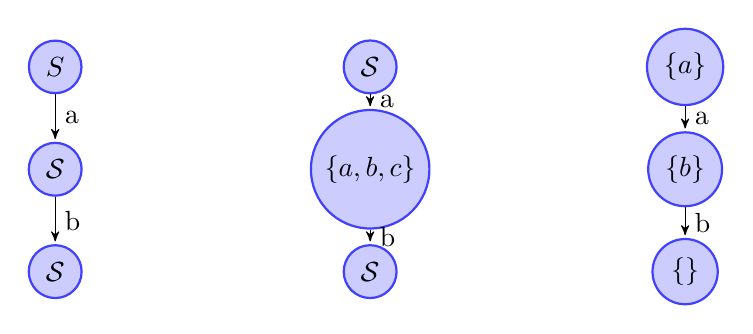
\begin{tikzpicture}[node distance=1.3cm,>=stealth',bend angle=45,auto]
  \tikzstyle{place}=[circle,thick,draw=blue!75,fill=blue!20,minimum size=6mm]
  \tikzstyle{red place}=[place,draw=red!75,fill=red!20]
  \tikzstyle{transition}=[rectangle,thick,draw=black!75,
  			  fill=black!20,minimum size=4mm]
  \tikzstyle{every label}=[red]
  \begin{scope}[xshift=0cm]
    \node [place] (w1) {$S$};
    \node [place] (e1) [below of=w1] {$\mathcal{S}$}
      edge [pre]  node[swap] {a}                 (w1);
    \node [place] (e2) [below of=e1] {$\mathcal{S}$}
      edge [pre]  node[swap] {b}                 (e1);
  \end{scope}   
  \begin{scope}[xshift=4cm]
    \node [place] (w1) {$\mathcal{S}$};
    \node [place] (e1) [below of=w1] {$\{a,b,c\}$}
      edge [pre]  node[swap] {a}                 (w1);
    \node [place] (e2) [below of=e1] {$\mathcal{S}$}
      edge [pre]  node[swap] {b}                 (e1);
  \end{scope}   
  \begin{scope}[xshift=8cm]
    \node [place] (w1) {$\{a\}$};
    \node [place] (e1) [below of=w1] {$\{b\}$}
      edge [pre]  node[swap] {a}                 (w1);
    \node [place] (e2) [below of=e1] {$\{\}$}
      edge [pre]  node[swap] {b}                 (e1);
  \end{scope}   
\end{tikzpicture}
\caption{Various models of $\langle a \rangle \langle b \rangle \top$}
\end{FIGURE}

\begin{FIGURE}
\centering
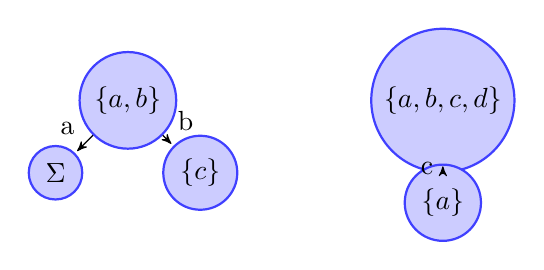
\begin{tikzpicture}[node distance=1.3cm,>=stealth',bend angle=45,auto]
  \tikzstyle{place}=[circle,thick,draw=blue!75,fill=blue!20,minimum size=6mm]
  \tikzstyle{red place}=[place,draw=red!75,fill=red!20]
  \tikzstyle{transition}=[rectangle,thick,draw=black!75,
  			  fill=black!20,minimum size=4mm]
  \tikzstyle{every label}=[red]
  \begin{scope}[xshift=0cm]
    \node [place] (w1) {$\{a, b\}$};
    \node [place] (e1) [below left of=w1] {$\Sigma$}
      edge [pre]  node {a}                 (w1);
    \node [place] (e2) [below right of=w1] {$\{c\}$}
      edge [pre]  node[swap] {b}                 (w1);
  \end{scope}   
  \begin{scope}[xshift=4cm]
    \node [place] (w1) {$\{a, b, c, d\}$};
    \node [place] (e1) [below of=w1] {$\{a\}$}
      edge [pre]  node[swap] {c}                 (w1);
  \end{scope}   
\end{tikzpicture}
\caption{The model on the left validates $!\{a, b, c\}$
while the model on the right does not.}\label{figure:elAndBang:moreMdels}
\end{FIGURE}


\martin{We could Add more examples, maybe ones that we do something with later.}

\begin{definition}
Let $\Gamma$ be an arbitrary set of formulae. We say \emph{$\Gamma$
  semantically implies $\phi$}, written $\Gamma \models \phi$,
provided for all eremic models $\MMM$ if it is the case that $\MMM
\models \Gamma$ implies $\MMM \models \phi$. 
\end{definition}


\subsection{Inference Rules}

\begin{FIGURE}
\begin{RULES}

  \ZEROPREMISERULENAMEDRIGHT
  {
    \phi \judge \phi
  }{Identity}
    \quad
  \ZEROPREMISERULENAMEDRIGHT
  {
    \phi \judge \top
  }{$\top$-Right}
    \quad
  \ZEROPREMISERULENAMEDRIGHT
  {
    \bot \judge \phi
  }{$\bot$-Left}
    \quad
  \TWOPREMISERULENAMEDRIGHT
  {
    \phi \judge \psi
  }
  {
    \psi \judge \xi
  }
  {
    \phi \judge \xi
  }{Transitivity}
    \\\\
  \ONEPREMISERULENAMEDRIGHT
  {
    \phi \judge \psi
  }
  {
    \phi \AND \xi \judge \psi
  }{$\AND$-Left 1}
     \quad
  \ONEPREMISERULENAMEDRIGHT
  {
    \phi \judge \psi
  }
  {
    \xi \AND \phi  \judge \psi
  }{$\AND$-Left 2}
     \quad
  \TWOPREMISERULENAMEDRIGHT
  {
    \phi \judge \psi
  }
  {
    \phi \judge \xi
  }
  {
    \phi \judge \psi \AND \xi
  }{$\AND$-Right}
     \\\\
     \ONEPREMISERULENAMEDRIGHT
     {
       a \notin A
     }
     {
       !A \AND \MAY{a}{\phi} \judge \bot
     }{$\bot$-Right 1}
        \quad
     \ZEROPREMISERULENAMEDRIGHT
     {
       \MAY{a}{\bot} \judge \bot
     }{$\bot$-Right 2}
        \quad
     \TWOPREMISERULENAMEDRIGHT
     {
       \phi \AND \, !A \judge \psi
     }
     {
       A' \subseteq A
     }
     {
       \phi \AND\, !A' \judge \psi
     }{!-Left}
     \\\\
     \TWOPREMISERULENAMEDRIGHT
     {
       \phi \judge !A
     }
     {
       A \subseteq A'
     }
     {
       \phi \judge!A'
     }{!-Right 1}
     \quad
     \TWOPREMISERULENAMEDRIGHT
     {
       \phi \judge !A
     }
     {
       \phi \judge !B
     }
     {
       \phi \judge !(A \cap B)
     }{!-Right 2}
     \quad
     \ONEPREMISERULENAMEDRIGHT
     {
       \phi \judge \psi
     }
     {
       \MAY{a}{\phi} \judge \MAY{a}{\psi}
     }{Transition Normal}
\end{RULES}
\caption{Proof rules.}\label{figure:elAndBangRules}
\end{FIGURE}


\NI We now present the inference rules for \ELFULL{}. There are no
axioms.

\begin{definition} Judgements are of the following form.
\[
  \phi \judge \psi.
\]
Figure \ref{figure:elAndBangRules} presents all proof rules. 
\end{definition}

\NI Note that $\phi$ and $\psi$ are single formulae, not sequents.  By
using single formulae, we can avoid structural inference rules.  \ELABR{}
proof rules can be grouped in two parts: standard rules and rules
unique to \ELABR{}.  Standard rules are [\RULENAME{Identity}],
[\RULENAME{$\top$-Right}], [\RULENAME{$\bot$-Left}],
[\RULENAME{Transitivity}], [\RULENAME{$\AND$-Left 1}],
[\RULENAME{$\AND$-Left 2}] and [\RULENAME{$\AND$-Right}] hardly need
explanation as they are variants of familiar rules for propositional
logic, see e.g.~\cite{TroelstraAS:basprot,vanDalenD:logstr}.  We now
explain the rules that give EL's its distinctive properties: the
relations betwen $\langle \rangle$, $!$ and $\bot$.

The rule [\RULENAME{$\bot$-Right 1}] axiom captures the core
\emph{exclusion} property of !: for example if $A = \{male, female\}$
then $\MAY{orange}{\phi}$ is incompatible with $!A$. Thus $!A \AND
\MAY{orange}{\phi}$ must be false.

The rule [\RULENAME{$\bot$-Right 2}] expresses that falsity is 'global'
  and cannot be surpressed by prefixing. For example
  $\MAY{orange}{\bot}$ is false, simply because $\bot$ is already
  false.

Relatedly, the rule [\RULENAME{Transition Normal}] enables us to
prefix an inference with a may-modality. For example \martin{add good
  example here.}. Note that it is vital for soundness that $\phi$ in $\phi
\judge \psi$ is a single formula. If we used transitional sequents $\phi_1, ..., \phi_n \judge \psi$,
then the rule
\[
   \ONEPREMISERULE
   {
     \phi_1, ..., \phi_n \judge \psi
   }
   {
     \MAY{a}{\phi_1}, ..., \MAY{a}{\phi_n} \judge \MAY{a}{\psi}
   }
\]
is unsound. \martin{explain why, and why this is significant}. This
restriction is also in place in \cite{GaySJ:typcalosp} where a
Curry-Howard corrospondence between a fragment of linear logic
\cite{GirardJY:linlog,GirardJY:protyp} and a process calculus is
introduced. We discuss the relationship between EL and linear logic in
general, and linear logic's additive conjunction in Section
\ref{conclusion}.

Note that the logic has no axioms. One reason for a purely rule-based
presentation is the absence of implication in the present fragment of
EL. \martin{explain in more detail!}

We close this subsection with a key meta-theorem.

\begin{theorem}\label{theorem:elAndBang:soundComplete}
The rules in Figure \ref{figure:elAndBangRules} are sound and complete:
\begin{enumerate}

\item\label{theorem:elAndBang:sound} (Soundness) $\phi \judge \psi$ implies $\phi \models \psi$.

\item\label{theorem:elAndBang:complete} (Completeness) $\phi \models \psi$ implies $\phi \judge \psi$.

\end{enumerate}
\end{theorem}

\NI Soundness is immediate from the definitions. Proof of completeness is
deferred to Section \ref{completenessProof}. 

\begin{definition}
We write $\phi_1, ...,
\phi_n \judge \psi$ whenever $\BIGAND_{i}\phi_i \judge \psi$.  For
arbitrary sets $\Gamma$ of formulae, we write $\Gamma \judge \psi$
provided there are $\phi_1, ..., \phi_n \in \Gamma$ such that $\phi_1,
..., \phi_n \judge \psi$.
\end{definition}

\begin{corollary}\label{theorem:elAndBang:soundComplete}
The rules in Figure \ref{figure:elAndBangRules} are sound and complete:
\begin{enumerate}

\item(Soundness) $\Gamma \judge \psi$ implies $\Gamma \models \psi$.

\item (Completeness) $\Gamma \models \psi$ implies $\Gamma \judge \psi$.\martin{I don't know how to prove it!}

\end{enumerate}
\end{corollary}

\begin{proof}
For soundness assume that $\MMM$ is a model with $\MMM \models
\Gamma$.  We know that $\Gamma \judge \psi$ means that we can find a
finite number of formulae $\phi_i \in \Gamma$ with $\AND_i \phi \judge
\psi$.  By soundness then also $\AND_i \phi \models \psi$, hence
clearly $\Gamma \models \psi$.

For completeness \martin{To do!}
\end{proof}

\subsection{\RULENAME{!-Left} and \RULENAME{!-Right}}

The rules [\RULENAME{!-Right 1}, \RULENAME{!-Right 2}] jointly express
how the subset relation $\subseteq$ on sets of symbols relates to
provability. We don't need a corresponding rule \RULENAME{!-Left}?
for strengthening $!$ on the left hand side
\[
   \TWOPREMISERULENAMEDRIGHT
     {
       \phi \AND \, !A \judge \psi
     }
     {
       A' \subseteq A
     }
     {
       \phi \AND\, !A' \judge \psi
     }{!-Left}
\]
because the latter can be derived from the former:        
\begin{center}
  \AxiomC{$\phi \AND\, !A'  \judge  \phi \AND\, !A'$}
  \AxiomC{$A' \subseteq A$}
  \LeftLabel{\RULENAME{!-Right 1}}
  \BinaryInfC{$\phi \AND\, !A'  \judge  \phi \AND\, !A$}
  \AxiomC{$\phi \AND\, !A  \judge  \psi$}
  \LeftLabel{Transitivity: \quad}
  \BinaryInfC{$\phi \AND\, !A'  \judge  \psi$}
  \DisplayProof
\end{center}
\martin{inconsisten formating of rule names.}

\NI Readers familiar with object-oriented programming will recognise
[\RULENAME{!-Left}] as contra-variant subtyping and [\RULENAME{!-Right
    1}] as covariant subtyping. Honda \cite{HondaK:thetypftpc}
develops a full theory of subtyping based on similar ideas.  All three
rules embody the intuition that whenever $A \subseteq A'$ then
asserting that $!A'$ is as strong as, or a stronger statement than
$!A$. [\RULENAME{!-Left}] simply states that we can always strengthen
our premise, while [\RULENAME{!-right 1}] allows us to weaken the
premise.

\subsection{Example inferences}

We give some example inferences that illustrate how EL is used in
practice.  \martin{Add some example assertions here, for example some
  of those we use later.}
  
\subsection{Proof of completeness}\label{completenessProof}

\NI We now prove completeness of the rules in Figure
\ref{figure:elAndBangRules}.  The proof requires the development of
the following additional technology which is also useful in other
contexts.

\begin{itemize}

\item An ordering $\MODELLEQ$ on models, which enables us to speak of
  the simplest model satisfying a formula.

\item An algorithm which gives the simplest model for a formula.

\item An algorithm which gives the a formula characterising a model.

\end{itemize}

\NI We now develop these three in turn and then prove completeness.

\subsubsection{A partial ordering on models}

We shall define a partial-ordering $\MODELLEQ$ on models by extending
the notion of simulation on labeled transition systems. We then give
an alternative characterisation of $\MODELLEQ$ in terms of
set-inclusion of the theories induced by models.

\begin{definition}
Let $\LLL_i = (S_i, \rightarrow_i, \lambda_i)$ be eremic transition
systems for $i = 1, 2$.  A relation $\RRR \subseteq S_1 \times S_2$ is
a \emph{simulation from $\LLL_1$ to $\LLL_2$}, provided:
\begin{itemize} 

\item $\RRR$ is a simulation on the underlying transition systems. 

\item Whenever $(s, t) \in \RRR$ then also $\lambda_1(s) \supseteq
  \lambda_2(t)$.

\end{itemize}

\NI If $\MMM_i = (\LLL_i, s_i)$ are models, we say $\RRR$ is a
\emph{simulation from $\MMM_1$ to $\MMM_2$}, provided the following hold.

\begin{itemize}

\item $\RRR$ is a simulation from $\LLL_1$ to $\LLL_2$ as eremic transition systems.

\item  $(s_1, s_2) \in \RRR$. 

\end{itemize}
\end{definition}

\begin{definition}
The largest simulation from $\MMM_1$ to $\MMM_2$ is denoted $\MMM_1
\SIM \MMM_2$.  It is easy to see that $\SIM$ is itself a
simulation from $\MMM_1$ to $\MMM_2$, and the union of all such
simulations.  If $\MMM_1 \SIM \MMM_2$ we say $\MMM_2$
\emph{simulates} $\MMM_1$.
\end{definition}

\begin{definition}
Let $\THEORY{\MMM}$ be the \emph{theory} of $\MMM$, i.e.~the formulae
made true by $\MMM$, i.e.~$\THEORY{\MMM} = \{\phi\ |\ \MMM \models
\phi \}$.
\end{definition}

\NI We give an alternative characterisation on $\MODELLEQ$ in terms of
theories of models. In what f`ollows, we will mostly be interested in
$\SIM^{-1}$, so we give it its own symbol.

\begin{definition}
Let $\MODELLEQ$  be short for $\SIM^{-1}$.
\end{definition}

\begin{FIGURE}
\centering
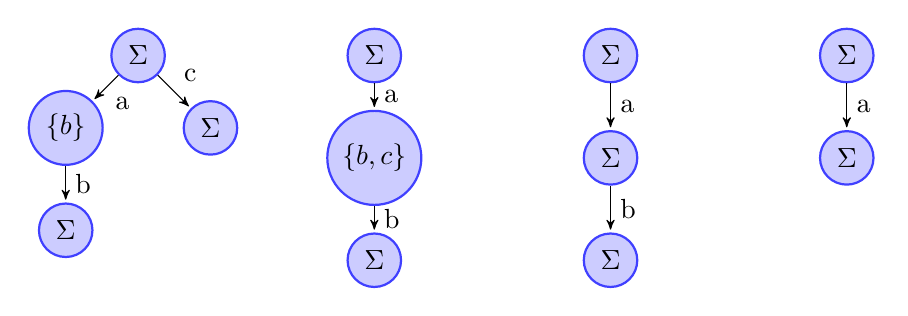
\begin{tikzpicture}[node distance=1.3cm,>=stealth',bend angle=45,auto]
  \tikzstyle{place}=[circle,thick,draw=blue!75,fill=blue!20,minimum size=6mm]
  \tikzstyle{red place}=[place,draw=red!75,fill=red!20]
  \tikzstyle{transition}=[rectangle,thick,draw=black!75,
  			  fill=black!20,minimum size=4mm]
  \tikzstyle{every label}=[red]
  \begin{scope}[xshift=0cm]
    \node [place] (w1) {$\Sigma$};
    \node [place] (e1) [below left of=w1] {$\{b\}$}
      edge [pre]  node[swap] {a}                 (w1);      
    \node [place] (c) [below of=e1] {$\Sigma $}
      edge [pre]  node[swap] {b}                 (e1);      
    \node [place] (e2) [below right of=w1] {$\Sigma $}
      edge [pre]  node[swap] {c}                 (w1);      
  \end{scope}  
  
  \begin{scope}[xshift=3cm]
    \node [place] (w1) {$\Sigma $};
    \node [place] (e1) [below of=w1] {$\{b,c\}$}
      edge [pre]  node[swap] {a}                 (w1);      
    \node [place] (e2) [below of=e1] {$\Sigma $}
      edge [pre]  node[swap] {b}                 (e1);      
  \end{scope}  
  
  \begin{scope}[xshift=6cm]
    \node [place] (w1) {$\Sigma $};
    \node [place] (e1) [below of=w1] {$\Sigma $}
      edge [pre]  node[swap] {a}                 (w1);      
    \node [place] (e2) [below of=e1] {$\Sigma $}
      edge [pre]  node[swap] {b}                 (e1);      
  \end{scope}  
  
  \begin{scope}[xshift=9cm]
    \node [place] (w1) {$\Sigma $};
    \node [place] (e1) [below of=w1] {$\Sigma $}
      edge [pre]  node[swap] {a}                 (w1);      
  \end{scope}  
  
  \draw (2,0) node {$\MODELLEQ $};
  \draw (4.5,0) node {$\MODELLEQ $};
  \draw (7.5,0) node {$\MODELLEQ $};
  
\end{tikzpicture}
\caption{Examples of $\MODELLEQ $}\label{figure:leq}
\end{FIGURE}



\begin{theorem}\label{theorem:completeLattice}
$\MMM' \MODELLEQ \MMM$ if and only if
$\THEORY{\MMM} \subseteq  \THEORY{\MMM'}$.
\end{theorem}

\begin{proof}
Assume $\MMM' \MODELLEQ \MMM$ and $\MMM \models \phi$.  We must show
$\MMM' \models \phi$.  Let $\MMM = (\LLL, w)$ and $\MMM' = (\LLL',
w')$.  The proof proceeds by induction on $\phi$.  The cases for
$\top$ and $\land$ are trivial.  Assume $\phi = \MAY{a}\psi$ and
assume $(\LLL, w) \models \MAY{a}\psi$.  Then $w \xrightarrow{a} x$
and $(\LLL, x) \models \psi$.  As $\MMM'$ simulates $\MMM$, there is
an $x'$ such that $(x,x') \in R$ and $w' \xrightarrow{a} x'$.  By the
induction hypothesis, $(\LLL', x') \models \psi$.  Therefore, by the
semantic clause for $!$, $(\LLL', w') \models \MAY{a}\psi$.  Assume
now that $\phi = \; ! \; A$, for some finite $A \subseteq \Sigma$, and
that $(\LLL, w) \models \; ! \; A$.  By the semantic clause for $!$,
$\lambda(w) \subseteq A$.  Since $(\LLL', w') \MODELLEQ (\LLL, w)$, by
the definition of simulation of eremic transition systems, $\lambda(w)
\supseteq \lambda'(w')$.  Therefore, $\lambda'(w') \subseteq
\lambda(w) \subseteq A$.  Therefore, by the semantic clause for $!$,
$(\LLL', w') \models \; ! \; A$.

For the other direction, let $\MMM = (\LLL, w)$ and $\MMM' = (\LLL',
w')$.  Assume $\THEORY{\MMM} \subseteq \THEORY{\MMM'} $. We need to
show that $\MMM'$ simulates $\MMM$.  In other words, we need to
produce a relation $R \subseteq S \times S'$ where $S$ is the state
set of $\LLL$, $S'$ is the state set for $\LLL'$ and $(w,w') \in R$
and $R$ is a simulation from $(\LLL, w)$ to $ (\LLL', w')$.  Define $R
= \{(x,x') \; | \; \THEORY{ (\LLL, x)} \subseteq \THEORY{ (\LLL',
  x')}\}$.  Clearly, $(w,w') \in R$, as $\THEORY{(\LLL, w)} \subseteq
\THEORY{(\LLL', w')} $.  To show that $R$ is a simulation, assume $x
\xrightarrow{a} y$ in $\LLL$ and $(x,x') \in R$. 
We need to provide a
$y'$ such that $x' \xrightarrow{a} y'$ in $\LLL'$ and $(y,y') \in R$.  
Consider the formula $\MAY{a}\CHAR{(\LLL, y)}$. 
Now $x \models \MAY{a}\CHAR{(\LLL, y)}$, and since $(x,x') \in R$, $x' \models \MAY{a}\CHAR{(\LLL, y)}$.
By the semantic clause for $\MAY{a}$, if $x' \models \MAY{a}\CHAR{(\LLL, y)}$ then there is a $y'$ such that 
$y' \models \CHAR{(\LLL, y)}$.
We need to show $(y,y') \in R$, i.e. that $y \models \phi$ implies $y' \models \phi$ for all $\phi$.
Assume $y \models \phi$. 
Then by the definition of $\CHAR$, $\CHAR{(\LLL, y)} \models \phi$.
Since $y' \models \CHAR{(\LLL, y)}$, $y' \models \phi$. 
So $(y,y') \in R$, as required.

Finally,we need to show that whenever $(x,x') \in R$, then $\lambda(x)
\supseteq \lambda'(x')$.  Assume, first, that $\lambda(x)$ is finite.
Then $(\LLL, x) \models \; ! \; \lambda(x)$.  But as $(x,x') \in R$,
$\THEORY{(\LLL, x)} \subseteq \THEORY{(\LLL', x')} $, so $(\LLL', x')
\models \; ! \; \lambda(x)$.  But, by the semantic clause for $!$,
$(\LLL', x') \models \; ! \; \lambda(x)$ iff $\lambda'(x') \subseteq
\lambda(x)$.  Therefore $\lambda(x) \supseteq \lambda'(x')$.  If, on
the other hand, $\lambda(x)$ is infinite, then $\lambda(x) = \Sigma$
(because the only infinite node labelling that we allow is
$\Sigma$). Every node labelling is a subset of $\Sigma$, so here too,
$\lambda(x) = \Sigma \supseteq \lambda'(x')$.  
\end{proof}

\NI Theorem \ref{theorem:completeLattice} illustrates from a
model-theoretic point of view how classical and eremic logic
differ. In classical logic the theory of each model is complete, and
$\THEORY{\CAL{M}} \subseteq \THEORY{\CAL{N}}$ already implies that
$\THEORY{\CAL{M}} = \THEORY{\CAL{N}}$, i.e.~$\CAL{M}$ and $\CAL{N}$
are elementarily equivalent. \ELFULL{}'s lack of negation changes
this drastically, and gives $\MODELLEQ$ the structure of a non-trivial
complete lattice as we shall demonstrate now.

It turns out that $\MODELLEQ $ on (equivalence classes of) models is
not just a partial order, but almost a complete lattice, except that a
bottom element is missing.

\begin{definition}
We extend the collection of models with a single \emph{bottom} element
$\bot$, where $\bot \models \phi$ for all $\phi$. 
We extend the relation $\MODELLEQ $  and stipulate that $\bot
\MODELLEQ \MMM$ for all models $\MMM$.
\end{definition}

\NI Note that the relation $\MODELLEQ$ is not a partial order, only a
pre-order. For example with
\begin{itemize}

\item $\MMM_1 = ( (\{w\}, \{\}, \{w \mapsto \Sigma\}), w)$ and
\item $\MMM_2 = ( (\{v\}, \{\}, \{v \mapsto \Sigma\}), v)$ 

\end{itemize}

\NI we have models where $\MMM_1 \MODELLEQ \MMM_2$ and $\MMM_2
\MODELLEQ \MMM_1$, but the two models are not equal. The difference
between the two models is trival and not relevant for the formulae
they make true. Indeed $\THEORY{\MMM_1} = \THEORY{\MMM_2}$.  As
briefly mentioned in the mathematical preliminaries (Section
\ref{preliminaries}), we obtain a proper partial-order we simply
quotient the set of models:

\[
   \MMM \MODELEQ \MMM'
      \qquad\text{iff}\qquad
   \MMM \MODELLEQ \MMM' \ \text{and}\ \MMM' \MODELLEQ \MMM.
\]

\NI and the ordering the $\MODELEQ$-equivalence classes as follows:
\[
    [\MMM]_{\MODELEQ} \MODELLEQ [\MMM']_{\MODELEQ}
      \qquad\text{iff}\qquad
    \MMM \MODELLEQ \MMM'.
\]

\NI Since this process is independent for the chosen representatives,
we obtain a partial order. Greatest lower and least upper bounds can also
be computed on representatives:
\[
   \BIGLUB \{[\MMM]_{\MODELEQ} \ |\ \MMM \in S\ \} = [\BIGLUB S]_{\MODELEQ}
\]
and likewise for the greated lower bound.

In the rest of this text, we will usually be sloppy and work with
concrete models instead of equivalence classes of models because the
quotienting process is straightfoward and not especially
interesting. We can do this because all relevant constructions in this
text are independent from the specific choice of representative.  Our
Haskell implementation, described in Section \ref{hahahaskell} uses a
slightly different approach: instead of equivalence classes, it uses
canonical representatives.  \martin{add more explanation, and
  integrate better with premiminaries}.

First we extend $\MODELLEQ$ on equivalence classes with bottom element
$\bot = [\bot]_{\MODELEQ}$.

\begin{theorem}
The collection of (equivalence classes of) models together with
$\bot$, and ordered by $\MODELLEQ$ is a complete lattice.
\end{theorem}
\begin{proof}
\martin{worth doing?}  Example: The topmost element in the lattice is
the model $( (\{w\}, \{\}, \{w \mapsto \Sigma\}), w)$ (for some state
$w$): this is the model with no transitions and no transition
restrictions.
\end{proof}


\subsubsection{Computing the simplest model satisfying a formula}
\label{simpl}

\NI In $\MODELLEQ $ we have a notion of model simplicity\martin{I'm not sure I like
this sentence}.  We can now
compute $\SIMPL{\phi}$, the simplest model w.r.t.~$\MODELLEQ $ that
satisfies $\phi$.

\begin{eqnarray*}
  \SIMPL{\top} &\ = \ & ( (\{v\}, \{\}, \{v \mapsto \Sigma\}), v)  \\
  \SIMPL{\fBang A} & = & ( (\{v\}, \{\}, \{v \mapsto A\}), v)  \\
  \SIMPL{\phi_1 \AND \phi_2} & = & \SIMPL{\phi_1} \sqcap \SIMPL{\phi_2}  \\
  \SIMPL{\langle a \rangle \phi} 
     & = & ( (S \cup \{w'\}, \rightarrow \cup (w' \xrightarrow{a} w), \lambda \cup \{w' \mapsto \Sigma\}]), w')  \\
		& & \mbox{where }\SIMPL{\phi} = ( (S, \rightarrow, \lambda), w) \mbox{and } w' \mbox{ is a new state} \\
                &&  \mbox{not appearing in }S 
\end{eqnarray*}

\begin{figure}[H]
\centering
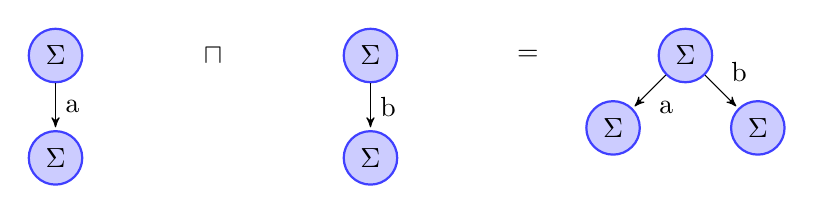
\begin{tikzpicture}[node distance=1.3cm,>=stealth',bend angle=45,auto]
  \tikzstyle{place}=[circle,thick,draw=blue!75,fill=blue!20,minimum size=6mm]
  \tikzstyle{red place}=[place,draw=red!75,fill=red!20]
  \tikzstyle{transition}=[rectangle,thick,draw=black!75,
  			  fill=black!20,minimum size=4mm]
  \tikzstyle{every label}=[red]
  \begin{scope}
    \node [place] (w1) {$\Sigma$};
    \node [place] (e1) [below of=w1] {$\Sigma$}
      edge [pre]  node[swap] {a}                 (w1);      
  \end{scope}
  \begin{scope}[xshift=4cm]
    \node [place] (w1) {$\Sigma$};
    \node [place] (e1) [below of=w1] {$\Sigma$}
      edge [pre]  node[swap] {b}                 (w1);      
  \end{scope} 
  \begin{scope}[xshift=8cm]
    \node [place] (w1) {$\Sigma$};
    \node [place] (e1) [below left of=w1] {$\Sigma$}
      edge [pre]  node[swap] {a}                 (w1);      
    \node [place] (e1) [below right of=w1] {$\Sigma$}
      edge [pre]  node[swap] {b}                 (w1);      
  \end{scope}
  \draw (2,0) node {$\sqcap$};
  \draw (6,0) node {$=$};
\end{tikzpicture}
\caption{Example of $\sqcap$.}
\end{figure}

\begin{figure}[H]
\centering
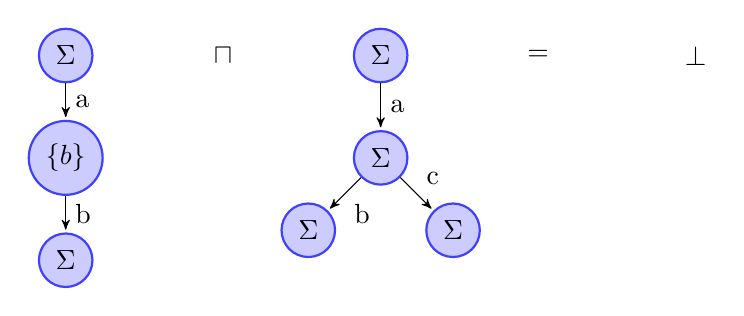
\begin{tikzpicture}[node distance=1.3cm,>=stealth',bend angle=45,auto]
  \tikzstyle{place}=[circle,thick,draw=blue!75,fill=blue!20,minimum size=6mm]
  \tikzstyle{red place}=[place,draw=red!75,fill=red!20]
  \tikzstyle{transition}=[rectangle,thick,draw=black!75,
  			  fill=black!20,minimum size=4mm]
  \tikzstyle{every label}=[red]
  \begin{scope}
    \node [place] (w1) {$\Sigma$};
    \node [place] (e1) [below of=w1] {$\{b\}$}
      edge [pre]  node[swap] {a}                 (w1);      
    \node [place] (e2) [below of=e1] {$\Sigma$}
      edge [pre]  node[swap] {b}                 (e1);      
  \end{scope}
  \begin{scope}[xshift=4cm]
    \node [place] (w1) {$\Sigma$};
    \node [place] (e1) [below of=w1] {$\Sigma$}
      edge [pre]  node[swap] {a}                 (w1);      
    \node [place] (e2) [below right of=e1] {$\Sigma$}
      edge [pre]  node[swap] {c}                 (e1);      
    \node [place] (e3) [below left of=e1] {$\Sigma$}
      edge [pre]  node[swap] {b}                 (e1);      
  \end{scope} 
  \begin{scope}[xshift=8cm]
    \node (w1) {$\bot$};
  \end{scope}
  \draw (2,0) node {$\sqcap$};
  \draw (6,0) node {$=$};
\end{tikzpicture}
\caption{Example of $\sqcap$.}
\end{figure}

\begin{figure}[H]
\centering
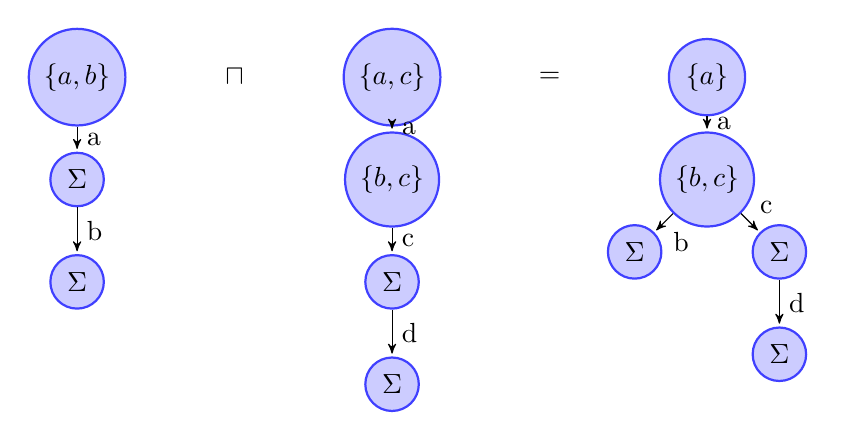
\begin{tikzpicture}[node distance=1.3cm,>=stealth',bend angle=45,auto]
  \tikzstyle{place}=[circle,thick,draw=blue!75,fill=blue!20,minimum size=6mm]
  \tikzstyle{red place}=[place,draw=red!75,fill=red!20]
  \tikzstyle{transition}=[rectangle,thick,draw=black!75,
  			  fill=black!20,minimum size=4mm]
  \tikzstyle{every label}=[red]
  \begin{scope}
    \node [place] (w1) {$\{a,b\}$};
    \node [place] (e1) [below of=w1] {$\Sigma$}
      edge [pre]  node[swap] {a}                 (w1);      
    \node [place] (e2) [below of=e1] {$\Sigma $}
      edge [pre]  node[swap] {b}                 (e1);      
  \end{scope}
  \begin{scope}[xshift=4cm]
    \node [place] (w1) {$\{a,c\}$};
    \node [place] (e1) [below of=w1] {$\{b,c\}$}
      edge [pre]  node[swap] {a}                 (w1);      
    \node [place] (e2) [below of=e1] {$\Sigma $}
      edge [pre]  node[swap] {c}                 (e1);      
    \node [place] (e3) [below of=e2] {$\Sigma $}
      edge [pre]  node[swap] {d}                 (e2);      
  \end{scope} 
  \begin{scope}[xshift=8cm]
    \node [place] (w1) {$\{a\}$};
    \node [place] (e1) [below of=w1] {$\{b, c\} $}
      edge [pre]  node[swap] {a}                 (w1);      
    \node [place] (e2) [below left of=e1] {$\Sigma $}
      edge [pre]  node[swap] {b}                 (e1);      
    \node [place] (e3) [below right of=e1] {$\Sigma $}
      edge [pre]  node[swap] {c}                 (e1);      
    \node [place] (e4) [below of=e3] {$\Sigma $}
      edge [pre]  node[swap] {d}                 (e3);      
  \end{scope}
  \draw (2,0) node {$\sqcap$};
  \draw (6,0) node {$=$};
\end{tikzpicture}
\caption{Example of $\sqcap$. }
\end{figure}

\begin{figure}[H]
\centering
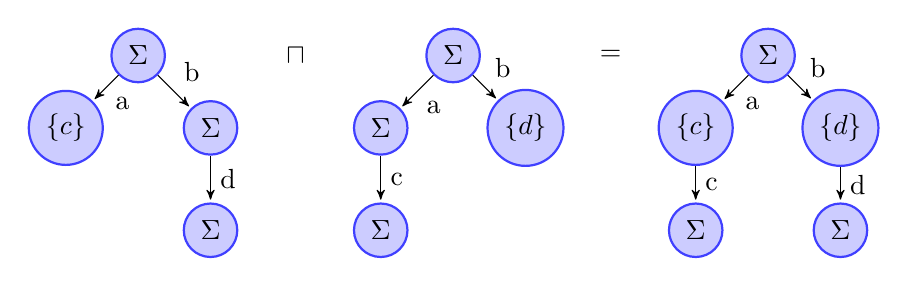
\begin{tikzpicture}[node distance=1.3cm,>=stealth',bend angle=45,auto]
  \tikzstyle{place}=[circle,thick,draw=blue!75,fill=blue!20,minimum size=6mm]
  \tikzstyle{red place}=[place,draw=red!75,fill=red!20]
  \tikzstyle{transition}=[rectangle,thick,draw=black!75,
  			  fill=black!20,minimum size=4mm]
  \tikzstyle{every label}=[red]
  
  \begin{scope}
    \node [place] (w1) {$\Sigma$};
    \node [place] (e1) [below left of=w1] {$\{c\}$}
      edge [pre]  node[swap] {a}                 (w1);      
    \node [place] (e2) [below right of=w1] {$\Sigma$}
      edge [pre]  node[swap] {b}                 (w1);      
    \node [place] (e3) [below of=e2] {$\Sigma$}
      edge [pre]  node[swap] {d}                 (e2);      
  \end{scope}
  
  \begin{scope}[xshift=4cm]
    \node [place] (w1) {$\Sigma$};
    \node [place] (e1) [below left of=w1] {$\Sigma$}
      edge [pre]  node[swap] {a}                 (w1);      
    \node [place] (e2) [below right of=w1] {$\{d\}$}
      edge [pre]  node[swap] {b}                 (w1);      
    \node [place] (e3) [below of=e1] {$\Sigma$}
      edge [pre]  node[swap] {c}                 (e1);      
  \end{scope}
  
  
  \begin{scope}[xshift=8cm]
    \node [place] (w1) {$\Sigma$};
    \node [place] (e1) [below left of=w1] {$\{c\}$}
      edge [pre]  node[swap] {a}                 (w1);      
    \node [place] (e2) [below right of=w1] {$\{d\}$}
      edge [pre]  node[swap] {b}                 (w1);      
    \node [place] (e3) [below of=e1] {$\Sigma$}
      edge [pre]  node[swap] {c}                 (e1);      
    \node [place] (e4) [below of=e2] {$\Sigma$}
      edge [pre]  node[swap] {d}                 (e2);      
  \end{scope}
  
  \draw (2,0) node {$\sqcap$};
  \draw (6,0) node {$=$};
\end{tikzpicture}
\caption{Example of $\sqcap$.}
\end{figure}





\NI Note that by our conventions, $\SIMPL{\phi}$ really returns a
$\MODELEQ$-equivalence class of models.

The only complex case is the clause for $\SIMPL{\phi_1 \AND \phi_2}$,
which uses the $\sqcap$ function, defined as follows, where we assume
that the sets of states in the two models are disjoint.

\begin{eqnarray*}
  \bot \sqcap \MMM  &\ =\ &  \bot  \\
  \MMM \sqcap \bot      & = &  \bot  
     \\
  \MMM \sqcap \MMM'
     & = & 
  \begin{cases}
    \mathsf{merge}(\MMM, \MMM') & \text{if}\ \mathsf{consistent}(\MMM, \MMM') \\
    \bot & \text{else}
  \end{cases}
\end{eqnarray*}

\NI The $\mathsf{consistent}$ predicate is true of models $m$ and $n$ if
the out-transitions on $m$'s root state respect the labelling on $n$'s
root state, and the out-transitions on $n$'s root state respect the
labelling on $m$'s root state. In other words:

\begin{eqnarray*}
  \mathsf{consistent}(\MMM, \MMM') 
     &\ \mbox{ iff }\ & 
  \begin{cases}
    \mathsf{out}(\MMM) \subseteq \mathsf{restriction}(\MMM') \mbox{ and}  \\
    \mathsf{out}(\MMM') \subseteq \mathsf{restriction}(\MMM) 
  \end{cases}
\end{eqnarray*}

\NI Here:

\[
\begin{array}{rcl}
  \mathsf{out}(((S,\rightarrow,\lambda),w)) 
     &\ =\ & \{ a \fOr \exists w' . w \xrightarrow{a} w'\}  \\
  \mathsf{restriction}(((S,\rightarrow,\lambda),w)) 
    & = & 
  \lambda(w) 
\end{array}
\]

\NI Now the $\mathsf{merge}$ function fuses two  models together:
\[
   \mathsf{merge}( ( (S, \rightarrow, \lambda), w),  ( (S', \rightarrow', \lambda'), w')) 
      \ =\ 
   ((S \cup S', \rightarrow \cup \rightarrow'_2, \lambda_2 \cup \lambda'_2), w)
\]
where:
\begin{eqnarray*}
  \rightarrow'_2 &\ =\ & \rightarrow' \mbox{ with } w' \mbox{ replaced by } w  \\
  \lambda_2 & = & \lambda \mbox{ with } w \mapsto \lambda(w) \cap \lambda'(w')  \\
  \lambda'_2 & = & \lambda' \mbox{ with } w' \mbox{ removed } 
\end{eqnarray*}

\NI It is easy to show that $\SIMPL{\cdot}$ has the following properties:

\begin{itemize}

\item $\SIMPL{\phi} \models \phi$.

\item If $\MMM' \models \phi$ and  $\MMM \MODELLEQ \MMM'$ then also  $\MMM \models \phi$.
 
\end{itemize}

\begin{figure}[H]
\centering
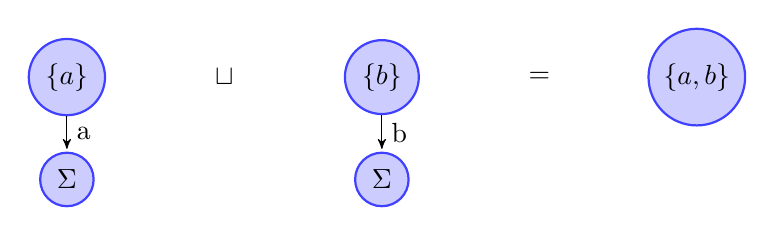
\begin{tikzpicture}[node distance=1.3cm,>=stealth',bend angle=45,auto]
  \tikzstyle{place}=[circle,thick,draw=blue!75,fill=blue!20,minimum size=6mm]
  \tikzstyle{red place}=[place,draw=red!75,fill=red!20]
  \tikzstyle{transition}=[rectangle,thick,draw=black!75,
  			  fill=black!20,minimum size=4mm]
  \tikzstyle{every label}=[red]
  \begin{scope}
    \node [place] (w1) {$\{a\}$};
    \node [place] (e1) [below of=w1] {$\Sigma$}
      edge [pre]  node[swap] {a}                 (w1);      
  \end{scope}
  \begin{scope}[xshift=4cm]
    \node [place] (w1) {$\{b\}$};
    \node [place] (e1) [below of=w1] {$\Sigma$}
      edge [pre]  node[swap] {b}                 (w1);      
  \end{scope}
  \begin{scope}[xshift=8cm]
    \node [place] (w1) {$\{a,b\}$};
  \end{scope}
  \draw (2,0) node {$\sqcup$};
  \draw (6,0) node {$=$};
\end{tikzpicture}
\caption{Example of $\sqcup$}
\end{figure}


\begin{figure}[H]
\centering
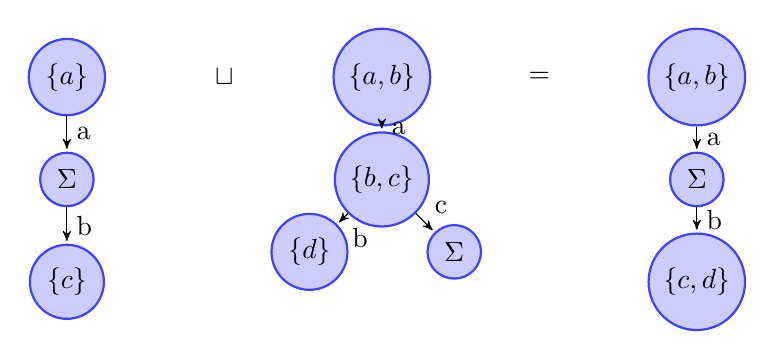
\begin{tikzpicture}[node distance=1.3cm,>=stealth',bend angle=45,auto]
  \tikzstyle{place}=[circle,thick,draw=blue!75,fill=blue!20,minimum size=6mm]
  \tikzstyle{red place}=[place,draw=red!75,fill=red!20]
  \tikzstyle{transition}=[rectangle,thick,draw=black!75,
  			  fill=black!20,minimum size=4mm]
  \tikzstyle{every label}=[red]
  \begin{scope}
    \node [place] (w1) {$\{a\}$};
    \node [place] (e1) [below of=w1] {$\Sigma$}
      edge [pre]  node[swap] {a}                 (w1);      
    \node [place] (e2) [below of=e1] {$\{c\}$}
      edge [pre]  node[swap] {b}                 (e1);      
  \end{scope}
  \begin{scope}[xshift=4cm]
    \node [place] (w1) {$\{a,b\}$};
    \node [place] (e1) [below of=w1] {$\{b,c\}$}
      edge [pre]  node[swap] {a}                 (w1);      
    \node [place] (e2) [below left of=e1] {$\{d\}$}
      edge [pre]  node[swap] {b}                 (e1);      
    \node [place] (e2) [below right of=e1] {$\Sigma$}
      edge [pre]  node[swap] {c}                 (e1);      
  \end{scope} 
  \begin{scope}[xshift=8cm]
    \node [place] (w1) {$\{a,b\}$};
    \node [place] (e1) [below of=w1] {$\Sigma$}
      edge [pre]  node[swap] {a}                 (w1);      
    \node [place] (e2) [below of=e1] {$\{c,d\}$}
      edge [pre]  node[swap] {b}                 (e1);      
  \end{scope}
  \draw (2,0) node {$\sqcup$};
  \draw (6,0) node {$=$};
\end{tikzpicture}
\caption{Example of $\sqcup$}
\end{figure}


\subsubsection{Computing Least Upper Bound ($\sqcup$)}
Define the least upper bound ($\sqcup$) of two models as:
\begin{eqnarray*}
\MMM \sqcup \bot & = & \MMM \\
\bot \sqcup \MMM & = & \MMM \\
(\CAL{L},w) \sqcup (\CAL{L}',w') & = & \mathsf{lub}(\CAL{L}, \CAL{L}', (\MMM_\top, z), \{(w, w', z)\})
\end{eqnarray*}
where $\MMM_\top$ is the topmost model $(\mathcal{W}=\{z\}, \rightarrow=\{\}, \lambda=\{z \mapsto \Sigma\})$ for some state $z$.
$\mathsf{lub}$ takes four parameters: the two eremic transition systems $\CAL{L}$ and $\CAL{L}'$, an accumulator representing the constructed result so far, and a list of state triples (each triple contains one state from each of the two input models plus the state of the accumulated result) to consider next.
It is defined as:
\begin{eqnarray*}
\mathsf{lub}(\CAL{L}, \CAL{L}', \MMM, \{\}) & = & \MMM \\
\mathsf{lub}(\CAL{L}, \CAL{L}', ((\mathcal{W}, \rightarrow, \lambda), y), \{(w,w',x)\} \cup R) & = & \mathsf{lub}(\CAL{L}, \CAL{L}', ((\mathcal{W} \cup \mathcal{W}', \rightarrow \cup \rightarrow', \lambda'), y), R' \cup R\}
\end{eqnarray*}
where:
\begin{eqnarray*}
\{(a_i, w_i, w'_i) \;|\; i = 1 ... n\} & = & \mathsf{sharedT}((\CAL{L},w), (\CAL{L}',w')) \\
\mathcal{W}' & = & \{x_i \;|\; i = 1 ... n\} \\
\rightarrow' & = & \{(x, a_i, x_i) \;|\; i = 1 ... n\} \\
\lambda' & = & \lambda [x \mapsto \lambda(w) \cup \lambda(w)'] \\
R' & = & \{(w_i, w'_i, x_i) \;|\; i = 1 ... n\}
\end{eqnarray*}
Here, $\mathsf{sharedT}$ returns the shared transitions between two models, and is defined as:
\[
\mathsf{sharedT}(((\mathcal{W}, \rightarrow, \lambda),w) ((\mathcal{W}', \rightarrow', \lambda'),w')) =  \{(a, x, x') \;|\; w \xrightarrow{a} x \land w' \xrightarrow{a}' x'\}
\]

\subsubsection{Characteristic formulae}

The function $\SIMPL{\cdot}$ goes from formulae to (equivalence
classes of) models. Now we go the other way: given a(n equivalence class of a) model $\MMM$, we
compute its characteristic formula $\CHAR{m}$. The formula
$\SIMPL{\MMM}$ characterises the model $\MMM$ in the following
sense. \martin{Check that they are true. Proofs?}

\begin{itemize}

\item  $\MMM \models \phi$ implies $\CHAR{\MMM} \models \phi$.

\item  $\MMM \models \CHAR{ \MMM' }$ exactly when $\MMM \MODELLEQ \MMM'$.

\item $\MMM = \BIGLUB \{\MMM' \ |\ \MMM' \models \CHAR{\MMM} \}$.

\end{itemize}

\martin{we must define $\BIGLUB$!}
\richard{It is defined below. Should we move it up?}

\NI This notion of characteristic formula is closely related to
characteristic formulae in Hennessy-Milner logic
\cite{AcetoL:chaforfata} and Hoare logics
\cite{HondaK:descriptive,ChargueraudA:provertcf}. Here is the
definition of $\CHAR{\cdot}$ (again we omit specifying that the function really
returns $\MODELEQ$-equivalence classes of models).

\begin{eqnarray*}
  \CHAR{\bot} &\ =\ & \langle a \rangle \top \AND ! \emptyset  \mbox{ for some symbol }a  \\
  \CHAR{\MMM, w} & = & \mathsf{bang}(\MMM,w) \AND \bigwedge_{(a,w') \in \mathsf{trans}(l,w)} \langle a \rangle \CHAR{\MMM, w'}  
\end{eqnarray*}

\martin{Note that in its current form $\CHAR{\bot}$ defines a
  relation, not a function, because $a$ an vary.}

\NI The functions $\mathsf{bang}(\cdot)$ and $\mathsf{trans}$ on
models are given by the following clauses.

\begin{eqnarray*}
  \mathsf{bang}((S,\rightarrow,\lambda),w) 
     & \ = \ & 
  \begin{cases}
    \top & \mbox{ if } \lambda(w) = \Sigma  \\
    ! \; \lambda(w) & \mbox{ otherwise }  
  \end{cases} \\
  \mathsf{trans}((S,\rightarrow, \lambda),w) & \ = \ & \{(a,w') | w \xrightarrow{a} w' \} 
\end{eqnarray*}

\NI Note that $\CHAR{\MMM}$ is finite if $\MMM$ contains no cycles and if
$\lambda(x)$ is either $\Sigma$ or finite for all states $x$.
Note also that $\SIMPL{\cdot}$ and $\CHAR{\cdot}$ are inverses of each other in that:

\begin{itemize}

\item $\SIMPL{\CHAR{\MMM}} \ = \  \MMM$. \martin{Is this set-theoretic equality?}

\item $\CHAR{\SIMPL{\phi}}$ iff $\phi$.\martin{is this $\vdash$ or $\models$?}

\end{itemize}

\NI We are now ready to prove completeness.  We will show that $\phi
\models \psi$ implies there is a derivation of $\phi \judge \psi$.  Our proof
will make use of two key facts\footnote{These lemmas are proved in the Appendices.}:

\begin{lemma}\label{lemma:completeness:4}
If $\MMM \models \phi$ then $\CHAR{\MMM} \judge \phi$.
\end{lemma}

\begin{lemma}\label{lemma:completeness:5}
For all formulae $\phi$, we can derive $\phi \judge \CHAR{\SIMPL{\phi}}$.
\end{lemma}

\martin{Add short explanation of Lemma \ref{lemma:completeness:4}}.

As to Lemma \ref{lemma:completeness:5}, $\SIMPL{\phi}$ is the simplest model
satisfying $\phi$, and $\CHAR{\MMM}$ is the simplest formula describing
$m$, so $\CHAR{\SIMPL{\phi}}$ is a simplified form of $\phi$. This lemma
states that EL has the inferential capacity to transform any
proposition into its simplified form.

With these two lemmas in hand, the proof of completeness is
straightforward.  Assume $\phi \models \psi$.  Then all models which satisfy
$\phi$ also satisfy $\psi$.  In particular, $\SIMPL{\phi} \models \psi$.  Then
$\CHAR{\SIMPL{\phi}} \judge \psi$ by Lemma \ref{lemma:completeness:4}.  But we
also have, by Lemma \ref{lemma:completeness:5}, $\phi \judge
\CHAR{\SIMPL{\phi}} $.  So by transitivity, we have $\phi \judge \psi$.  


\subsection{The standard translation from  \ELABR{} into 
            first-order logic}\label{standardTranslation}

We now present a translation from EL to first-order logic. We have two
key purposes in mind:

\begin{itemize}

\item To facilitate the comparison between EL and conventional
  first-order logic, to pin down precisely where EL and first-order
  logic differ and where they don't.

\item To enable technology transfer between EL and other logics. We
  are inspired here in particular by the standard translation of modal
  logic into first-order logic \cite{BlackburnP:modlog} which has
  allows the transfer of interesting results such as compactness to
  modal logic, but has also given rise to many interesting concepts in
  first-order logic.  Historically, fragments of first-order logic
  that were studied were defined by quantifier hierarchies. Modal
  logics picks out very different fragments. For example fragments
  closed under bisimulation, guarded fragments, fragments with
  restricted numbers of variables.

\end{itemize}

\begin{FIGURE}
\begin{center}
\includegraphics[width=8cm]{embedding.pdf}
\end{center}
\caption{The standard translation of eremic logic identifies a fragment of
  first-order logic.\textbf{Is it worth keeping this picture?}}\label{figure:embedding}
\end{FIGURE}



\NI We will translate EL into a restricted fragment of first-order
logic (cf.~Figure \ref{figure:embedding}). The first-order signature
$\SSS$ has a nullary predicate $\top$, a family of unary predicates
$\RESTRICT{A}{\cdot}$, one for each finite subset $A \subseteq
\Sigma$, and a family of binary predicates $\ARROW{a}{x}{y}$, one for
each action $a \in \Sigma$.  The intended interpretation is as
follows.

\begin{itemize}

\item The universe is composed of states.

\item The predicate $\top$, which is true everywhere.

\item For each finite $A \subseteq \Sigma$ and each state $s$,  $\RESTRICT{A}{s}$
is true if 
  $\lambda(x) \subseteq A$.

\item A set of two-place predicates $\ARROW{a}{x}{y}$, one for each $a
  \in \Sigma$, where $x$ and $y$ range over states. $\ARROW{a}{x}{y}$
  is true if $x \xrightarrow{a} y$.


\end{itemize}

\NI Note that if $\Sigma$ is infinite, then $\RESTRICT{A}{\cdot}$ and
$\ARROW{a}{\cdot}{\cdot}$ are infinite families of relations.


 Choose two fixed variables $x, y$, let $a$ range over actions in
$\Sigma$, and $A$ over finite subsets of $\Sigma$. Then the restricted
fragment of FOL that is the target of our translation is given by the
following grammar, where $w, z$ range over $x, y$.

\begin{GRAMMAR}
  \phi 
     &\quad ::= \quad&
  \top \fOr \ARROW{a}{w}{z}\fOr \RESTRICT{A}{z} \fOr \phi \AND \psi \fOr \exists x. \phi 
\end{GRAMMAR}

\NI Notice that this fragment of FOL has no negation, disjunction,
implication, or universal quantification. 

The translations $\SEMB{\phi}_x$ and $\SEMB{\phi}_y$ of an EL formula
$\phi$ are given relative to a state, denoted by either $x$ or $y$.

\[
\begin{array}{rclcrcl}
  \SEMB{\top}_x & \ = \ & \top  
     &\quad& 
  \SEMB{\top}_y & \ = \ & \top 
     \\
  \SEMB{\phi \AND \psi}_x & = & \SEMB{\phi}_x \AND \SEMB{\psi}_x  
     && 
  \SEMB{\phi \AND \psi}_y & = & \SEMB{\phi}_y \AND \SEMB{\psi}_y  
     \\
  \SEMB{\langle a \rangle \phi}_x & = & \exists y.(\ARROW{a}{x}{y} \AND \SEMB{\phi}_y)  
     &&
  \SEMB{\langle a \rangle \phi}_y & = & \exists x.(\ARROW{a}{y}{x} \AND \SEMB{\phi}_x)  
     \\
  \SEMB{\fBang A}_x & = & \RESTRICT{A}{x}
     &&
  \SEMB{\fBang A}_y & = & \RESTRICT{A}{y}
\end{array}
\]

\NI The translations on the left and right are identical except for
switching $x$ and $y$. We continue with some example translations.

\[
   \SEMB{\langle a \rangle \top \AND \fBang \{a\}}_x 
      = 
   \exists y.(\ARROW{a}{x}{y} \AND \top ) \AND \RESTRICT{\{a\}}{x}
\]

\martin{Shall we discuss 1 or 2 more? Maybe one that illustrates the
variable switching?}

\NI We now establish the correctness of the encoding. The key issue
issue is that not every first-order model of our first-order signature
corresponds to an eremic model. The problem is that eremic models have
constraints that are not enforced by our signature, e.g.~$s \TRANS{a}
t$ implies that $a \in \lambda(s)$. Such models are 'junk' from the
point of view of \ELABR{}. 

We deal with this problem following ideas from modal logic
\cite{BlackburnP:modlog}: we add a translation $\SEMB{\LLL}$ for
eremic transition systems, and then prove the following theorem.

\begin{theorem}[correspondence theorem]\label{correspondence:theorem:1}
Let $\phi$ be an \ELABR{} formula and $\MMM = (\LLL, s)$ an eremic
model.
\[
   \MMM \models \phi \quad  \text{iff} \quad \SEMB{\LLL} \models_{x \mapsto s} \SEMB{\phi}_x.
\]
And likewise for $\SEMB{\phi}_y$.
\end{theorem}

\NI Before proving the theorem, we define $\SEMB{\LLL}$, which, given
an eremic transition system $\LLL$, produces a corresponding
first-order model for the signature $\SSS$ introduced above. The
translation is simple.

\begin{definition}
Let $\LLL = (S, \rightarrow, \lambda)$ be an eremic transition
system. Clearly $\LLL$ gives rise to an $\SSS$-model $\SEMB{\LLL}$ as
follows.
\begin{itemize}

\item The universe is the set $S$ of states.

\item The relation symbols are interpreted as follows.

  \begin{itemize}

    \item $\top^{\SEMB{\LLL}}$ always holds.

    \item $\mathsf{Restrict}_{A}^{\SEMB{\LLL}} = \{ s \in S\ |\ \lambda(s) \subseteq A\}$.

    \item $\mathsf{Arrow^{\SEMB{\LLL}}}_{a} = \{(s, t) \in S \times S\ |\ s \TRANS{a} t\}$.

  \end{itemize}
\end{itemize}
\end{definition}

\NI We are now ready to prove Theorem \ref{correspondence:theorem:1}.
\begin{proof}
By induction on the structure of $\phi$. The cases $\top$ and $\phi_1
\AND \phi_2$ are straightfoward.  The case $\MAY{a}\psi$ is handeled
as follows.
\begin{eqnarray*}
  \lefteqn{
  \SEMB{\LLL} \models_{x \mapsto s} \SEMB{\MAY{a}\psi}_x}\hspace{5mm} 
     \\
     &\quad \text{iff}\quad &
  \SEMB{\LLL} \models_{x \mapsto s} \exists y.(\ARROW{a}{x}{y} \AND \SEMB{\psi}_y) 
     \\
     &\text{iff}&
  \text{exists}\ t \in S. \SEMB{\LLL} \models_{x \mapsto s, y \mapsto t} \ARROW{a}{x}{y} \AND \SEMB{\psi}_y
     \\
     &\text{iff}&
  \text{exists}\ t \in S. \SEMB{\LLL} \models_{x \mapsto s, y \mapsto t} \ARROW{a}{x}{y} \ \text{and}\ \SEMB{\LLL} \models_{x \mapsto s, y \mapsto t}  \SEMB{\psi}_y
     \\
     &\text{iff}&
  \text{exists}\ t \in S. s \TRANS{a} t \ \text{and}\ \SEMB{\LLL} \models_{x \mapsto s, y \mapsto t}  \SEMB{\psi}_y
     \\
     &\text{iff}&
  \text{exists}\ t \in S. s \TRANS{a} t \ \text{and}\ \SEMB{\LLL} \models_{y \mapsto t}  \SEMB{\psi}_y \qquad (\text{as $x$ is not free in $\psi$})
     \\
     &\text{iff}&
  \text{exists}\ t \in S. s \TRANS{a} t \ \text{and}\ \MMM \models \psi
     \\
     &\text{iff}&
  \MMM \models \MAY{a}\psi  
\end{eqnarray*}

\NI Finally, if $\phi$ is $!A$ the derivation comes straight from the
definitions.
\begin{eqnarray*}
  \SEMB{\LLL} \models_{x \mapsto s} \SEMB{!A}_x
    &\quad \text{iff}\quad &
  \SEMB{\LLL} \models_{x \mapsto s} \RESTRICT{A}{x}
     \\
     &\text{iff}&
  \lambda(s) \subseteq A
     \\
     &\text{iff}&
  \MMM \models\ !A.
\end{eqnarray*}

\end{proof}

\subsection{Compactness}

\NI First-order logic has compactness: a set $S$ of sentences has a
model exactly when every finite subset of $S$ does \cite[Chapter
  4.3]{EndertonHB:matinttl}. What about \ELABR{}? 

We can prove compactness of modal logics using the standard
translation from modal to first-order logic \cite{BlackburnP:modlog}:
we start from a set of modal formula such that each finite subset has
a model. We translate the modal formulae and models to first-order
logic, getting a set of first-order formulae such that each finite
subset has a first-order model. By compactness of first-order logic we
obtain a first-order model of the translated modal formulae. Then we
translate that first-order model back to modal logic, obtaining a
model for the original modal formulae, as required.

Unfortunately we cannot do the same with the translation from \ELABR{}
to first-order logic presented in the previous section. The problem
are the first-order models termed 'junk' above: they do not correspond
to eremic transition systems.  For example the constraint $s
\TRANS{a} t$ implies $a \in \lambda(s)$ might be violated. After all,
merely having signature $\SSS$ is not strong enough a constraint. The
target language of the translation from the previous section is not
expressive enough to have formulae that can guarantee such
constraints.  As we have no reason to belive that the first-order
model whose existence is guarnateed by compactness isn't 'junk', we
cannot use this translation.

We solve this problem with a second translation from \ELABR{} to
first-order logic, this time into a more expressive fragment were we
can constrain first-order models enough to ensure that they always can
be translated back to \ELFULL{}.

The second embedding translates \ELFULL{} to two-sorted first-order
logic. The many-sorted first-order signature $\SSS'$ is given as follows.
\begin{itemize}

\item $\SSS'$ has two sorts, states and actions. 

\item The action constants are given by $\Sigma$. There
are no state constants. 

\item $\SSS'$ has a nullary predicate $\top$.

\item A binary predicate $\ALLOWED{}{\cdot}{\cdot}$. The intended
  meaning of $\ALLOWED{}{x}{a}$ is that at the state denoted by $x$ we
  are allowed to do the action $a$.

\item A ternary predicate $\ARROWTWO{}{\cdot}{\cdot}{\cdot}$ where
  $\ARROWTWO{}{x}{a}{y}$ means that there is a transition from the
  state denoted by $x$ to the state denoted by $y$, and that
  transition is labelled $a$.

\end{itemize}

\NI So $\SSS'$ is a relational signature, i.e.~has no function
symbols.  The intended interpretation should should be
clear.\martin{Phrase this better.}

With the target logic in place, we can now present a second encoding
$\SEMBTWO{\phi}_x$ of \ELABR{} formulae.

\begin{eqnarray*}
  \SEMBTWO{\top}_x & \ = \ & \top
     \\
  \SEMBTWO{\phi \AND \psi}_x & = & \SEMBTWO{\phi}_x \AND \SEMBTWO{\psi}_x
     \\
  \SEMBTWO{\langle a \rangle \phi}_x & = & \exists^{state} y.(\ARROWTWO{}{x}{a}{y} \AND \SEMBTWO{\phi}_y)
     \\
  \SEMBTWO{\fBang A}_x & = & \forall^{action} a.(\ALLOWED{}{x}{a} \IMPLIES a \in A) 
\end{eqnarray*}

\NI Here we use $\exists^{state}$ to indicate that the quantifier ranges
of the sort of states, and $\forall^{action}$ for a quantifier ranging
over actions. The expression $a \in A$ is a shorthand for the
first-order formula
\[
   a = a_1 \OR a = a_2 \OR \cdots \OR a = a_n
\]
assuming that $A = \{a_1, ..., a_n\}$. Since by definition, $A$ is always a finite
set, this is well-defined.

Note that the translation above could be restricted to a two-variable
fragment. Moreover, the standard reduction from many-sorted to
one-sorted first-order logic, does not increase the number of
variables used (although predicates are added, one per sort)
\cite{EndertonHB:matinttl}. For simplicity we will not consider this
matter further.

Before we can state and prove a correspondence theorem for
$\SEMBTWO{\phi}_x$ along the lines of Theorem
\ref{correspondence:theorem:1}, we must also translate eremic
  transition systems $\SEMBTWO{\LLL}$.

\begin{definition}
Let $\LLL = (S, \rightarrow, \lambda)$ be an eremic transition
system. Clearly $\LLL$ gives rise to an $\SSS'$-model $\SEMBTWO{\LLL}$
as follows.
\begin{itemize}

\item For each constant $a \in \Sigma$, $a^{\SEMBTWO{\LLL}}$ is $a$ itself.

\item The sort of states is interpreted by the set $S$.

\item The sort of actions is interpreted by the set $\Sigma$.

\item The relation symbols are interpreted as follows.

  \begin{itemize}

    \item $\top^{\SEMBTWO{\LLL}}$ always holds.

    \item $\ALLOWED{\SEMBTWO{\LLL}}{s}{a}$ holds whenever $a \in \lambda(s)$.

    \item $\ARROWTWO{\SEMBTWO{\LLL}}{s}{a}{t}$ holds whenver $s \TRANS{a} t$.

  \end{itemize}
\end{itemize}
\end{definition}


\begin{theorem}[correspondence theorem]\label{correspondence:theorem:2}
Let $\phi$ be an \ELABR{} formula and $\MMM = (\LLL, s)$ an eremic
model.
\[
   \MMM \models \phi \quad  \text{iff} \quad \SEMBTWO{\LLL} \models_{x \mapsto s} \SEMBTWO{\phi}_x.
\]
\end{theorem}
\begin{proof}
The proof proceeds by induction on the structure of $\phi$ and is
similar to that of Theorem \ref{correspondence:theorem:2}.
The case for the may modality proceeds as follows.  

\begin{alignat*}{2}
  \MMM \models \MAY{a}\phi
     &\quad\text{iff}\quad 
  \text{exists state $t$ with }\ s \TRANS{a} t\ \text{and}\ (\LLL, t) \models \phi \\
     &\quad\text{iff}\quad
  \text{exists state $t$ with }\ s \TRANS{a} t\ \text{and}\ \SEMBTWO{\LLL} \models_{y \mapsto t} \SEMBTWO{\phi}_y &\qquad& \text{by (IH)}\\
     &\quad\text{iff}\quad
  \SEMBTWO{\LLL} \models_{x \mapsto s} \exists^{state} y.(\ARROWTWO{}{x}{a}{y} \AND \SEMBTWO{\phi}_y) \\
     &\quad\text{iff}\quad
   \SEMBTWO{\LLL} \models_{x \mapsto s} \SEMBTWO{\MAY{a}{\phi}}_x
\end{alignat*}
\martin{the 2nd to last inference may need elaboration!}

Finally $!A$.
\begin{alignat*}{2}
  \MMM \models !A
     &\quad\text{iff}\quad
  \lambda (s) \subseteq A \\
      &\quad\text{iff}\quad
  \text{for all }\ a \in \Sigma. a \in A \\
     &\quad\text{iff}\quad
  \SEMBTWO{\LLL} \models_{x \mapsto s} \forall^{action} a. (\ALLOWED{}{x}{a} \IMPLIES a \in A) \\
     &\quad\text{iff}\quad
  \SEMBTWO{\LLL} \models_{x \mapsto s} \SEMBTWO{!A}_x
\end{alignat*}
\martin{again, some steps need elaboration? Also should this go in the appendix?}

\end{proof}

\NI We now use the translation $\SEMBTWO{\phi}_x$ to show that \ELABR{} must also have compactness. The key steps in the proof are
simple, following standard techniques from modal logic
\cite{BlackburnP:modlog}:

\begin{enumerate}

\item Choose a set $T$ of \ELABR{} formulae, such that each finite
  subset $T'$ of $T$ has an eremic model $(\LLL, s)$.

\item Using the translations gives a set $\SEMBTWO{T} =
  \{\SEMBTWO{\phi}\ |\ \phi \in T\}$ of first-order formulae such that
  each finite subset has a first-order model $\SEMBTWO{\LLL}$.

\item By compactness of first-order logic, we can find a first-order
  model $\CAL{M}$ of $\SEMBTWO{T}$.

\item\label{compactness:step:4} Convert $\CAL{M}$ into an eremic transition system
  $\CAL{M}^{\sharp}$ such that $(\CAL{M}^{\sharp}, s) \models T$.

\end{enumerate}

\NI The problematic step is (\ref{compactness:step:4}), for how would
we know that the model $\CAL{M}$ can be converted back to an eremic
transition system? Why should $\CAL{M}$ exhibit admissibility or
well-sizedness?  The mere fact that $\CAL{M}$ is a first-order model
of signature $\SSS'$ is not strong enough to guarantee these
properties.  We deal with this in two ways. To ensure admissibility,
we define a formula that guarantees that models satisfying the formula
are admissible.
\begin{eqnarray*}
   \phi_{admis} 
      & \ =\ &
   \forall^{state} s.\forall^{action} a.\forall^{state} t.( \ARROWTWO{}{s}{a}{t} \IMPLIES \ALLOWED{}{s}{a})
\end{eqnarray*}

\begin{lemma}\label{compactness:lemma:23399}
If $\LLL$ is an eremic transistion system then $\SEMBTWO{\LLL} \models
\phi_{admis}$.
\end{lemma}

\begin{proof}
Straightforward from the definitions.

\end{proof}

\NI We can now add, without changing satisfiability, $\phi_{admis}$ to
any set of first-order formulae that has a model that is the
translation of an eremic model.

%% We deal with the absence of well-sizedness by 

%% First we add a formula $\phi_a$ for each action $a \in \Sigma$.
%% \begin{eqnarray*}
%%    \phi_{a} 
%%       & = &
%%    \exists^{action} c. a = c 
%% \end{eqnarray*}

%% \begin{lemma}\label{compactness:lemma:666}
%% If $\LLL$ is an eremic transistion system then $\SEMBTWO{\LLL} \models
%% \phi_{a}$ for all $a \in \Sigma$.
%% \end{lemma}

%% \begin{proof}
%% Straightforward from the definitions.
%% 
%% \end{proof}

\begin{definition}
Let $\LLL = (S, \rightarrow, \lambda)$ be an eremic transition system
and $X$ a set, condidered to contain actions. The \emph{restriction of
  $\LLL$ to $X$}, written $\LLL \setminus X$ is the eremic model $(S,
\rightarrow', \lambda')$ where $\rightarrow' = \{(s, a, t) \in
\rightarrow \ |\ a \notin X\}$, and for all states $s$ we set:
\[
   \lambda'(s) 
        =
   \begin{cases}
       \lambda(s) \setminus  X & \text{whenever}\ \lambda(s) \neq \Sigma \\
       \Sigma & \text{otherwise}
   \end{cases}
\]

\end{definition}

\begin{lemma}\label{compactness:lemma:1717}
Let $\phi$ be an \ELABR{} formula and $X$ be a set such that no action
occuring in $\phi$ is in $X$. Then:
\[
   (\LLL, s) \models \phi
      \quad\text{iff}\quad
   (\LLL \setminus X, s) \models \phi.
\]
\end{lemma}
\begin{proof}
By straightforward induction on the structure of $\phi$, using the
fact that by assumption $X$ only contains actions not occuring in
$\phi$.  
\end{proof}

\begin{definition}
Let $\CAL{M}$ be a first-order model for the signature $\SSS'$.
We construct an eremic transition system
$\CAL{M}^{\sharp} = (S, \rightarrow, \lambda)$.
\begin{itemize}

\item The actions $\Sigma$ are given by the $\CAL{M}$ interpretation of actions.

\item The states $S$ are given by the $\CAL{M}$ interpretation of states.

\item The reduction relation $s \TRANS{a} t$ holds exactly when
  $\ARROWTWO{\CAL{M}}{s}{a}{t}$.

\item The function $\lambda$ is given by the following clause:
  \[
     \lambda(s) 
        =
     \begin{cases} 
       X & \text{whenever}\ X = \{a \ |\ \ALLOWED{\CAL{M}}{s}{a} \}\ \text{ is finite} \\
       \Sigma & \text{otherwise}
     \end{cases}
  \]

\end{itemize}

\end{definition}

\begin{lemma}
If $\CAL{M}$ be a first-order model for $\SSS'$ such that $\CAL{M}
\models \phi_{admis}$.  Then $\CAL{M}^{\sharp}$ is an eremic
transition system with actions $\Sigma$.
\end{lemma}
\begin{proof}
Immediate from the definitions.

\end{proof}

\begin{theorem}[correspondence theorem]\label{correspondence:theorem:223}
Let $\CAL{M}$ be a first-order model for the signature $\SSS'$ such that
 $\CAL{M} \models \phi_{admis}$.
Then we have for all \ELABR{} formulae $\phi$ with
actions from $\Sigma$:
\[
   \CAL{M} \models_{x \mapsto s} \SEMBTWO{\phi}_x 
        \quad  \text{iff} \quad 
   (\CAL{M}^{\sharp} \setminus X, s) \models \phi.
\]
\end{theorem}
Here $X$ is the set of all elements in the universe of $\CAL{M}$ interpreting
actions that are not in $\Sigma$.
\begin{proof}
The proof proceeds by induction on the structure of $\phi$. \textbf{To do.}
\end{proof}

\begin{definition}
Let $T$ be a set of \ELABR{} formulae, and $\MMM$ an eremic model.  We
write $\MMM \models T$ provided $\MMM \models \phi$ for all $\phi \in
T$.  We say $T$ is \emph{satisfiable} provided $\MMM \models T$.
\end{definition}

\begin{theorem}[Compactness of \ELFULL{}]
A set $T$ of \ELABR{} formulae is satisfiable iff each finite subset of
$T$ is satisfiable.
\end{theorem}
\begin{proof}
For the non-trivial direction, let $T$ be a set of \ELABR{} formulae
such that any finite subset has an eremic model. Define 
\[
  \SEMBTWO{T} 
     \ =\ 
  \{\SEMBTWO{\phi}\ |\ \phi \in T\} 
     \qquad\qquad
  T^*
     \ =\ 
  \SEMBTWO{T} \cup \{\phi_{admis}\} \cup \{ \phi_a\ |\ a \in \Sigma\}
\]
which both are sets of first-order formulae. Clearly each finite subset $T'$ of 
$T^*$ has a first-order model. Why? First consider the subset $T'_{EL}$ of $T'$
which is given as follows.
\[
   T'_{EL} \ =\ \{ \phi \in T\ |\ \SEMBTWO{\phi} \in T' \}
\]
Since $T'_{EL}$ is finite, by assumption there is an eremic model 
\[
   (\LLL, s) \models T'_{EL}
\]
which means we can apply Theorem \ref{correspondence:theorem:223} to get
\[
   \SEMBTWO{\LLL} \models_{x \mapsto s} \SEMBTWO{T'_{EL}},
\]
By construction $T' \setminus \SEMBTWO{T'_{EL}} \subseteq
\{\phi_{admis}\} \cup \{ \phi_a\ |\ a \in \Sigma\}$, so all we have to
show for $T'$ to have a model is that
\[
    \SEMBTWO{\LLL} \models_{x \mapsto s} \{\phi_{admis}\} \cup \{ \phi_a\ |\ a \in \Sigma\},
\]
but that is a direct consequence of Lemma
\ref{compactness:lemma:23399}.  That
means each finite subset of $T^*$ has a model and by appealing to
compactness of first-order many-sorted logic (which is an immediate
consequence of compactenss of one-sorted first-order logic
\cite{EndertonHB:matinttl}), we know there must be a first-order model
$\CAL{M}$ of $T^*$, i.e.
\[
   \CAL{M} \models T^*.
\]
Since $\CAL{M} \models \phi_{admis}$ and $\CAL{M} \models \phi_a$ for all actions $a$, 
we can apply Theorem \ref{correspondence:theorem:223} that also
\[
   (\CAL{M}^{\sharp} \setminus X, s) \models T
\]
where $X$ is the set of all actions in $\CAL{M}^{\sharp}$ that are not
in $\Sigma$. Hence $T$ is satisfiable.
 
\end{proof}






\section{Inference Rules}

\begin{FIGURE}
\begin{RULES}

  \ZEROPREMISERULENAMEDRIGHT
  {
    \phi \judge \phi
  }{Identity}
    \quad
  \ZEROPREMISERULENAMEDRIGHT
  {
    \phi \judge \top
  }{$\top$-Right}
    \quad
  \ZEROPREMISERULENAMEDRIGHT
  {
    \bot \judge \phi
  }{$\bot$-Left}
    \quad
  \TWOPREMISERULENAMEDRIGHT
  {
    \phi \judge \psi
  }
  {
    \psi \judge \xi
  }
  {
    \phi \judge \xi
  }{Transitivity}
    \\\\
  \ONEPREMISERULENAMEDRIGHT
  {
    \phi \judge \psi
  }
  {
    \phi \AND \xi \judge \psi
  }{$\AND$-Left 1}
     \quad
  \ONEPREMISERULENAMEDRIGHT
  {
    \phi \judge \psi
  }
  {
    \xi \AND \phi  \judge \psi
  }{$\AND$-Left 2}
     \quad
  \TWOPREMISERULENAMEDRIGHT
  {
    \phi \judge \psi
  }
  {
    \phi \judge \xi
  }
  {
    \phi \judge \psi \AND \xi
  }{$\AND$-Right}
     \\\\
     \ONEPREMISERULENAMEDRIGHT
     {
       a \notin A
     }
     {
       !A \AND \MAY{a}{\phi} \judge \bot
     }{$\bot$-Right 1}
        \quad
     \ZEROPREMISERULENAMEDRIGHT
     {
       \MAY{a}{\bot} \judge \bot
     }{$\bot$-Right 2}
        \quad
     \TWOPREMISERULENAMEDRIGHT
     {
       \phi \AND \, !A \judge \psi
     }
     {
       A' \subseteq A
     }
     {
       \phi \AND\, !A' \judge \psi
     }{!-Left}
     \\\\
     \TWOPREMISERULENAMEDRIGHT
     {
       \phi \judge !A
     }
     {
       A \subseteq A'
     }
     {
       \phi \judge!A'
     }{!-Right 1}
     \quad
     \TWOPREMISERULENAMEDRIGHT
     {
       \phi \judge !A
     }
     {
       \phi \judge !B
     }
     {
       \phi \judge !(A \cap B)
     }{!-Right 2}
     \quad
     \ONEPREMISERULENAMEDRIGHT
     {
       \phi \judge \psi
     }
     {
       \MAY{a}{\phi} \judge \MAY{a}{\psi}
     }{Transition Normal}
\end{RULES}
\caption{Proof rules.}\label{figure:elAndBangRules}
\end{FIGURE}


\NI We now present the inference rules for \ELFULL{}. There are no
axioms.

\begin{definition} Judgements are of the following form.
\[
  \phi \judge \psi.
\]
Figure \ref{figure:elAndBangRules} presents all proof rules. 
\end{definition}

\NI Note that $\phi$ and $\psi$ are single formulae, not sequents.  By
using single formulae, we can avoid structural inference rules.  \ELABR{}
proof rules can be grouped in two parts: standard rules and rules
unique to \ELABR{}.  Standard rules are [\RULENAME{Identity}],
[\RULENAME{$\top$-Right}], [\RULENAME{$\bot$-Left}],
[\RULENAME{Transitivity}], [\RULENAME{$\AND$-Left 1}],
[\RULENAME{$\AND$-Left 2}] and [\RULENAME{$\AND$-Right}] hardly need
explanation as they are variants of familiar rules for propositional
logic, see e.g.~\cite{TroelstraAS:basprot,vanDalenD:logstr}.  We now
explain the rules that give EL's its distinctive properties: the
relations betwen $\langle \rangle$, $!$ and $\bot$.

The rule [\RULENAME{$\bot$-Right 1}] axiom captures the core
\emph{exclusion} property of !: for example if $A = \{male, female\}$
then $\MAY{orange}{\phi}$ is incompatible with $!A$. Thus $!A \AND
\MAY{orange}{\phi}$ must be false.

The rule [\RULENAME{$\bot$-Right 2}] expresses that falsity is 'global'
  and cannot be surpressed by prefixing. For example
  $\MAY{orange}{\bot}$ is false, simply because $\bot$ is already
  false.

Relatedly, the rule [\RULENAME{Transition Normal}] enables us to
prefix an inference with a may-modality. For example \martin{add good
  example here.}. Note that it is vital for soundness that $\phi$ in $\phi
\judge \psi$ is a single formula. If we used transitional sequents $\phi_1, ..., \phi_n \judge \psi$,
then the rule
\[
   \ONEPREMISERULE
   {
     \phi_1, ..., \phi_n \judge \psi
   }
   {
     \MAY{a}{\phi_1}, ..., \MAY{a}{\phi_n} \judge \MAY{a}{\psi}
   }
\]
is unsound. \martin{explain why, and why this is significant}. \richard{I think this rule is only unsound if we allow non-determinstic models.}
This
restriction is also in place in \cite{GaySJ:typcalosp} where a
Curry-Howard corrospondence between a fragment of linear logic
\cite{GirardJY:linlog,GirardJY:protyp} and a process calculus is
introduced. We discuss the relationship between EL and linear logic in
general, and linear logic's additive conjunction in Section
\ref{conclusion}.

Note that the logic has no axioms. One reason for a purely rule-based
presentation is the absence of implication in the present fragment of
EL. \martin{explain in more detail!}

\subsection{\RULENAME{!-Left} and \RULENAME{!-Right}}

The rules [\RULENAME{!-Right 1}, \RULENAME{!-Right 2}] jointly express
how the subset relation $\subseteq$ on sets of symbols relates to
provability. Why  don't we need a corresponding rule \RULENAME{!-Left} for
strengthening $!$ on the left hand side?
\[
   \TWOPREMISERULENAMEDRIGHT
     {
       \phi \AND \, !A \judge \psi
     }
     {
       A' \subseteq A
     }
     {
       \phi \AND\, !A' \judge \psi
     }{!-Left}
\]
The reason is that [\RULENAME{!-Left}] can be derived as follows.
\begin{center}
  \AxiomC{$\phi \AND\, !A'  \judge  \phi \AND\, !A'$}
  \AxiomC{$A' \subseteq A$}
  \LeftLabel{\RULENAME{!-Right 1}}
  \BinaryInfC{$\phi \AND\, !A'  \judge  \phi \AND\, !A$}
  \AxiomC{$\phi \AND\, !A  \judge  \psi$}
  \LeftLabel{\RULENAME{Transitivity}}
  \BinaryInfC{$\phi \AND\, !A'  \judge  \psi$}
  \DisplayProof
\end{center}

\NI Readers familiar with object-oriented programming will recognise
[\RULENAME{!-Left}] as contra-variant subtyping and [\RULENAME{!-Right
    1}] as covariant subtyping. Honda \cite{HondaK:thetypftpc}
develops a full theory of subtyping based on similar ideas.  All three
rules embody the intuition that whenever $A \subseteq A'$ then
asserting that $!A'$ is as strong as, or a stronger statement than
$!A$. [\RULENAME{!-Left}] simply states that we can always strengthen
our premise, while [\RULENAME{!-right 1}] allows us to weaken the
premise.

\subsection{Example inferences}
We prove that we can use $\phi \AND \psi  \judge  \xi$ to derive $\MAY{a} \phi \land \MAY{a} \psi \judge \MAY{a} \xi$:
\begin{center}
  \AxiomC{$\phi \AND \psi  \judge  \xi$}
  \LeftLabel{\RULENAME{Transition Normal}}
  \UnaryInfC{$\MAY{a} (\phi \AND \psi)  \judge  \MAY{a} \xi$}
  \AxiomC{$\MAY{a} \phi \land \MAY{a} \psi \judge \MAY{a} \phi \land \MAY{a} \psi$}
  \LeftLabel{\RULENAME{Determinism}}
  \UnaryInfC{$\MAY{a} \phi \land \MAY{a} \psi \judge \MAY{a} (\phi \land \psi)$}
  \LeftLabel{\RULENAME{Transitivity}}
  \BinaryInfC{$\MAY{a} \phi \land \MAY{a} \psi \judge \MAY{a} \xi$}
  \DisplayProof
\end{center}
Next, we prove that we can derive $\MAY{a}!\{b,c\} \land \MAY{a}!\{c,d\} \judge \MAY{a}!\{c\}$:
\begin{center}
  \AxiomC{$!\{b,c\} \judge !\{b,c\}$}
  \LeftLabel{\RULENAME{$\land$ Left 1}}
  \UnaryInfC{$!\{b,c\} \land !\{c,d\} \judge !\{b,c\}$}
  \AxiomC{$!\{c,d\} \judge !\{c,d\}$}
  \LeftLabel{\RULENAME{$\land$ Left 2}}
  \UnaryInfC{$!\{b,c\} \land !\{c,d\} \judge !\{c,d\}$}
  \LeftLabel{\RULENAME{! Right 2}}
  \BinaryInfC{$!\{b,c\} \land !\{c,d\} \judge !\{c\}$}
  \LeftLabel{\RULENAME{Transition Normal}}
  \UnaryInfC{$\MAY{a} (!\{b,c\} \land !\{c,d\}) \judge \MAY{a} !\{c\}$}
  \AxiomC{$\MAY{a} !\{b,c\} \land \MAY{a} !\{c,d\} \judge \MAY{a} !\{b,c\} \land \MAY{a} !\{c,d\}$}
  \LeftLabel{\RULENAME{Determinism}}
  \UnaryInfC{$\MAY{a} !\{b,c\} \land \MAY{a} !\{c,d\} \judge \MAY{a} (!\{b,c\} \land !\{c,d\})$}
  \LeftLabel{\RULENAME{Transitivity}}
  \BinaryInfC{$\MAY{a} !\{b,c\} \land \MAY{a} !\{c,d\} \judge \MAY{a}!\{c\}$}
  \DisplayProof
\end{center}
Next, we prove that we can derive $\MAY{a} !\{b\} \land \MAY{a} \MAY{c} \top \judge \MAY{d} \top$:
\begin{center}
  \AxiomC{$!\{b\} \land \MAY{c}\top \judge \bot$}
  \LeftLabel{\RULENAME{Transition Normal}}
  \UnaryInfC{$\MAY{a}(!\{b\} \land \MAY{c}\top) \judge \MAY{a} \bot$}
  \AxiomC{$\MAY{a}!\{b\} \land \MAY{a} \MAY{c}\top \judge \MAY{a}!\{b\} \land \MAY{a} \MAY{c}\top$}
  \LeftLabel{\RULENAME{Determinism}}
  \UnaryInfC{$\MAY{a}!\{b\} \land \MAY{a} \MAY{c}\top \judge \MAY{a}(!\{b\} \land \MAY{c}\top)$}
  \LeftLabel{\RULENAME{Transitivity}}
  \BinaryInfC{$\MAY{a}!\{b\} \land \MAY{a} \MAY{c}\top  \judge \MAY{a} \bot$}  
  \AxiomC{$\MAY{a}\bot \judge \bot$}
  \LeftLabel{\RULENAME{Transitivity}}
  \BinaryInfC{$\MAY{a}!\{b\} \land \MAY{a} \MAY{c}\top  \judge \bot$}  
  \AxiomC{$\bot \judge \MAY{d} \top$}
  \LeftLabel{\RULENAME{Transitivity}}
  \BinaryInfC{$\MAY{a}!\{b\} \land \MAY{a} \MAY{c}\top  \judge  \MAY{d} \top$}    
  \DisplayProof
\end{center}

\subsection{Characteristic formulae}

In order to prove completeness, below, we need the notion of a \emph{characteristic formula} of a model: the simplest (in terms of entailment) formula that describes the model.

The function $\SIMPL{\cdot}$ goes from formulae to (equivalence
classes of) models. Now we go the other way: given a(n equivalence class of a) model $\MMM$, we
compute its characteristic formula $\CHAR{m}$. The formula
$\CHAR{\MMM}$ characterises the model $\MMM$ in the following
sense. \martin{Check that they are true. Proofs?}

\begin{itemize}

\item  $\MMM \models \phi$ implies $\CHAR{\MMM} \models \phi$.

\item  $\MMM \models \CHAR{ \MMM' }$ exactly when $\MMM \MODELLEQ \MMM'$.

\item $\MMM = \BIGLUB \{\MMM' \ |\ \MMM' \models \CHAR{\MMM} \}$.

\end{itemize}

\martin{we must define $\BIGLUB$!}
\richard{It is defined below. Should we move it up?}

\NI This notion of characteristic formula is closely related to
characteristic formulae in Hennessy-Milner logic
\cite{AcetoL:chaforfata} and Hoare logics
\cite{HondaK:descriptive,ChargueraudA:provertcf}. Here is the
definition of $\CHAR{\cdot}$ (again we omit specifying that the function really
returns $\MODELEQ$-equivalence classes of models).

\begin{eqnarray*}
  \CHAR{\bot} &\ =\ & \langle a \rangle \top \AND ! \emptyset  \mbox{ for some fixed symbol }a \in \Sigma  \\
  \CHAR{\MMM, w} & = & \mathsf{bang}(\MMM,w) \AND \bigwedge_{w \xrightarrow{a} w'} \langle a \rangle \CHAR{\MMM, w'}  
\end{eqnarray*}

\NI Note that $\bot$ requires a particular symbol $a \in \Sigma$. This is why we required, in Section \ref{elsyntax}, that $\Sigma$ is non-empty.

\NI The functions $\mathsf{bang}(\cdot)$ and $\mathsf{trans}$ on
models are given by the following clauses.

\begin{eqnarray*}
  \mathsf{bang}((S,\rightarrow,\lambda),w) 
     & \ = \ & 
  \begin{cases}
    \top & \mbox{ if } \lambda(w) = \Sigma  \\
    ! \; \lambda(w) & \mbox{ otherwise }  
  \end{cases} \\
\end{eqnarray*}

\NI Note that $\CHAR{\MMM}$ is finite if $\MMM$ contains no cycles and if
$\lambda(x)$ is either $\Sigma$ or finite for all states $x$.
Note also that $\SIMPL{\cdot}$ and $\CHAR{\cdot}$ are inverses of each other in that:

\begin{itemize}

\item $\SIMPL{\CHAR{\MMM}} \ = \  \MMM$. \martin{Is this set-theoretic equality?}

\item $\CHAR{\SIMPL{\phi}}$ iff $\phi$.\martin{is this $\vdash$ or $\models$?}

\end{itemize}


\subsection{Soundness and Completeness}

\begin{theorem}\label{theorem:elAndBang:soundComplete}
The rules in Figure \ref{figure:elAndBangRules} are sound and complete:
\begin{enumerate}

\item\label{theorem:elAndBang:sound} (Soundness) $\phi \judge \psi$ implies $\phi \models \psi$.

\item\label{theorem:elAndBang:complete} (Completeness) $\phi \models \psi$ implies $\phi \judge \psi$.

\end{enumerate}
\end{theorem}

\NI Soundness is immediate from the definitions. Completeness is
proved below. 

\begin{definition}
We write $\phi_1, ...,
\phi_n \judge \psi$ whenever $\BIGAND_{i}\phi_i \judge \psi$.  For
arbitrary sets $\Gamma$ of formulae, we write $\Gamma \judge \psi$
provided there are $\phi_1, ..., \phi_n \in \Gamma$ such that $\phi_1,
..., \phi_n \judge \psi$.
\end{definition}

\begin{corollary}
The rules in Figure \ref{figure:elAndBangRules} are sound and complete:
\begin{enumerate}

\item(Soundness) $\Gamma \judge \psi$ implies $\Gamma \models \psi$.

\item (Completeness) $\Gamma \models \psi$ implies $\Gamma \judge \psi$.

\end{enumerate}
\end{corollary}

\begin{proof}
For soundness assume that $\MMM$ is a model with $\MMM \models
\Gamma$.  We know that $\Gamma \judge \psi$ means that we can find a
finite number of formulae $\phi_i \in \Gamma$ with $\AND_i \phi \judge
\psi$.  By soundness then also $\AND_i \phi \models \psi$, hence
clearly $\Gamma \models \psi$.

\NI To prove completeness,  we will show that $\phi
\models \psi$ implies there is a derivation of $\phi \judge \psi$.  Our proof
will make use of two key facts (proved in Sections \ref{prooflemma4} and \ref{prooflemma5} below):

\begin{lemma}\label{lemma:completeness:4}
If $\MMM \models \phi$ then $\CHAR{\MMM} \judge \phi$.
\end{lemma}

\begin{lemma}\label{lemma:completeness:5}
For all formulae $\phi$, we can derive $\phi \judge \CHAR{\SIMPL{\phi}}$.
\end{lemma}

Lemma \ref{lemma:completeness:4} states that, if $\phi$ is satisfied by a model, then there is a proof that the characteristic formula describing that model entails $\phi$.

As to Lemma \ref{lemma:completeness:5}, $\SIMPL{\phi}$ is the simplest model
satisfying $\phi$, and $\CHAR{\MMM}$ is the simplest formula describing
$m$, so $\CHAR{\SIMPL{\phi}}$ is a simplified form of $\phi$. This lemma
states that EL has the inferential capacity to transform any
proposition into its simplified form.

With these two lemmas in hand, the proof of completeness is
straightforward.  Assume $\phi \models \psi$.  Then all models which satisfy
$\phi$ also satisfy $\psi$.  In particular, $\SIMPL{\phi} \models \psi$.  Then
$\CHAR{\SIMPL{\phi}} \judge \psi$ by Lemma \ref{lemma:completeness:4}.  But we
also have, by Lemma \ref{lemma:completeness:5}, $\phi \judge
\CHAR{\SIMPL{\phi}} $.  So by transitivity, we have $\phi \judge \psi$.  

\end{proof}

\subsection{Proof of Lemma \ref{lemma:completeness:4}}
\label{prooflemma4}
If $\MMM\models \phi$ then $\CHAR{\MMM} \judge \phi$.

\NI We proceed by induction on $\phi$.

\martin{no need to number cases if numbers are not referred to later.}
\setcounter{mycase}{0}

\begin{mycase}
$\phi$ is $\top$
\end{mycase}
Then we can prove  $ \CHAR{\MMM} \judge \phi$ immediately using axiom {\bf $\top$ Right}.

\begin{mycase}
$\phi$ is $\psi \AND \psi'$
\end{mycase}
By the induction hypothesis, $  \CHAR{\MMM} \judge \psi$ and $  \CHAR{\MMM} \judge \psi'$.
The proof of $  \CHAR{\MMM} \judge \psi \AND \psi'$ follows immediately using {\bf $\AND$ Right}.

\begin{mycase}
$\phi$ is $\langle a \rangle \psi$
\end{mycase}
If $\MMM \models \langle a \rangle \psi$, then either $\MMM = \bot$ or $\MMM$ is a  model of the form $(\CAL{L},w)$.
\begin{subcase}
$\MMM = \bot$
\end{subcase}
In this case, $  \CHAR{\MMM} =  \CHAR{\bot} = \bot$. (Recall, that we are overloading $\bot$ to mean both the  model at the bottom of our lattice and a formula (such as $\langle s \rangle \top \AND !\{\}$) which is always false).
In this case, $  \CHAR{\bot} \judge  \langle a \rangle \psi$ using {\bf $\bot$ Left}.

\begin{subcase}
 $m$ is a  model of the form $(\CAL{L},w)$
 \end{subcase}
Given $\MMM \models \langle a \rangle \psi$, and that $\MMM$ is a  model of the form $(\CAL{L},w)$, we know that:
\[
(\CAL{L},w) \models \langle a \rangle \psi
\]
From the satisfaction clause for $\langle a \rangle$, it follows that:
\[
\exists w' \mbox{ such that } w \xrightarrow{a} w' \mbox { and } (\CAL{L},w') \models \psi
\]
By the induction hypothesis:
\[
 \CHAR{(\CAL{L},w')} \judge \psi
\]
Now by {\bf Transition Normal}:
\[
\langle a \rangle  \CHAR{(\CAL{L},w')} \judge \langle a \rangle \psi
\]
Using repeated application of {\bf $\AND$ Left}, we can show:
\[
 \CHAR{(\CAL{L},w)} \judge \langle a \rangle  \CHAR{(\CAL{L},w')}
\]
Finally, using {\bf Transitivity}, we derive:
\[
 \CHAR{(\CAL{L},w)} \judge  \langle a \rangle \psi
\]
\begin{mycase}
$\phi$ is $\fBang \psi$
\end{mycase}
If $(\CAL{L},w) \models \fBang A$, then $\lambda(w) \subseteq A$.
Then $ \CHAR{(\CAL{L},w)} = ! \; \lambda(w) \AND \phi$.
Now we can prove $! \; \lambda(w) \AND \phi \judge \fBang A$ using  {\bf $!$ Right 1} and repeated applications of {\bf $\AND$ Left}.


\subsection{Proof of Lemma \ref{lemma:completeness:5}}
\label{prooflemma5}

Now we prove Lemma \ref{lemma:completeness:5}: 
For all formulae $\phi$, we can derive $\phi \judge \CHAR{\SIMPL{\phi}}$.

\begin{proof}
Induction on $\phi$.

\setcounter{mycase}{0}

\begin{mycase}
$\phi$ is $\top$
\end{mycase}
Then we can prove  $\top \judge \top$ using either {\bf $\top$ Right} or {\bf Identity}.

\begin{mycase}
$\phi$ is $\psi \AND \psi'$
\end{mycase}
By the induction hypothesis, $\psi \judge  \CHAR{\SIMPL{\psi}}$ and $\psi' \judge  \CHAR{\SIMPL{\psi'}}$.
Using {\bf $\AND$ Left} and {\bf $\AND$ Right}, we can show:
\[
\psi \AND \psi' \judge  \CHAR{\SIMPL{\psi}} \AND  \CHAR{\SIMPL{\psi'}}
\]
Lemma \ref{final_completeness_lemma}, proven below, states that, for all acyclic models $\MMM$ and $\MMM_2$:
\[
  \CHAR{\MMM} \AND  \CHAR{\MMM_2} \judge  \CHAR{\MMM \sqcap \MMM_2}
\]
From Lemma \ref{final_completeness_lemma} (substituting $\SIMPL{\psi}$ for $\MMM$ and $\SIMPL{\psi'}$ for $\MMM_2$, and noting that $\SIMPL{}$ always produces acyclic models), it follows that:
\[
 \CHAR{\SIMPL{\psi}} \AND  \CHAR{\SIMPL{\psi'}} \judge  \CHAR{\SIMPL{\psi \AND \psi'}}
\]
Our desired result follows using {\bf Transitivity}.

\begin{mycase}
$\phi$ is $\langle a \rangle \psi$
\end{mycase}
By the induction hypothesis, $\psi \judge  \CHAR{\SIMPL{\psi}}$.
Now there are two sub-cases to consider, depending on whether or not $ \CHAR{\SIMPL{\psi}} = \bot$.
\begin{subcase}
$ \CHAR{\SIMPL{\psi}} = \bot$
\end{subcase}
In this case, $ \CHAR{\SIMPL{\langle a \rangle \psi}}$ also equals $\bot$. 
By the induction hypothesis:
\[
\psi \judge \bot
\]
By {\bf Transition Normal}:
\[
\langle a \rangle \psi \judge \langle a \rangle \bot
\]
By {\bf Bottom Right 2}:
\[
\langle a \rangle \bot \judge \bot
\]
The desired proof that:
\[
\langle a \rangle \psi \judge \bot
\]
follows by {\bf Transitivity}.
\begin{subcase}
$ \CHAR{\SIMPL{\psi}} \neq \bot$
\end{subcase}
By the induction hypothesis, $\psi \judge  \CHAR{\SIMPL{\psi}}$.
So, by {\bf Transition Normal}:
\[
\langle a \rangle \psi \judge \langle a \rangle  \CHAR{\SIMPL{\psi}}
\]
The desired conclusion follows from noting that:
\[
 \langle a \rangle  \CHAR{\SIMPL{\psi}} =  \CHAR{\SIMPL{\langle a \rangle \psi}}
 \]
 \begin{mycase}
$\phi$ is $\fBang A$
\end{mycase}
If $\phi$ is $\fBang A$, then $  \CHAR{\SIMPL{\phi}}$ is $\fBang A \AND \top$.
We can prove $\fBang A \judge \fBang A \AND \top$ using {\bf $\AND$ Right}, {\bf $\top$ Right} and {\bf Identity}.
\end{proof}

\subsection{Proof of Lemma \ref{final_completeness_lemma}}
\label{prooflemma6}
Finally, to fill the hole in Case 2 of Lemma \ref{lemma:completeness:5} above, we need to show that:
\begin{lemma}
\label{final_completeness_lemma}
For all acyclic models $\MMM$ and $\MMM_2$, $  \CHAR{\MMM} \AND  \CHAR{\MMM_2} \judge  \CHAR{\MMM \sqcap \MMM_2}$.
\end{lemma}

\begin{proof}

There are two cases to consider, depending on whether or not $(\MMM \sqcap \MMM_2) = \bot$.

\setcounter{mycase}{0}

\begin{mycase}
$(\MMM \sqcap \MMM_2) = \bot$
\end{mycase}
If $(\MMM \sqcap \MMM_2) = \bot$, there are three possibilities:
\begin{itemize}
\item
$\MMM = \bot$
\item
$\MMM_2 = \bot$
\item
Neither $\MMM$ nor $\MMM_2$ are $\bot$, but together they are incompatible. 
\end{itemize}
If either $\MMM$ or $\MMM_2$ is $\bot$, then the proof is a simple application of {\bf Identity} followed by {\bf $\AND$ Left}.

Next, let us consider the case where neither $\MMM$ nor $\MMM_2$ are $\bot$, but together they are incompatible.
Let $\MMM = (\mathcal{L}, w_1)$ and $\MMM' = (\mathcal{L}', w'_1)$.
If $\MMM \sqcap \MMM_2 = \bot$, then there is a finite sequence of actions $a_1, ..., a_{n-1}$ such that both $\MMM$ and $\MMM'$ satisfy $\MAY{a_1} ... \MAY{a_{n-1}}\top$, but they disagree about the node labelling on the final node of this chain. In other words, there is a $b$-transition from the final node in $\MMM$ which is ruled-out by the $\lambda'$ node labelling in $\MMM'$. So there is a set of states $w_1, ..., w'_1, ...$ and a finite set $X$ of actions such that:
\begin{eqnarray*}
w_1 \xrightarrow{a_1} w_2 \xrightarrow{a_2} ... \xrightarrow{a_{n-1}} w_n \\
w_1' \xrightarrow{a_1} w'_2 \xrightarrow{a_2} ... \xrightarrow{a_{n-1}} w'_n \\
w_n \xrightarrow{b} w_{n+1} \\
\lambda'(w'_n) = X \text{ with } b \notin X
\end{eqnarray*}
Now it is easy to show, using {\bf $\AND$ Left}, that
\begin{eqnarray*}
\CHAR{\mathsf{\MMM}} \judge \MAY{a_1} ... \MAY{a_{n-1}} \MAY{b} \top \\
\CHAR{\mathsf{\MMM'}} \judge \MAY{a_1} ... \MAY{a_{n-1}} \fBang X
\end{eqnarray*}
Now using {\bf $\AND$ Left} and {\bf $\AND$ Right}:
\[
\CHAR{\mathsf{\MMM}} \land \CHAR{\mathsf{\MMM}'} \judge  \MAY{a_1} ... \MAY{a_{n-1}} \MAY{b} \top \land  \judge \MAY{a_1} ... \MAY{a_{n-1}} \fBang X
\]
Now using {\bf Determinism}:
\[
\CHAR{\mathsf{\MMM}} \land \CHAR{\mathsf{\MMM}'} \judge  \MAY{a_1} ... \MAY{a_{n-1}} (\MAY{b} \top \land \fBang X)
\]
Now, using {\bf $\bot$ Right 1}:
\[
\MAY{b} \top \land \fBang X \judge \bot
\]
Using $n-1$ applications of  {\bf $\bot$ Right 2}:
\[
\MAY{a_1} ... \MAY{a_{n-1}} (\MAY{b} \top \land \fBang X) \judge \bot
\]
Finally, using {\bf Transitivity}, we derive:
\[
\CHAR{\mathsf{\MMM}} \land \CHAR{\mathsf{\MMM}'} \judge \bot
\]
\begin{mycase}
$(\MMM \sqcap \MMM_2) \neq \bot$
\end{mycase}
From the construction of $\mathsf{merge}$, if $\MMM$ and $\MMM'$ are acyclic, then $\MMM \sqcap \MMM'$ is also acyclic.
If $\MMM \sqcap \MMM'$ is acyclic, then $\CHAR{\MMM \sqcap \MMM'}$ is equivalent to a set $\Gamma$ of sentences of one of two forms:
\begin{eqnarray*}
\MAY{a_1} ... \MAY{a_n} \top \\
\MAY{a_1} ... \MAY{a_n} ! X
\end{eqnarray*}

\begin{figure}[H]
\centering
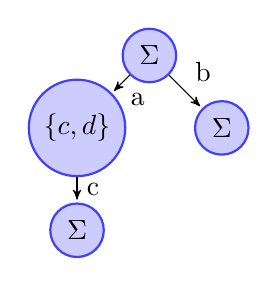
\begin{tikzpicture}[node distance=1.3cm,>=stealth',bend angle=45,auto]
  \tikzstyle{place}=[circle,thick,draw=blue!75,fill=blue!20,minimum size=6mm]
  \tikzstyle{red place}=[place,draw=red!75,fill=red!20]
  \tikzstyle{transition}=[rectangle,thick,draw=black!75,
  			  fill=black!20,minimum size=4mm]
  \tikzstyle{every label}=[red]
    
  \begin{scope}
    \node [place] (w1) {$\Sigma$};
    \node [place] (e1) [below left of=w1] {$\{c,d\}$}
      edge [pre]  node[swap] {a}                 (w1);      
    \node [place] (e2) [below right of=w1] {$\Sigma$}
      edge [pre]  node[swap] {b}                 (w1);      
    \node [place] (e3) [below of=e1] {$\Sigma$}
      edge [pre]  node[swap] {c}                 (e1);      
  \end{scope}
    
\end{tikzpicture}
\caption{Example of $\sqcap$}
\label{setofpaths}
\end{figure}
For example, if $\MMM \sqcap \MMM'$ is as in Figure \ref{setofpaths}, then 
\[
\CHAR{\MMM \sqcap \MMM'} = \MAY{a}(\fBang \{c,d\} \land \MAY{c} \top) \land \MAY{b} \top
\]
This is equivalent to the set $\Gamma$ of sentences:
\begin{eqnarray*}
\MAY{a}\MAY{c} \top \\
\MAY{b} \top \\
\MAY{a}\fBang\{c,d\}
\end{eqnarray*}
Now using {\bf $\AND$ Right} and {\bf Determinism} we can show that
\[
\bigwedge_{\phi \in \Gamma} \phi \judge \CHAR{\MMM \sqcap \MMM'}
\]
We know that for all $\phi \in \Gamma$
\[
\MMM \sqcap \MMM' \models \phi
\]
We just need to show that:
\[
\CHAR{\MMM} \land \CHAR{\MMM'} \judge \phi
\]
Take any $\phi \in \Gamma$ of the form $\MAY{a_1} ... \MAY{a_n} ! X$ for some finite $X \subseteq \Sigma$. (The case where $\phi$ is of the form $\MAY{a_1} ... \MAY{a_n} \top$ is very similar, but simpler).
If $\MMM \sqcap \MMM' \models \MAY{a_1} ... \MAY{a_n} ! X$ then either:
\begin{enumerate}
\item
$\MMM \models \MAY{a_1} ... \MAY{a_n} ! X$ but $\MMM' \nvDash \MAY{a_1} ... \MAY{a_n} \top$
\item
$\MMM' \models \MAY{a_1} ... \MAY{a_n} ! X$ but $\MMM \nvDash \MAY{a_1} ... \MAY{a_n} \top$
\item
$\MMM \models \MAY{a_1} ... \MAY{a_n} ! X_1$ and $\MMM' \models \MAY{a_1} ... \MAY{a_n} ! X_2$ and $X_1 \cap X_2 \subseteq X$
\end{enumerate}
In the first two cases, showing $\CHAR{\MMM} \land \CHAR{\MMM'} \judge \phi$ is just a matter of repeated application of   {\bf $\AND$ Left} and {\bf $\AND$ Right}.
In the third case, let $\MMM = (\mathcal{L}, w_1)$ and $\MMM' = (\mathcal{L}', w'_1)$.
If $\MMM \models \MAY{a_1} ... \MAY{a_n} ! X_1$ and $\MMM' \models \MAY{a_1} ... \MAY{a_n} ! X_2$ then there exists sequences $w_1, ..., w_{n+1}$ and $w'_1, ..., w'_{n+1}$ of states such that
\begin{eqnarray*}
w_1 \xrightarrow{a_1} ... \xrightarrow{a_n} w_{n+1} \\
w'_1 \xrightarrow{a_1} ... \xrightarrow{a_n} w'_{n+1} \\
\lambda(w_{n+1}) \subseteq X_1 \\
\lambda'(w'_{n+1}) \subseteq X_2 \\
\end{eqnarray*}
Now from the definition of $\CHAR{}$:
\begin{eqnarray*}
\CHAR{(\mathcal{L}, w_{n_1})} \judge \fBang X_1 \\
\CHAR{(\mathcal{L}', w'_{n_1})} \judge \fBang X_2
\end{eqnarray*}
Now using {\bf \fBang Right 2}:
\[
\CHAR{(\mathcal{L}, w_{n_1})} \land \CHAR{(\mathcal{L}', w'_{n_1})} \judge \fBang (X_1 \cap X_2)
\]
Using {\bf \fBang Right 1}:
\[
\CHAR{(\mathcal{L}, w_{n_1})} \land \CHAR{(\mathcal{L}', w'_{n_1})} \judge \fBang X
\]
Using $n$ applications of {\bf Transition Normal}:
\[
\MAY{a_1} ... \MAY{a_n} (\CHAR{(\mathcal{L}, w_{n_1})} \land \CHAR{(\mathcal{L}', w'_{n_1})}) \judge \MAY{a_1} ... \MAY{a_n} \fBang X
\]
Finally, using $n$ applications of {\bf Determinism}:
\[
\CHAR{ (\mathcal{L}, w_1)} \land \CHAR{ (\mathcal{L}', w'_1)} \judge \MAY{a_1} ... \MAY{a_n} (\CHAR{(\mathcal{L}, w_{n_1})} \land \CHAR{(\mathcal{L}', w'_{n_1})})
\]
So, by {\bf Transitivity}
\[
\CHAR{\MMM} \land \CHAR{\MMM'} \judge \MAY{a_1} ... \MAY{a_n} \fBang X
\]
\end{proof}

\section{Compactness and the standard translation to first-order logic }
\label{compactness}

This section studies two embeddings of \cathoristic{} into first-order
logic. The second embedding is used to prove that \cathoristic{} satisfies compactness.

\subsection{Translating from  cathoristic to
            first-order logic}\label{standardTranslation}

When we study how a logic embeds into other logics, it casts a new light
on the logic that is the target of the embedding. 
A good example is the standard translation of modal into first-order logic: the translation
produces various fragments: the finite variable
fragments, the fragment closed under bisimulation, and guarded fragments.
These fragments have been investigated heavily, as they have unusual properties not shared by the whole of \fol. 
Translations also enable us to
push techniques, constructions and results between logics.

%\begin{FIGURE}
\begin{center}
\includegraphics[width=8cm]{embedding.pdf}
\end{center}
\caption{The standard translation of eremic logic identifies a fragment of
  first-order logic.\textbf{Is it worth keeping this picture?}}\label{figure:embedding}
\end{FIGURE}



In this section, we translate \cathoristic{} into a restricted fragment of
first-order logic.

\begin{definition}
The first-order signature $\SSS$ has a nullary predicate $\top$, a
family of unary predicates $\RESTRICT{A}{\cdot}$, one for each finite
subset $A \subseteq \Sigma$, and a family of binary predicates
$\ARROW{a}{x}{y}$, one for each action $a \in \Sigma$. 

\end{definition}

\NI The intended interpretation is as follows.

\begin{itemize}

\item The universe is composed of states.

\item The predicate $\top$, which is true everywhere.

\item For each finite $A \subseteq \Sigma$ and each state $s$,  $\RESTRICT{A}{s}$
is true if 
  $\lambda(x) \subseteq A$.

\item A set of two-place predicates $\ARROW{a}{x}{y}$, one for each $a
  \in \Sigma$, where $x$ and $y$ range over states. $\ARROW{a}{x}{y}$
  is true if $x \xrightarrow{a} y$.


\end{itemize}

\NI If $\Sigma$ is infinite, then $\RESTRICT{A}{\cdot}$ and
$\ARROW{a}{\cdot}{\cdot}$ are infinite families of relations.

\begin{definition}
 Choose two fixed variables $x, y$, let $a$ range over actions in
$\Sigma$, and $A$ over finite subsets of $\Sigma$. Then the restricted
fragment of FOL that is the target of our translation is given by the
following grammar, where $w, z$ range over $x, y$.

\begin{GRAMMAR}
  \phi 
     &\quad ::= \quad&
  \top \fOr \ARROW{a}{w}{z}\fOr \RESTRICT{A}{z} \fOr \phi \AND \psi \fOr \exists x. \phi 
\end{GRAMMAR}

\end{definition}

\NI This fragment has no negation, disjunction, implication, or
universal quantification.

\begin{definition}
The translations $\SEMB{\phi}_x$ and $\SEMB{\phi}_y$ of cathoristic formula 
$\phi$ are given relative to a state, denoted by either $x$ or $y$.

\[
\begin{array}{rclcrcl}
  \SEMB{\top}_x & \ = \ & \top  
     &\quad& 
  \SEMB{\top}_y & \ = \ & \top 
     \\
  \SEMB{\phi \AND \psi}_x & = & \SEMB{\phi}_x \AND \SEMB{\psi}_x  
     && 
  \SEMB{\phi \AND \psi}_y & = & \SEMB{\phi}_y \AND \SEMB{\psi}_y  
     \\
  \SEMB{\langle a \rangle \phi}_x & = & \exists y.(\ARROW{a}{x}{y} \AND \SEMB{\phi}_y)  
     &&
  \SEMB{\langle a \rangle \phi}_y & = & \exists x.(\ARROW{a}{y}{x} \AND \SEMB{\phi}_x)  
     \\
  \SEMB{\fBang A}_x & = & \RESTRICT{A}{x}
     &&
  \SEMB{\fBang A}_y & = & \RESTRICT{A}{y}
\end{array}
\]

\end{definition}

\NI The translations on the left and right are identical except for
switching $x$ and $y$. Here is an example translation.
\[
   \SEMB{\langle a \rangle \top \AND \fBang \{a\}}_x 
      = 
   \exists y.(\ARROW{a}{x}{y} \AND \top ) \AND \RESTRICT{\{a\}}{x}
\]

\NI We now establish the correctness of the encoding. The key issue is
that not every first-order model of our first-order signature
corresponds to an cathoristic model because determinism, well-sizedness and
admissibility are not enforced by our signature alone. In other words,
models may contain 'junk'.  We deal with this problem following ideas
from modal logic \cite{BlackburnP:modlog}: we add a translation
$\SEMB{\LLL}$ for cathoristic transition systems, and then prove the
following theorem.

\begin{theorem}[correspondence theorem]\label{correspondence:theorem:1}
Let $\phi$ be an \cathoristic{} formula and $\MMM = (\LLL, s)$ an cathoristic
model.
\[
   \MMM \models \phi \quad  \text{iff} \quad \SEMB{\LLL} \models_{x \mapsto s} \SEMB{\phi}_x.
\]
And likewise for $\SEMB{\phi}_y$.
\end{theorem}

\NI The definition of $\SEMB{\LLL}$ is simple.

\begin{definition}
Let $\LLL = (S, \rightarrow, \lambda)$ be an cathoristic transition
system. Clearly $\LLL$ gives rise to an $\SSS$-model $\SEMB{\LLL}$ as
follows.
\begin{itemize}

\item The universe is the set $S$ of states.

\item The relation symbols are interpreted as follows.

  \begin{itemize}

    \item $\top^{\SEMB{\LLL}}$ always holds.

    \item $\mathsf{Restrict}_{A}^{\SEMB{\LLL}} = \{ s \in S\ |\ \lambda(s) \subseteq A\}$.

    \item $\mathsf{Arrow^{\SEMB{\LLL}}}_{a} = \{(s, t) \in S \times S\ |\ s \TRANS{a} t\}$.

  \end{itemize}
\end{itemize}
\end{definition}

\NI We are now ready to prove Theorem \ref{correspondence:theorem:1}.
\begin{proof}
By induction on the structure of $\phi$. The cases $\top$ and $\phi_1
\AND \phi_2$ are straightfoward.  The case $\MAY{a}\psi$ is handeled
as follows.
\begin{eqnarray*}
  \lefteqn{
  \SEMB{\LLL} \models_{x \mapsto s} \SEMB{\MAY{a}\psi}_x}\hspace{5mm} 
     \\
     &\quad \text{iff}\quad &
  \SEMB{\LLL} \models_{x \mapsto s} \exists y.(\ARROW{a}{x}{y} \AND \SEMB{\psi}_y) 
     \\
     &\text{iff}&
  \text{exists}\ t \in S. \SEMB{\LLL} \models_{x \mapsto s, y \mapsto t} \ARROW{a}{x}{y} \AND \SEMB{\psi}_y
     \\
     &\text{iff}&
  \text{exists}\ t \in S. \SEMB{\LLL} \models_{x \mapsto s, y \mapsto t} \ARROW{a}{x}{y} \ \text{and}\ \SEMB{\LLL} \models_{x \mapsto s, y \mapsto t}  \SEMB{\psi}_y
     \\
     &\text{iff}&
  \text{exists}\ t \in S. s \TRANS{a} t \ \text{and}\ \SEMB{\LLL} \models_{x \mapsto s, y \mapsto t}  \SEMB{\psi}_y
     \\
     &\text{iff}&
  \text{exists}\ t \in S. s \TRANS{a} t \ \text{and}\ \SEMB{\LLL} \models_{y \mapsto t}  \SEMB{\psi}_y \qquad (\text{as $x$ is not free in $\psi$})
     \\
     &\text{iff}&
  \text{exists}\ t \in S. s \TRANS{a} t \ \text{and}\ \MMM \models \psi
     \\
     &\text{iff}&
  \MMM \models \MAY{a}\psi  
\end{eqnarray*}

\NI Finally, if $\phi$ is $!A$ the derivation comes straight from the
definitions.
\begin{eqnarray*}
  \SEMB{\LLL} \models_{x \mapsto s} \SEMB{!A}_x
    &\quad \text{iff}\quad &
  \SEMB{\LLL} \models_{x \mapsto s} \RESTRICT{A}{x}
     \\
     &\text{iff}&
  \lambda(s) \subseteq A
     \\
     &\text{iff}&
  \MMM \models\ !A.
\end{eqnarray*}
\end{proof}

\subsection{Compactness by translation into first-order logic}\label{compactnessProof}

\NI First-order logic has compactness: a set $S$ of sentences has a
model exactly when every finite subset of $S$ does. What about
\cathoristic{}?

We can prove compactness of modal logics using the standard
translation from modal to first-order logic \cite{BlackburnP:modlog}:
we start from a set of modal formula such that each finite subset has
a model. We translate the modal formulae and models to first-order
logic, getting a set of first-order formulae such that each finite
subset has a first-order model. By compactness of first-order logic we
obtain a first-order model of the translated modal formulae. Then we
translate that first-order model back to modal logic, obtaining a
model for the original modal formulae, as required. The last step
proceeds without a hitch because the modal and the first-order notions
of models are identical, save for details of presentation.

Unfortunately we cannot do the same with the translation from
\cathoristic{} to first-order logic presented in the previous
section. The problem are the first-order models termed 'junk' above.
The target language of the translation from the previous section is
not expressive enough to have formulae that can guarantee such
constraints.  As we have no reason to belive that the first-order
model whose existence is guarnateed by compactness isn't 'junk', we
cannot use this translation.  We solve this problem with a second
translation, this time into a more expressive first-order fragment
were we can constrain first-order models easily using formulae. The
fragment we use now lives in two-sorted first-order logic (which can
easily be reduced to first-order logic \cite{EndertonHB:matinttl}).

\begin{definition}
The two-sorted first-order signature $\SSS'$ is given as follows.\martin{We need to mention
two-sorted signatures etc in the preliminaries}
\begin{itemize}

\item $\SSS'$ has two sorts, states and actions. 

\item The action constants are given by $\Sigma$. There
are no state constants. 

\item $\SSS'$ has a nullary predicate $\top$.

\item A binary predicate $\ALLOWED{}{\cdot}{\cdot}$. The intended
  meaning of $\ALLOWED{}{x}{a}$ is that at the state denoted by $x$ we
  are allowed to do the action $a$.

\item A ternary predicate $\ARROWTWO{}{\cdot}{\cdot}{\cdot}$ where
  $\ARROWTWO{}{x}{a}{y}$ means that there is a transition from the
  state denoted by $x$ to the state denoted by $y$, and that
  transition is labelled $a$.

\end{itemize}
\end{definition}

\NI So $\SSS'$ is a relational signature, i.e.~has no function
symbols. 

\begin{definition}
The encoding $\SEMBTWO{\phi}_x$ of \cathoristic{} formulae is given by the following clauses.
\begin{eqnarray*}
  \SEMBTWO{\top}_x & \ = \ & \top
     \\
  \SEMBTWO{\phi \AND \psi}_x & = & \SEMBTWO{\phi}_x \AND \SEMBTWO{\psi}_x
     \\
  \SEMBTWO{\langle a \rangle \phi}_x & = & \exists^{st} y.(\ARROWTWO{}{x}{a}{y} \AND \SEMBTWO{\phi}_y)
     \\
  \SEMBTWO{\fBang A}_x & = & \forall^{act} a.(\ALLOWED{}{x}{a} \IMPLIES a \in A) 
\end{eqnarray*}

\end{definition}

\NI Here we use $\exists^{st}$ to indicate that this existential
quantifier ranges of the sort of states, and $\forall^{act}$ for the
universal quantifier ranging over actions. The expression $a \in A$ is
a shorthand for the first-order formula
\[
   a = a_1 \OR a = a_2 \OR \cdots \OR a = a_n
\]
assuming that $A = \{a_1, ..., a_n\}$. Since by definition, $A$ is
always a finite set, this is well-defined.  The translation could be
restricted to a two-variable fragment. Moreover, the standard
reduction from many-sorted to one-sorted first-order logic does not
increase the number of variables used (although predicates are added,
one per sort). We will not consider this matter further here.  We must
also translate cathoristic transition systems $\SEMBTWO{\LLL}$.

\begin{definition}
Let $\LLL = (S, \rightarrow, \lambda)$ be an cathoristic transition
system. Clearly $\LLL$ gives rise to an $\SSS'$-model $\SEMBTWO{\LLL}$
as follows.
\begin{itemize}

\item For each constant $a \in \Sigma$, $a^{\SEMBTWO{\LLL}}$ is $a$ itself.

\item The sort of states is interpreted by the set $S$.

\item The sort of actions is interpreted by the set $\Sigma$.

\item The relation symbols are interpreted as follows.

  \begin{itemize}

    \item $\top^{\SEMBTWO{\LLL}}$ always holds.

    \item $\ALLOWED{\SEMBTWO{\LLL}}{s}{a}$ holds whenever $a \in \lambda(s)$.

    \item $\ARROWTWO{\SEMBTWO{\LLL}}{s}{a}{t}$ holds whenver $s \TRANS{a} t$.

  \end{itemize}
\end{itemize}
\end{definition}


\begin{theorem}[correspondence theorem]\label{correspondence:theorem:2}
Let $\phi$ be an \cathoristic{} formula and $\MMM = (\LLL, s)$ an cathoristic
model.
\[
   \MMM \models \phi \quad  \text{iff} \quad \SEMBTWO{\LLL} \models_{x \mapsto s} \SEMBTWO{\phi}_x.
\]
\end{theorem}
\begin{proof}
The proof proceeds by induction on the structure of $\phi$ and is
similar to that of Theorem \ref{correspondence:theorem:2}.
The case for the may modality proceeds as follows.  

\begin{alignat*}{2}
  \MMM \models \MAY{a}\phi
     &\quad\text{iff}\quad 
  \text{exists state $t$ with }\ s \TRANS{a} t\ \text{and}\ (\LLL, t) \models \phi \\
     &\quad\text{iff}\quad
  \text{exists state $t$ with }\ s \TRANS{a} t\ \text{and}\ \SEMBTWO{\LLL} \models_{y \mapsto t} \SEMBTWO{\phi}_y &\qquad& \text{by (IH)}\\
     &\quad\text{iff}\quad
  \SEMBTWO{\LLL} \models_{x \mapsto s} \exists^{st} y.(\ARROWTWO{}{x}{a}{y} \AND \SEMBTWO{\phi}_y) \\
     &\quad\text{iff}\quad
   \SEMBTWO{\LLL} \models_{x \mapsto s} \SEMBTWO{\MAY{a}{\phi}}_x
\end{alignat*}

Finally $!A$.
\begin{alignat*}{2}
  \MMM \models !A
     &\quad\text{iff}\quad
  \lambda (s) \subseteq A \\
      &\quad\text{iff}\quad
  \text{for all }\ a \in \Sigma. a \in A \\
     &\quad\text{iff}\quad
  \SEMBTWO{\LLL} \models_{x \mapsto s} \forall^{act} a. (\ALLOWED{}{x}{a} \IMPLIES a \in A) \\
     &\quad\text{iff}\quad
  \SEMBTWO{\LLL} \models_{x \mapsto s} \SEMBTWO{!A}_x
\end{alignat*}
\end{proof}

\NI We use the following steps in our compactness proof.

\begin{enumerate}

\item Choose a set $\Gamma$ of \cathoristic{} formulae such that each finite
  subset $\Gamma'$ of $\Gamma$ has an cathoristic model $(\LLL, s)$.

\item The translation gives a set $\SEMBTWO{\Gamma} =
  \{\SEMBTWO{\phi}\ |\ \phi \in \Gamma\}$ of first-order formulae such that
  each finite subset has a first-order model $\SEMBTWO{\LLL}$.

\item By compactness of (two-sorted) first-order logic, we can find a
  first-order model $\CAL{M}$ of $\SEMBTWO{\Gamma}$.

\item\label{compactness:step:4} Convert $\CAL{M}$ into an cathoristic transition system
  $\CAL{M}^{\sharp}$ such that $(\CAL{M}^{\sharp}, s) \models \Gamma$.

\end{enumerate}

\NI The problematic step is (\ref{compactness:step:4}), for how would
we know that the first-order model $\CAL{M}$ can be converted back to
an cathoristic transition system? What if it contains 'junk' in the
sense described above?  We deal with this by adding formulae to 
$\SEMBTWO{\Gamma}$ that preserve finite-satisfiability but force the
first-order models to be convertable to cathoristic models.
 To ensure admissibility we use this formula.
\begin{eqnarray*}
   \phi_{admis} 
      & \ =\ &
   \forall^{st} s.\forall^{act} a.\forall^{st} t.( \ARROWTWO{}{s}{a}{t} \IMPLIES \ALLOWED{}{s}{a}) 
\end{eqnarray*}

\NI The formula $\phi_{det}$ ensures model determinism.
\begin{eqnarray*}
   \phi_{det} 
      & \ =\ &
   \forall^{st} s.\forall^{act} a.\forall^{st} t.\forall^{st} t'.
   ((\ARROWTWO{}{s}{a}{t}  \AND \ARROWTWO{}{s}{a}{t'} ) \IMPLIES t = t' )   
\end{eqnarray*}

\begin{lemma}\label{compactness:lemma:23399}
If $\LLL$ is an cathoristic transistion system then $\SEMBTWO{\LLL} \models
\phi_{admis} \AND \phi_{det}$.
\end{lemma}

\begin{proof}
Straightforward from the definitions.
\end{proof}

\NI We can now add, without changing satisfiability, $\phi_{admis}
\AND \phi_{det}$ to any set of first-order formulae that has a model
that is the translation of a cathoristic model.

We also need to deal with well-sizedness in first-order models,
because nothing discussed so far prevents models whose node labels are
infinite sets without being $\Sigma$.  Moreover, a model may interpret
the set of actions with a proper superset of $\Sigma$.  This also
prevents conversion to cathoristic models. We solve these problems by
simply removing all actions that are not in $\Sigma$ and all
transitions involving such actions.  Moreover, we simply map all
infinite node-labels to $\Sigma$. It is easy to see that this does not
change satisfiability of (translations of) cathoristic formulae.

%% First we add a formula $\phi_a$ for each action $a \in \Sigma$.
%% \begin{eqnarray*}
%%    \phi_{a} 
%%       & = &
%%    \exists^{act} c. a = c 
%% \end{eqnarray*}

%% \begin{lemma}\label{compactness:lemma:666}
%% If $\LLL$ is an cathoristic transistion system then $\SEMBTWO{\LLL} \models
%% \phi_{a}$ for all $a \in \Sigma$.
%% \end{lemma}

%% \begin{proof}
%% Straightforward from the definitions.
%% 
%% \end{proof}

\begin{definition}
Let $\LLL = (S, \rightarrow, \lambda)$ be an cathoristic transition system
and $X$ a set, condidered to contain actions. The \emph{restriction of
  $\LLL$ to $X$}, written $\LLL \setminus X$ is the cathoristic model $(S,
\rightarrow', \lambda')$ where $\rightarrow' = \{(s, a, t) \in
\rightarrow \ |\ a \notin X\}$, and for all states $s$ we set:
\[
   \lambda'(s) 
        =
   \begin{cases}
       \lambda(s) \setminus  X & \text{whenever}\ \lambda(s) \neq \Sigma \\
       \Sigma & \text{otherwise}
   \end{cases}
\]

\end{definition}

\begin{lemma}\label{compactness:lemma:1717}
Let $\phi$ be an \cathoristic{} formula and $X$ be a set such that no action
occuring in $\phi$ is in $X$. Then:
\[
   (\LLL, s) \models \phi
      \quad\text{iff}\quad
   (\LLL \setminus X, s) \models \phi.
\]
\end{lemma}
\begin{proof}
By straightforward induction on the structure of $\phi$, using the
fact that by assumption $X$ only contains actions not occuring in
$\phi$.  
\end{proof}

\begin{definition}
Let $\CAL{M}$ be a first-order model for the signature $\SSS'$.
We construct an cathoristic transition system
$\CAL{M}^{\sharp} = (S, \rightarrow, \lambda)$.
\begin{itemize}

\item The actions $\Sigma$ are given by the $\CAL{M}$ interpretation of actions.

\item The states $S$ are given by the $\CAL{M}$ interpretation of states.

\item The reduction relation $s \TRANS{a} t$ holds exactly when
  $\ARROWTWO{\CAL{M}}{s}{a}{t}$.

\item The function $\lambda$ is given by the following clause:
  \[
     \lambda(s) 
        =
     \begin{cases} 
       X & \text{whenever}\ X = \{a \ |\ \ALLOWED{\CAL{M}}{s}{a} \}\ \text{ is finite} \\
       \Sigma & \text{otherwise}
     \end{cases}
  \]

\end{itemize}

\end{definition}

\begin{lemma}
If $\CAL{M}$ be a first-order model for $\SSS'$ such that $\CAL{M}
\models \phi_{admis} \AND \phi_{det}$.  Then $\CAL{M}^{\sharp}$ is an
cathoristic transition system with actions $\Sigma$.
\end{lemma}
\begin{proof}
Immediate from the definitions.
\end{proof}

\begin{theorem}[correspondence theorem]\label{correspondence:theorem:223}
Let $\CAL{M}$ be a first-order model for the signature $\SSS'$ such
that $\CAL{M} \models \phi_{admis} \AND \phi_{det}$.  Then we have for
all \cathoristic{} formulae $\phi$ with actions from $\Sigma$:
\[
   \CAL{M} \models_{x \mapsto s} \SEMBTWO{\phi}_x 
        \quad  \text{iff} \quad 
   (\CAL{M}^{\sharp} \setminus X, s) \models \phi.
\]
\end{theorem}
Here $X$ is the set of all elements in the universe of $\CAL{M}$ interpreting
actions that are not in $\Sigma$.
\begin{proof}
The proof proceeds by induction on the structure of $\phi$. 
\end{proof}

\begin{definition}
Let $\Gamma$ be a set of cathoristic formulae, and $\MMM$ an cathoristic model.  We
write $\MMM \models T$ provided $\MMM \models \phi$ for all $\phi \in
T$.  We say $\Gamma$ is \emph{satisfiable} provided $\MMM \models T$.
\end{definition}

\begin{theorem}[Compactness of \Cathoristic{}]
A set $\Gamma$ of \cathoristic{} formulae is satisfiable iff each finite subset of
$\Gamma$ is satisfiable.
\end{theorem}
\begin{proof}
For the non-trivial direction, let $\Gamma$ be a set of \cathoristic{} formulae
such that any finite subset has an cathoristic model. Define 
\[
  \SEMBTWO{\Gamma} 
     \ =\ 
  \{\SEMBTWO{\phi}\ |\ \phi \in \Gamma\} 
     \qquad\qquad
  \Gamma^*
     \ =\ 
  \SEMBTWO{\Gamma} \cup \{\phi_{admis} \AND  \phi_{det}\}
\]
which both are sets of first-order formulae. Clearly each finite subset $\Gamma'$ of 
$\Gamma^*$ has a first-order model. Why? First consider the subset $\Gamma'_{CL}$ of $\Gamma'$
which is given as follows.
\[
   \Gamma'_{CL} \ =\ \{ \phi \in \Gamma\ |\ \SEMBTWO{\phi} \in \Gamma' \}
\]
Since $\Gamma'_{CL}$ is finite, by assumption there is an cathoristic model 
\[
   (\LLL, s) \models \Gamma'_{CL}
\]
which means we can apply Theorem \ref{correspondence:theorem:223} to get
\[
   \SEMBTWO{\LLL} \models_{x \mapsto s} \SEMBTWO{\Gamma'_{CL}},
\]
By construction $\Gamma' \setminus \SEMBTWO{\Gamma'_{CL}} \subseteq
\{\phi_{admis} \AND \phi_{det}\}$, so all we have to
show for $\Gamma'$ to have a model is that
\[
    \SEMBTWO{\LLL} \models_{x \mapsto s} \{\phi_{admis}\} \cup \{ \phi_a\ |\ a \in \Sigma\},
\]
but that is a direct consequence of Lemma
\ref{compactness:lemma:23399}.  That
means each finite subset of $\Gamma^*$ has a model and by appealing to
compactness of first-order many-sorted logic (which is an immediate
consequence of compactenss of one-sorted first-order logic
\cite{EndertonHB:matinttl}), we know there must be a first-order model
$\CAL{M}$ of $\Gamma^*$, i.e.
\[
   \CAL{M} \models \Gamma^*.
\]
Since $\CAL{M} \models \phi_{admis} \AND \phi_{det}$ we can apply
Theorem \ref{correspondence:theorem:223} that also
\[
   (\CAL{M}^{\sharp} \setminus X, s) \models \Gamma
\]
where $X$ is the set of all actions in $\CAL{M}^{\sharp}$ that are not
in $\Sigma$. Hence $\Gamma$ is satisfiable. 
\end{proof}






\section{EL$[\land, !, \neg]$}


\subsection{Syntax}

Given a set $\Sigma$ of symbols, with $a$ ranging over
$\Sigma$, and $A$ ranging over (possibly empty) sequences of
elements of $\Sigma$, the formulae of EL$[\land, !, \neg]$ are
given by\footnote{We include $\lor$, even though it is definable in
formulae of $\neg$ and $\land$, because our decision procedure involves
translating formulae into Disjunctive Normal Form.}:

\begin{GRAMMAR}
  \phi 
     &\quad ::= \quad & 
   \top \fOr \bot \fOr \neg \phi \fOr \phi_1 \land \phi_2 \fOr\phi_1 \lor \phi_2 \fOr \langle a \rangle \phi \fOr \fBang A 
\end{GRAMMAR}

\subsection{Semantics}

The semantics of EL$[\land, !, \neg]$ is just as in EL$[\land, !]$
above, except for the obvious clauses for negation and disjunction:
\begin{eqnarray*}
(l,w) & \models & \neg \phi \mbox{ iff } (l,w) \nvDash \phi \\
(l,w) & \models & \phi \lor \psi \mbox{ iff } (l,w) \models \phi \text{ or }   (l,w) \models \psi
\end{eqnarray*}

\subsection{Negation}

Negation can be translated away using the following rewrite rules,
\emph{relative to a certain set $\mathcal{S} \subseteq \Sigma$ of symbols}:

\begin{eqnarray*}
  \neg_{\mathcal{S}}(\top) & \ = \ & \bot  \\
  \neg_\mathcal{S}(\bot) & \ = \ & \top  \\
  \neg_\mathcal{S}(\phi_1 \land \phi_2) & \ = \ & \neg_\mathcal{S}(\phi_1) \lor \neg_\mathcal{S}(\phi_2)  \\
  \neg_\mathcal{S}(\phi_1 \lor \phi_2) & \ = \ & \neg_\mathcal{S}(\phi_1) \land \neg_\mathcal{S}(\phi_2)  \\
  \neg_\mathcal{S}(\langle a \rangle \phi) & \ = \ & \fBang(\mathcal{S}-\{a\}) \lor \langle a \rangle \neg_\mathcal{S}(\phi)  \\
  \neg_\mathcal{S}(\fBang A) & \ = \ & \bigvee_{a \in \mathcal{S} - A} \langle a \rangle \top
\end{eqnarray*}

\NI Note that, if $\mathcal{S}$ is infinite, then the last two clauses will generate infinitary formulae.

\subsection{Restricting the Law of the Excluded Middle to a Determinate Set of Possibilities}

Given a formula $p$ and particular set $\mathcal{S}$ of symbols, then we
cannot hope to prove

\[
\models p \lor \neg_\mathcal{S}(p)
\]

\NI For example, let $p$ be $\langle a \rangle \top$ and $\mathcal{S} = \{a,
b\}$.  Now

\[
\neg_\mathcal{S}(\langle a \rangle \top) \; = \; ! \{b\} \lor \langle a \rangle \neg_\mathcal{S}(\top) \; =  \; ! \{b\} \lor \langle a \rangle \bot
\]

\NI So, in this case:
\[
p \lor \neg p \; = \; \langle a \rangle \top \; \lor \; ! \{b\} \; \lor \; \langle a \rangle \bot
\]

\NI Now this will not in general be valid - it will be false in any model
which contains a transition from the root to any other symbol not in
$\mathcal{S}$, for example: $c$.

But if we \emph{fix in advance the set of available options} (in this
case restricting to the set $\mathcal{S}$), then we can prove the excluded
middle:
\[
!\{a, b\} \models \; \langle a \rangle \top \; \lor \; ! \{b\} \; \lor \; \langle a \rangle \bot
\]

\NI More generally, let $\mathsf{path}(\phi)$ be the set of
symbol-sequences in $\phi$.  So for example:

\[
\mathsf{path}(\langle a \rangle (\langle b \rangle \top \land \langle c \rangle \langle d \rangle \top)) = \{(), (a), (a, b), (a, c, d)\}
\]

\NI Then the following is valid for any formula $\phi$ (letting
$\mathcal{S} = \sigma(\phi)$):

\[
\bigwedge_{(a_1, ..., a_n) \in \mathsf{path}(\phi)} \langle a_1 \rangle ... \langle a_n \rangle \fBang \mathcal{S} \models \phi \lor \neg_\mathcal{S} (\phi)
\]

\subsubsection{Discussion: Precisifying the Negation. }

\NI If someone asserts that, say, Jack does not support Manchester United,
we have so far said very little.  Until we know the \emph{range of
  football teams} he could support, we don't know what the negation
amounts to.  Until we have some more determinate information about the
range of possible choices, there are an \emph{indefinite} number of
ways in which this could be true.  But if we knew that the only
possible teams Jack could support are Manchester United, Arsenal or
Chelsea, then suddenly our negation has some determinate content.
SNEL captures this intuition.  Once a negated formula has been
precisified by specifying the range of allowable options (via the $!$
operator), the negated claim can be made precise, and the law of
excluded middle can be proven.

\subsubsection{Discussion: Negation as Infinitary Disjunction. }
As is well known the existential quantifier of Predicate Logic can be translated into an infinitary disjunction of propositions in Propositional Logic.

Analogously, given an infinite set $\mathcal{S}$ of symbols, the
negation of propositional logic can be translated into an infinitary
disjunction of formulae in SNEL.\martin{doesn't this argument also work for a finite
set $\mathcal{S}$?}



\section{A Naive Decision Procedure}
Define $|\phi|$ as the degree of $\phi$:
\begin{eqnarray*}
|\top| & = & 0  \\
|\bot| & = & 0  \\
|\neg \phi| & = & | \phi |  \\
|\phi_1 \land \phi_2| & = & \mathsf{max}(| \phi_1 |, | \phi_2|)  \\
|\phi_1 \lor \phi_2| & = & \mathsf{max}(| \phi_1 |, | \phi_2|)  \\
|\langle a \rangle \phi | & = & 1 + | \phi |  \\
| \fBang S | & = & 1 
\end{eqnarray*}
Define the $\mathsf{symbols}$ of a formula as:
\begin{eqnarray*}
\mathsf{symbols}(\top) & = & \{\}  \\
\mathsf{symbols}(\bot) & = & \{\}  \\
\mathsf{symbols}(\neg \phi) & = & \mathsf{symbols}(\phi)  \\
\mathsf{symbols}(\phi_1 \land \phi_2) & = &\mathsf{symbols}(\phi_1) \cup \mathsf{symbols}(\phi_2)  \\
\mathsf{symbols}(\phi_1 \lor \phi_2) & = &\mathsf{symbols}(\phi_1) \cup \mathsf{symbols}(\phi_2)  \\
\mathsf{symbols}(\langle a \rangle \phi) & = & \{a\} \cup \mathsf{symbols}(\phi)  \\
\mathsf{symbols}(\fBang S) & = & S 
\end{eqnarray*}
Now define $\sigma(\phi)$ as:
\[
\sigma(\phi) = |\mathsf{symbols}(\phi)| + 1
\]
Then we can prove the following theorem:

\begin{theorem}
If a formula $\phi$ is satisfiable, then there is a finite tree-like model of height $|\phi|$ and branching factor $\sigma(\phi)$ that satisfies $\phi$.
\end{theorem}
\begin{proof}
Take the original  model $(l,w)$ that satisfies $\phi$.
Let $(l',w)$ be the generated sub-model starting at $w$. 
It is well known that generated sub-models satisfy the same formulae, so $(l',w)$ also satisfies $\phi$.
Now (by Proposition 2.15 of ``Modal Logic'') we can construct a tree-like model $(l'',w)$ of branching factor $\sigma(\phi)+1$ that also satisfies $\phi$.
Now take the restriction of $(l'',w)$ to height $|\phi|$.
Now $(l'',w)$ bisimulates $(l,w)$ to degree $|\phi|$.
But (by Proposition 2.31 of ``Modal Logic''), if two models bisimulate to degree $|\phi|$, then they agree on all formulae of degree $|\phi|$. So the restriction of the tree-like model satisfies $\phi$.
\end{proof}

To use Theorem 1 as a decision procedure: if we have a claim $P_1, ..., P_n \models Q$,  let $ \phi = \bigwedge P_i \land \neg Q$, and look for a satisfying model of $\phi$. By Theorem 1, we only need to search a finite number of trees of height $\LEQ |\phi|$ and branching factor $\LEQ \sigma(\phi)$.

\subsection{The Need for an Additional Symbol}
Note that the function $\sigma(\phi) = |\mathsf{symbols}(\phi)| + 1$ adds one additional symbol to the symbols in $\phi$. Why is this?

Consider the invalid claim that says that nothing ever exists:
\[
\top \nvDash \fBang []
\]
To see that it is invalid, we need to consider a model which includes a transition using a new symbol $\nu$ which is not in $\mathsf{symbols}(\phi)$. (After all, in this case, $\mathsf{symbols}(\top \land \neg  \fBang []) = []$). 
So, when enumerating finite models that might satisfy $\phi$, the symbols we need to consider are:
\[
\mathsf{symbols}(\phi) \cup \{\nu\}
\]
where $\nu \notin \mathsf{symbols}(\phi)$. Another case where the extra $\nu$ symbol is needed is for showing that:
\[
\langle a \rangle \top \nvDash \fBang [a]
\]
To show this we need a model which satisfies $\langle a \rangle \top \land \neg \nvDash \fBang [a]$.
Any satisfying counter model includes an extra transition from the root using a symbol other than $a$.

\subsection{Doubly-Exponential Search Space}
The number of trees grows at a rate which is doubly exponential.
At level $0$, there is just one state.
At level $1$, there are $\sigma(\phi)$ states.
At level $h$, there are $\sigma(\phi)^h$ states.
The total height of the tree is $|\phi|$, so the total number of states in the model is:
\[
\sum_{i=0}^{|\phi|} (\sigma(\phi))^i
\]
The different models are distinguished by which of these states are used. 
Each state is either used or unused.
So the total number of models is no more than $2 ^ {\sum_{i=0}^{|\phi|} (\sigma(\phi))^i}$.
(In fact it is significantly less than this upper bound because there are restrictions on which combinations of states can be used and unused: a child cannot be used if any of its ancestors are unused).

To get the exact number of trees for a given height $h$ and branching factor $b$, define the following recursive function:
\begin{eqnarray*}
a(0) & = & 1 \\
a(n+1) & = & (1+a(n))^b 
\end{eqnarray*}
Then the number of trees is $a(h)$.
This quickly grows enormous, as the following table shows, for $b = 3$:
\begin{center}
\begin{tabular}{ r | r }
h & a(h) \\
\hline
0 & 1 \\
1 & 8 \\
2 & 729 \\
3 & 389017000 \\
4 & 58871587162270593034051001
%4 & 5.8871587e+25 \\
\end{tabular}
\end{center}
    
\section{A More Efficient DecisionProcedure}
We can use the fact that the $[\land, \fBang]$ fragment of SNEL has a linear-time decision procedure to build an exponential-time decision procedure for EL $[\land, \fBang, \neg]$:

Given a claim $\phi \models \psi$, let $\mathcal{S} = \mathsf{symbols}(\phi) \cup \mathsf{symbols}(\psi) \cup \{\nu\}$ (where $\nu$ is a new symbol which does not occur in $\phi$ or $\psi$).
First, translate away all negations in $\phi$ using $\neg_\mathcal{S}()$ as defined in Section 1.4.
Let the result be $\phi'$.
Second, reduce $\phi'$ to Disjunctive Normal Form by repeated application of the rewrite rules:
\begin{eqnarray*}
\phi \land (\psi \lor \xi) & \leadsto & (\phi \land \psi) \lor (\phi \land \xi)  \\
(\phi \lor \psi) \land \xi & \leadsto & (\phi \land \xi) \lor (\psi \land \xi) 
\end{eqnarray*}
Let the resulting disjuncts be $\phi_1, ..., \phi_n$. 
Now 
\[
\phi \models \psi \mbox{ iff } \forall \phi_{i=1}^n \phi_i \models \psi
\]
Now, to check whether each $\phi_i \models \psi$, we will construct a model of $\psi_i$ (in linear time). 
Now define the $\mathcal{S}$ extensions of an annotated model $\MMM$ as all models which extend the states of $\MMM$ with extra transitions taken from $\mathcal{S}$ which respect the state labelling on $\MMM$.
Now $\phi_i \models \psi$ if and only if all $\mathcal{S}$-extensions of $\SIMPL{\phi_i}$ satisfy $\psi$.
So, to check whether $\phi_i \models \psi$, we enumerate the $\mathcal{S}$-extensions of $\SIMPL{\phi_i}$ (there are a finite number of such extensions - the exact number is exponential in the size of $\SIMPL{\phi_i}$) and check for each one whether it satisfies $\psi$.

To fill out this sketch, I will describe the structure of the annotated model, define the $\mu$ function, and show how to compute the extensions of an annotated model relative to a set $\mathcal{S}$ of symbols.


\subsection{Computing the Extensions of a Model}

Recall that, to check whether $\phi_i \models \psi$, we enumerate the $\mathcal{S}$-extensions of $\SIMPL{\phi_i}$ (there are a finite number of such extensions - the exact number is exponential in the size of $\SIMPL{\phi_i}$) and check for each one whether it satisfies $\psi$.

\begin{definition}
Given an eremic transition system $(\mathcal{W},\rightarrow,\lambda)$,  and a set $\mathcal{S}$ of symbols, then $(\mathcal{W'},\rightarrow',\lambda')$ is a {\bf $\mathcal{S}$-extension} of $(\mathcal{W},\rightarrow,\lambda)$ if it is a valid LTS (recall Definition 1) and for all $(x,a,y) \in \rightarrow'$, either:
\begin{itemize} 
\item
$(x, a, y) \in \rightarrow$,  or;
\item
 $x \in \mathcal{W}$ and $a \in \mathcal{S}$ and $y$ is a new state not appearing elsewhere in $\mathcal{W}$ or $\mathcal{W'}$.
\end{itemize}
\end{definition}
In other words, $\MMM'$ is an extension of an annotated model $\MMM$, if all its transitions are either from $\MMM$ or involve states of $\MMM$ transitioning via elements of $\mathcal{S}$ to new states not appearing in $\MMM$ or $\MMM'$.

The number of extensions can quickly grow very large.
If the model $\MMM$ has $n$ states, then the number of possible extensions is:
\[
({2^{|\mathcal{S}|}})^n
\] 
But recall that we are computing these extensions in order to verify $\psi$. So we can make a significant optimisation by restricting the height of each tree to $|\psi|$.

\section{Relating EL to Propositional Logic and Hennessy-Milner Logic}
Consider the following six languages:
\begin{center}
\begin{tabular}{ l | r }
Language & Description \\
\hline
PL[$\land$] & Propositional Logic restricted to the $\land$ operator \\
HML[$\land$] & Hennessy-Milner Logic restricted to the $\land$ operator \\
EL[$\land, !$] & Eremic Logic restricted to the $\land$ and $\fBang$ operators \\
PL [$\land, \neg$] & Full Propositional Logic \\
HML [$\land, \neg$] & Full Hennessy-Milner Logic \\
EL [$\land, !, \neg$] & Full Eremic Logic \\
\end{tabular}
\end{center}
Now the top three languages are simple to the point of triviality. In each case:
\begin{itemize}
\item
There is no facility for expressing disjunction
\item
Every formula that is satisfiable has a simplest satisfying model
\item
There is a simple linear-time decision procedure
\end{itemize}
But there are two ways in which EL[$\land, !$]  is significantly more expressive.

Firstly, EL[$\land, !$], unlike either PL[$\land$] or HML[$\land$] , is expressive enough to be able to distinguish between any two models that are not bisimilar. (See Theorem \ref{hennessymilnertheorem}).

The second way in which EL[$\land, !$] is significantly more expressive than both PL[$\land$] and HML[$\land$] is in its ability to express incompatibility.
No two formulae of PL[$\land$] (or HML[$\land$] ) are incompatible with each other. 
But many pairs of formulae of EL[$\land, !$] are incompatible.
(For example: $\langle a \rangle \top$ and $! []$). 
Because EL[$\land, !$]  is expressive enough to be able to make incompatible claims, it satisfies Brandom's property of {\bf Incompatibility Semantics\footnote{$\INC{p}$ is the set of sets of formulae incompatible with $p$.}}:
\[
p \models q \mbox{ iff } \INC{q} \subseteq \INC{p}
\]
EL[$\land, !$]  is the \emph{only} logic with a linear-time decision procedure that is expressive enough to respect Incompatibility Semantics.

The bottom three language can all be decided in exponential time.
But HML is more expressive than PL, and EL [$\land, !, \neg$]  is more expressive than full HML. 
\begin{proposition}
Full HML  is more expressive than full PL.
\end{proposition}
To see this, fix a PL with the nullary operator $\top$ plus an infinite number of propositional atoms $P_{(i,j)}$, indexed by $i$ and $j$.
Now translate each formula of HML via the rules:
\begin{eqnarray*}
t(\top)  & = & \top  \\
t(\phi \land \psi) & = & t(\phi) \land t(\psi)  \\
t(\neg \phi) & = & \neg t(\phi)   \\
t(\langle a_i \rangle \phi_j) & = & P_{(i,j)} 
\end{eqnarray*}
Now to show that HML is more expressive, we show that there are formulae $\phi$ and $\psi$ of HML such that
\[
\phi \models_{HML} \psi \mbox{ but } t(\phi) \nvDash_{PL} t(\psi)
\]
For example, let $\phi = \langle a \rangle \langle b \rangle \top$ and $\psi = \langle a \rangle \top$.
Clearly, $\phi \models_{HML} \psi$. But $t(\phi) = P_{(i,j)}$ and $t(\psi) = P_{(i',j')}$ for some $i,j,i',j'$, and there are no entailments in PL between arbitrary propositional atoms.

\begin{proposition}
EL [$\land, !, \neg$]  is more expressive than full HML
\end{proposition}
Given a background set $\Sigma$ of symbols, the formula $\fBang A$ of EL can be translated into HML as:
\[
\bigwedge_{a \in \Sigma - A} \neg \langle a \rangle \top
\]
But if $\Sigma$ is infinite, then this is an infinitary disjunction.

\section{EL With Quantifiers}
Now that $!$ is a nullary operator on sequences of symbols (rather than a unary operator on propositions, as it was before), we can expand EL to include quantifiers in the obvious way.

Using quantifiers, we can now express typing judgements directly in the language. For example, to say that a person's gender can only be male or female, we would write:
\[
\forall X \langle X \rangle \langle gender \rangle \rightarrow \langle X \rangle \langle gender \rangle !\{male, female\}
\]
To say that every person must have exactly one gender, we can write:
\[
\forall X  \langle X \rangle \langle gender \rangle \rightarrow \exists Y \langle X \rangle \langle gender \rangle (\langle Y \rangle \top \land \fBang \{Y\})
\]



\section{Quantified \cathoristic{}}\label{quantifiedEL}

\NI So far, we have presented \cathoristic\ as a propositional modal logic.
natural. This section sketches quantified \cathoristic, to demonstrate
that this extension works smoothly. We use quantified \cathoristic\ to
formalise the translation of first-order formulae we mentioned
in Section \ref{kr}.

\begin{definition} 
Let $\Sigma$ be a non-empty set of actions, ranged over by $a, a',
...$ as before.  Given a set $\mathcal{V}$ of \emph{variables}, with
$x, x', y, y', ...$ ranging over $\mathcal{V}$, the \emph{terms},
ranged over by $t, t', ...$ and formulae of quantified \cathoristic{} are given by the
following grammar:

\begin{GRAMMAR}
  t
     &\quad ::= \quad & 
  x
     \VERTICAL 
  a
  \\[1mm]
  \phi 
     &\quad ::= \quad & 
  \TRUE 
     \VERTICAL 
  \phi \AND \psi
     \VERTICAL 
  \MAY{t}{\phi}
     \VERTICAL 
  \fBang A 
     \VERTICAL 
  \exists x . {\phi}
     \VERTICAL 
  \forall x . {\phi}
\end{GRAMMAR}

\NI Let $A$ range over finite subsets of terms.  The \emph{free
  variables} of a $\phi$, denoted $\FV{\phi}$ is given as expected,
e.g.~$\FV{\MAY{x}{\phi}} = \{x\} \cup \FV{\phi}$ and $\FV{!A} =
\bigcup_{t \in A}\FV{t}$ where $\FV{a} = \emptyset$ and $\FV{x} =
\{x\}$.
\end{definition}

\begin{definition}
The semantics of quantified \cathoristic{} is constructed along
conventional lines. An \emph{environment} is a map $\sigma : V
\rightarrow \Sigma$ with finite domain.  We write $\sigma, x : a$ for
the environment that is just list $\sigma$, except it also maps $x$ to
$a$, implicitly assuming that $x$ is not in $\sigma$'s domain.  The
\emph{denotation} $\SEMB{t}_{\sigma}$ of a term $t$ under an
environment $\sigma$ is given as follows:
\[
   \SEMB{a}_{\sigma} = a
      \qquad\qquad
   \SEMB{x}_{\sigma} = \sigma(x)
\]
where we assume that $\FV{t}$ is a sumbset of the domain of $\sigma$.

The \emph{satisfaction
  relation} $\MMM \models_{\sigma} \phi$ is defined whenever
$\FV{\phi}$ is a subset of $\sigma$'s domain. It is given by the
following clauses, where we assume that $\MMM = (\LLL, s)$ and $\LLL =
(S, \rightarrow, \lambda)$.

\[
\begin{array}{lclcl}
  \MMM & \models_{\sigma} & \top   \\
  \MMM & \models_{\sigma} & \phi \AND \psi &\ \mbox{ iff } \ & \MMM  \models_{\sigma} \phi \mbox { and } \MMM \models_{\sigma} \psi  \\
  \MMM & \models_{\sigma} & \langle t \rangle \phi & \mbox{ iff } & \text{there is transition } s \TRANS{\SEMB{t}_{\sigma}} s' \mbox { such that } (\LLL, s') \models_{\sigma} \phi  \\
  \MMM & \models_{\sigma} & \fBang A &\mbox{ iff } & \lambda(s) \subseteq \{\SEMB{t}\ |\ t \in A\} \\
  \MMM & \models_{\sigma} & \forall x.\phi &\mbox{ iff } & \text{for all} \ a \in \Sigma\ \text{we have}\ \MMM \models_{\sigma, x : a} \phi \\
  \MMM & \models_{\sigma} & \exists x.\phi &\mbox{ iff } & \text{there exists} \ a \in \Sigma \ \text{such that}\  \MMM \models_{\sigma, x : a} \phi
\end{array}
\]


\end{definition}

\NI In quantified \cathoristic{}, we can say that there is exactly one
king of France, and he is bald, as:
\[
   \exists x . (\MAY{king} \MAY{france} ! \{x\} \land \MAY{x} \MAY{bald})
\]

\NI Expressing this in \fol{} is more cumbersome:
\[
   \exists x. ( king(france, x) \land bald(x) \land \forall y. ( king(france, y) \rightarrow y = x ))
\]

\NI The \fol{} version uses an extra universal quantifier, and also
requires the identity relation with concomitant axioms.

To say that every person has exactly one sex, which is either male or
female, we can write in quantified \cathoristic{}:
\[
   \forall x . 
      ( \MAY{x} \MAY{person} \rightarrow \MAY{x} \MAY{sex} !\{male, female\} 
      \land 
      \exists y . \MAY{x} \MAY{sex} (\MAY{y} \land
   \fBang \{y\}) )
\]

\NI This is more elegant than the equivalent in \fol{}:
\[
   \forall x. ( person(x) \rightarrow \exists y .
   \left(
      \begin{array}{l}
        sex(x,y) \\
        \quad\land\\
        (y = male \; \lor \; y = female)\\ 
        \quad\land\\
        \forall z . sex(x,z) \rightarrow    y = z 
      \end{array}
   \right))
\]

\NI To say that every traffic light is coloured either green, amber or
red, we can write in quantified \cathoristic{}:
\[
   \forall x. (\MAY{x} \MAY{light} \rightarrow \MAY{x} \MAY{colour}
   !\{green, amber, red\} \land \exists y . \MAY{x} \MAY{colour}
   (\MAY{y} \land !\{y\}))
\]

\NI Again, this is less verbose than the equivalent in
\fol{}:
\[
   \forall x. ( light(x) \rightarrow \exists y .
   \left(
      \begin{array}{l}
        colour(x,y) \\
        \quad\land\\
        (y = green \; \lor \; y = amber \; \lor \; y = red) \\
        \quad\land \\
        \forall z . colour(x,z) \rightarrow y = z
      \end{array}
   \right)  )
\]

\subsection{A translation from first-order logic to first-order \cathoristic{}}\label{translationFOLtoFOEL}

We now sketch how to translate from first-order logic to quantified
\cathoristic{}. Given that the latter is not as expressive as the
former, we have to restrict our attention to a fragment of first-order
logic. For simplicity, we do not seek maximal generality. Instead we
look at a simple example that presentes the key ideas behind the
translation \emph{in nuce}.

Assume given a relational first-order signature. The relational
symbols are split into three parts: $R_1$ of unary relation symbols
ranged over by $u, ...$, and two sets of binary relation symbols
$R_2^{inj}$, ranged over by $i, ...$ and $R_2$, ranged over by $r,
...$. The meaning of the superscript in $R_2^{inj}$ will become clear
later.  We let $t, t', ...$ range over terms in this signature, which
can only be constants or variables. We look at the following
restricted set of formulae, called \emph{nice}.
\begin{GRAMMAR}
  \phi
     & \quad::=\quad &
  u(t) 
     \VERTICAL 
  i(t, t') 
     \VERTICAL 
  r(t, t') 
     \VERTICAL 
  \phi \AND \psi 
     \VERTICAL 
  \forall x.\phi 
     \VERTICAL 
  \exists x.\phi
\end{GRAMMAR}

\NI Note the absence of negation, disjunction, implication and
equality. We translate this fragment into first-order \cathoristic{} as
follows.
\begin{itemize}

\item $\SEMB{u(t)} = \MAY{t}{u}$.

\item $\SEMB{i(t, t')} = \MAY{t}{\MAY{i}{(\MAY{t'}{} \AND !\{t'\})}}$.

\item $\SEMB{r(t, t')} = \MAY{t}{\MAY{i}{\MAY{t'}{}}}$.

\item $\SEMB{\phi \AND \psi} = \SEMB{\phi} \AND \SEMB{\psi}$.

\item $\SEMB{\forall x.\phi} = \forall x.\SEMB{\phi}$.

\item $\SEMB{\exists x.\phi} = \exists x.\SEMB{\phi}$.

\end{itemize}

\NI Note that $\SEMB{\cdot}$ translates quantifier free formulae into
the (quantifier-free) \cathoristic{} of Section \ref{coreEL}.

A first-order model $\CAL{M}$ for the signature above is called
\emph{nice} provided the interpretation $r^{\CAL{M}}$ of all relations
$i \in R_2^{inj}$ is injective, i.e.~whenever $(x, y), (x, z) \in
i^{\CAL{M}}$, then $y = z$. We now translate nice models $\CAL{M}$
with universe $U$ to cathoristic models $\SEMB{\CAL{M}}$.

The cathoristic transition system $\LLL = (S, \rightarrow, \lambda)$ is given by
the following data.
\begin{itemize}

\item The \emph{actions} are given as $\Sigma = U \cup R_1 \cup
  R_2^{inj} \cup R_2$

\item A \emph{home} state $h \in S$, labelled $\Sigma$.

\item For each $u \in R_1$ and all $x \in u^{\CAL{M}}$ a fresh state
  $s \in S$ and transitions
\[
   h \TRANS{x} s \TRANS{u} h,
\]
where $s$ is labelled $\Sigma$.

\item For each $i \in R_2^{inj}$ and all $(x, y)  \in
i^{\CAL{M}}$ two fresh states $s, s' \in S$ and transitions
\[
   h \TRANS{x} s \TRANS{i} s' \TRANS{y} h,
\]
where $s$ is labelled $\Sigma$ and $s'$ is labelled $\{y\}$.

\item For each $r \in R_2$ and all $(x, y)  \in                                                                         
r^{\CAL{M}}$ two fresh states $s, s' \in S$ and transitions
\[
   h \TRANS{x} s \TRANS{r} s' \TRANS{y} h,
\]
where $s$ and $s'$ are both labelled $\Sigma$.

\end{itemize}

\NI Now $\SEMB{\CAL{M}} = (\LLL, h)$.

It is straightforward to show that translation has the expected 
properties.

\begin{theorem}
Let $\phi$ be a nice first-order formula, $\CAL{M}$ be a nice
first-order model and $\sigma$ an environment. Then:
\[
   \CAL{M} \models_{\sigma} \phi
      \qquad\text{iff}\qquad
   \SEMB{\CAL{M}} \models_{\sigma} \SEMB{\phi}
\]
\end{theorem}

\NI Note that the encoding can easily be generalised to $n$-ary
relations.

\section{Related Work}

\subsection{Brandom's Incompatibility Semantics}
In \cite{brandom2} and \cite{brandom}, Brandom has emphasised that logical negation is a degenerate case of material incompatibility:
\begin{quote}
Incompatible sentences are Aristotelian \emph{contraries}. A sentence and its negation are \emph{contradictories}. What is the relation between these? Well, the contradictory is a contrary: any sentence is incompatible with its negation. What distinguishes the contradictory of a sentence  from all the rest of its contraries? The contradictory is the \emph{minimal} contrary: the one that is entailed by all the rest. Thus every contrary of ``Plane figure $f$ is a circle'' - for instance ``$f$ is a triangle'', ``$f$ is an octagon'', and so on - entails ``$f$ is \emph{not} a circle''.
\end{quote}
In \cite{brandom}, Chapter 5, Appendix I, Brandom developed a new type of semantics, Incompatibility Semantics, that takes material incompatibility - rather than truth-assignment - as the semantically primitive notion.

Incompatibility Semantics applies to any language, $\mathcal{L}$, given as a set of sentences. 
It uses an incompatibility function $\mathcal{I}$, that, given a set of sentences $S \subseteq \mathcal{L}$, produces the set of sets of sentences that are incompatible with $S$.
We assume that $\mathcal{I}$ satisfies the monotonicity requirement (Brandom calls it ``Persistence''):
\[
\text{If } X \in \mathcal{I}(Y) \text{ and } X \subseteq X' \text{ then } X' \in \mathcal{I}(Y)
\]
Now Brandom defines entailment in terms of the incompatiblity function. Given a set $X \subseteq \mathcal{L}$ and an individual sentence $\phi \in \mathcal{L}$:
\[
X \models \phi \text{ iff } \mathcal{I}(\{\phi\}) \subseteq \mathcal{I}(X)
\]
Now, given material incompatibility (as captured by the $\mathcal{I}$ function) and entailment, he introduces logical negation as a \emph{derived} concept. Using $N \phi$ for the negation of $\phi$, he introduces negation via the rule:
\[
\{N \phi\} \in \mathcal{I}(X) \text{ iff } X \models \phi
\]
Brandom goes on to show that the $N$ operator, as defined, satisfies the laws of classical negation. 
He also introduces a modal operator, again defined in terms of material incompatibility, and shows that this operator satisfies the laws of $S5$.

\ELFULL{} was inspired by Brandom's vision that material incompatibility is conceptually prior to logical negation:
in other words, it is possible for a community of language users to deploy a language including a material incompatibility relation, even if that language has no explicit logical operators such as negation.
The language users of this simple language may go on to introduce logical operators, in order to make certain inferential properties explicit - but this is an optional further development. 
The language before that addition was already in order as it is.

The approach taken in this paper takes Brandom's original insight in a different direction.
While Brandom defines an unusual (non truth-conditional) semantics that applies to any language, we have defined a unusual logic with a standard (truth-conditional) semantics.






\subsection{Other Related work}

Linguists have also investigated how mutually exclusive alternatives
are expressed \cite{OKeeffeA:rouhanocl}\martin{See John C email for
  more precise reference}, but, to the best of our knowledge have not
proposed formal theories of linguistic exclusion.

Linear logic \cite{GirardJY:linlog,GirardJY:protyp} is a refinement of
first-order logic and was introduced by J.-Y.~Girard with the aim of
bringing the symmetries of classical logic to constructive
logic. Linear logic has been fruitful in a variety of fields, in
particular in the study of typing systems, where the concept of
linearity puts type-based resource handling on a sound logical basis.

Linear logic splits conjunction into two: additive and multiplicative
conjunction The former, additive conjunction $A \& B$, is especially
interesting in the context of \ELFULL{}. It can be interpreted
\cite{AbramskyS:comintoll} as an external choice operation in the
terminology of CSP \cite{HoareC:comseq}. External, because the choice
is offered to the environment.  This interpretation has been
influential in the study of types for process calculus,
e.g.~\cite{HondaK:unitypsfsifLONG,TakeuchiK:intbaslaits,HondaK:lanpriatdfscbp}.
Implicitly, additive conjunction gives an explicit upper bound on how
many different options the environment can choose from. For example in
$A \& B \& C$ we have three options (assuming that none of $A, B, C$
can be decomposed into further additive conjunctions).  With this in
mind, and simplifying a great deal, a key difference between $!A$ and
additive conjunction $A \& B$ is that the individual actions in $!A$
have no continuation, while they do with $A \& B$: $!\{l, r\}$ says
that at this point the only available actions are $l$ and $r$. What
happens at later states is not constraind by $!A$.  In contrast, $A \&
B$ says not only that at this point the only available options are $A$
and $B$, but also that if we choose $A$, then $A$ holds 'for ever',
and likewise for choosing $B$. To be sure, the alternatives in $A \&
B$ may themselves contain further additive conjunctions, and in this
way express how exclusion changes 'over time'.

In summary, \ELABR{} and linear logic offer an operator that restricts
the available options. How are they related? Linear logic has an
explicit linear negation $(\cdot)^{\bot}$ which, unlike classical
negation, is constructive. In constrast, \ELABR{} defines a restricted
form negation from $!A$. Can these two perspectives be frutifully
reconciled?

In this context it is also worth noting that like eremic logic, linear
logic has been used for logic programming
\cite{HodasJS:logproiafoill,WinikoffMD:logprowll,PymDJ:uniprotiollp,HarlandJ:prolygao,MillerD:surlinlp}
and as a programming language for narrative generation
\cite{BosserAG:linlogpfng}, see references therein.

Another formalism that has a form of explicit description of mutually
exclusive option as a core primitive are process calculi. They are
models of computation based on the idea of message passing between
actors running in parallel. Labelled transition systems are often used
as models for process calculi, and many concepts, for example
bisimulations and Hennessy-Milner logic, used for developing eremic
logic originated from process theory (although some, such as
bisimulation, evolved independently in other contexts).

Process calculi traditionally have sums, which, in their most general
form, are:
\[
     \sum_{i \in I} P_i
\]
That is a process that can internally choose, or be chosen to evolve
into the process $P_i$ for each $i$. Once the choice is made, all
other options disappear.  Usually, so much generality is not
considered. Instead, input-guarded sums are much better behaved (and
strictly less expressive):
  \[
     \sum_{i \in I} x_{i}(v_i)P_i
  \]
This is a process that can receive a message on each channel $x_i$
and, if such a message arrives with payload $y$, evolve into
$P_i{y/v_i}$ which is the process obtained from $P_i$ by substituting
$y$ for the bound variable $v_i$.  An even better behaved process is
obtained if all inputs use the same input channel and we have only
finitely many alternatives:
  \[
     \sum_{i = 1}^n x(v)P_i
  \]
  Simplifying a great deal, this can be seen as a proof for linear
  logic's additive conjunction
  \[
     \&_{i = 1}^n x(v)A_i
  \]
  provided each $P_i$ is a proof of $A_i$.  It is possible to extend
  the Curry-Howard correspondence to (fragments of) linear logic on
  one side and process calculi on the other \cite{GaySJ:typcalosp}.

In this way, process calculi are related to linear logic (by using
formulae as types) and to eremic logic (because processes and eremic
formulae can be modelled by labelled transition systems, and because
eremic logic is close to logics for processes).\martin{rephrase. How
  did process theory influence EL?}




\section{Conclusion}\label{conclusion}


\QUOTATION{As long as a branch of science offers an abundance of
  problems, so long it is alive; a lack of problems foreshadows
  extinction or the cessation of independent development. \textsc{D. Hilbert.}}

\subsection{Open problems} In the spirit of Hilbert's quote, I'm including this
section to encourage us to think about interesting open problems,
ideally of varying degrees of difficulty. What I recommend to avoid
are vague problems, there are enough of those already. I'm looking for
clearcut questions, i.e. we know when we've succeeded in solving them.
A good question would ideally come with a plausible story why solving
the problem is important.  Here are some examples to get the ball
rolling.

\begin{enumerate}

\item Is there a reasonable Curry-Howard correspondence for eremic
  logic?

\item\label{conclusion:openProblems:2}  Develop a theory of SAT solving based on eremic rather than
  propositional logic.

\item Once (\ref{conclusion:openProblems:2}) works, develop efficient
  solvers for eremic satisfiability.

\item\label{conclusion:openProblems:4} Develop machine-oriented proof-rules that relate to eremic logic
  in the way that unification/resolution relate to first-order logic.

\item Once (\ref{conclusion:openProblems:4}) works, develop a
  programming language that relates to eremic logic in the same way
  Prolog relates to classical logic.

\item Develop and axiomatise an eremic $\mu$-calulus, following
  Kozen's modal-$\mu$-calculus.

\end{enumerate}

\subsection{Related work}

Here is a brief list of things that I suggest we compare EL with.

\begin{itemize}

\item Linear logic \cite{GirardJY:linlog,GirardJY:protyp}. Especially
  interesting in the context of eremic logic is the additive
  conjunction $A \& B$ which has been interpreted
  \cite{AbramskyS:comintoll} as an external choice operation in the
  terminology of CSP \cite{HoareC:comseq}. External, because the
  choice is offered to the environment. This interpretation has been
  influential in the study of types for process calculus,
  e.g.~\cite{HondaK:unitypsfsifLONG,TakeuchiK:intbaslaits,HondaK:lanpriatdfscbp}. 

  Simplifying a great deal, a key difference between $!A$ and additive
  conjunction $A \& B$ is that the individual actions in $!A$ have no
  continuation, while they do with $A \& B$: $!{\mathsf{left},
    \mathsf{right}}$ says that at this point the only available
  actions are $\mathsf{left}$ and $\mathsf{right}$, while $A \& B$
  says that at this point the only available actions are
  $\mathsf{left}$ and $\mathsf{right}$, and if we do $\mathsf{left}$,
  then $A$ holds, while doing $\mathsf{right}$ guarantees $B$.

  So both, eremic and linear logic offer an operator that restricts
  the available options. How are they related? Linear logic has an
  explicit linear negation $(\cdot)^{\bot}$ which, unlike classical
  negation, is constructive. In constrast, eremic logic defines
  negation from $!A$. Can these two perspectives be frutifully
  reconciled?

  In this context it is also worth noting that linear logic has been
  used for logic programming
  \cite{HodasJS:logproiafoill,WinikoffMD:logprowll,PymDJ:uniprotiollp,HarlandJ:prolygao,MillerD:surlinlp}
  and as a programming language for narrative generation
  \cite{BosserAG:linlogpfng}, see references therein.


\item Process calculi traditionally 
  have sums which in their most general form are:
  \[
     \sum_{i \in I} P_i
  \]
  But input-guarded sums are much better behaved (and strictly less
  expressive):
  \[
     \sum_{i \in I} x_{i}(v_i)P_i
  \]
  and they are even better behaved if they are all using the same
  input channel and have only finitely many alternatives:
  \[
     \sum_{i = 1}^n x(v)P_i
  \]
  Simplifying a great deal, this can be seen as a proof for linear
  logic's additive conjunction
  \[
     \&_{i = 1}^n x(v)A_i
  \]
  provided each $P_i$ is a proof of $A_i$.  As with linear logic's
  additive conjunction, sums in process calculi have continuations.

\end{itemize}


\bibliography{bib} 

\appendix
\section{Alternative semantics for \cathoristic{}}\label{pureModels}

\NI We use state-labelled transition systems as models for
\cathoristic{}. The purpose of the labels on states is to express
constraints, if any, on outgoing actions. This concern is reflected in
the semantics of $!A$.
\[
\begin{array}{lclcl}
  ((S, \rightarrow, \lambda), s) & \models & !A  &\mbox{\quad iff\quad } & \lambda(s) \subseteq A
\end{array}
\]

\NI There is an alternative, and in some sense even simpler approach
to giving semantics to $!A$ which does not require state-labelling: we
simply check if all actions of all outgoing transitions at the current
state are in $A$.  As the sematnics of other formula requires state-labelling in its satisfaction condition, this means we can use plain
labelled transition systems (together with a current state) as
models. This gives rise to a subtly different theory that we now
explore, albeit not in depth.

\subsection{Pure cathoristic models}

\begin{definition}\label{pureModelsDef}
By a \emph{pure cathoristic model}, ranged over by $\PPP, \PPP', ...$,
we mean a pair $(\LLL, s)$ where $\LLL = (S, \rightarrow)$ is a
deterministic labelled transition system and $s \in S$ a state.
\end{definition}

\NI Adapting the satisfaction relation to pure cathoristic models is
straightfoward.

\begin{definition}
Using pure cathoristic models, the  \emph{satisfaction relation} is defined 
inductively by the following clauses, where we assume that $\MMM =
(\LLL, s)$ and $\LLL = (S, \rightarrow)$.

\[
\begin{array}{lclcl}
  \MMM & \models & \top   \\
  \MMM & \models & \phi \AND \psi &\ \mbox{ iff } \ & \MMM  \models \phi \mbox { and } \MMM \models \psi  \\
  \MMM & \models & \langle a \rangle \phi & \mbox{ iff } & \text{there is a } s \xrightarrow{a} t \mbox { such that } (\LLL, t) \models \phi  \\
  \MMM & \models & A &\mbox{ iff } & \{a\ |\ \exists t.s \TRANS{a} t \} \subseteq A
\end{array}
\]
\end{definition}

\NI Note that all but the last clause are unchanged from Definition
\ref{ELsatisfaction}.

In this interpretation, $!A$ restricts the out-degree of the current
state $s$, i.e.~it constraints the 'width' of the graph.  It is easy
to see that all rules in Figure \ref{figure:elAndBangRules} are sound
with respect to the new semantics.  The key advantage pure cathoristic
models have is their simplicity: they are unadorned labelled
transition systems, the key model of concurrency theory
\cite{SassoneV:modcontac}. The connection with concurrency theory is
even stronger than that, because, as we show below (Theorem
\ref{hennessymilnertheorem}), the elementary equivalence on (finitely
branching) pure cathoristic models is bisimilarity, one of the more
widely used notions of process equivalence. This characterisation even
holds if we remove the determinacy restriction in Definition \ref{pureModelsDef}.

\subsection{Relationship between pure and cathoristic models}

The obvious way of converting an cathoristic model into a pure cathoristic model
is by forgetting about the state-labelling:
\[
   ((S, \rightarrow, \lambda), s ) \qquad\mapsto\qquad ((S, \rightarrow), s ) 
\]
Let this function be $\FORGET{\cdot}$. For going the other way, we
have two obvious choices:

\begin{itemize}

\item $((S, \rightarrow), s ) \mapsto ((S, \rightarrow, \lambda), s )$
  where $\lambda(t) = \Sigma$ for all states $t$. Call this map $\MAX{\cdot}$.

\item $((S, \rightarrow), s ) \mapsto ((S, \rightarrow, \lambda), s )$
  where $\lambda(t) = \{a \ |\ \exists t'. t \TRANS{a} t'\}$ for all
  states $t$. Call this map $\MIN{\cdot}$.

\end{itemize}

\begin{lemma}\label{modelRelationships}
Let $\MMM$ be an cathoristic model, and $\PPP$ a pure cathoristic model.
\begin{enumerate}

\item\label{modelRelationships:1}  $\MMM \models \phi$ implies
  $\FORGET{\MMM} \models \phi$. The reverse implication does not hold.

\item\label{modelRelationships:2}  $ \MAX{\PPP} \models \phi$ implies
  $\PPP \models \phi$. The reverse implication does not hold.

\item\label{modelRelationships:3} $\MIN{\PPP} \models \phi$ if and only if
  $\PPP \models \phi$. 

\end{enumerate}
\end{lemma}

\begin{proof}
The implication in (\ref{modelRelationships:1}) is immediate by
induction on $\phi$. A counterexample for the reverse implication is
given by the formula $\phi = !\{a\}$ and the cathoristic model $\MMM = ( \{s,
t\}, s \TRANS{a} t, \lambda), s)$ where $\lambda (s) = \{a, b, c\}$:
clearly $\FORGET{\MMM} \models \phi$, but $\MMM \not\models
\phi$.

The implication in (\ref{modelRelationships:2}) is immediate by
induction on $\phi$. To construct a counterexample for the reverse
implication, assume that $\Sigma$ is a strict superset of $\{a\}$
$a$. The formula $\phi = !\{a\}$ and the pure cathoristic model $\PPP = (
\{s, t\}, s \TRANS{a} t ), s)$ satisfy $\PPP \models \phi$, but clealy
$\MAX{\PPP} \not\models \phi$.

Finally, (\ref{modelRelationships:3}) is also straightforward by
induction on $\phi$.

\end{proof}

\subsection{Non-determinism and cathoristic models}

Both, cathoristic models and pure cathoristic models must be deterministic. That
is important for the incompatibility semantics. However, formally, the
definition of satisfaction makes sense for non-deterministic models as
well, pure or otherwise. Such models are important in the theory of
concurrent processes. Many of the theorems of the precious section
either hold directly, or with small modifications for
non-deterministic models. The rules of inference in Figure
\ref{figure:elAndBangRules} are sound except for
    [\RULENAME{Determinism}] which cannot hold in properly
    non-deterministic models. With this omission, they are also
    complete.  Elementary equivalence on non-deterministic cathoristic
    models also coincides with mutual simulation, while elementary
    equivalence on non-deterministic pure cathoristic models is
    bisimilarity. The proofs of both facts follow those of Theorems
    \ref{theorem:completeLattice} and \ref{hennessymilnertheorem},
    respectively. Compactness by translation can be shown following
    the proof in Section \ref{compactness}, except that the constraint
    $\phi_{det}$ is unnecessary.

We have experimented with a version of \cathoristic{} in which the models are
\emph{non-deterministic} labeled-transition systems.  Although
non-determinism makes some of the constructions simpler,
non-deterministic \cathoristic{} is unable to express incompatibility properly.
Consider, for example, the claim that Jack is married\footnote{We assume, in this discussion, that $married$ is a many-to-one predicate. We assume that polygamy is one person \emph{attempting} to marry two people (but failing to marry the second).} to Jill
In standard deterministic \cathoristic{} this would be rendered as:
\begin{eqnarray*}
  \MAY{jack} \MAY{married} (\MAY{jill} \land \fBang \{jill\})
\end{eqnarray*}
There are three levels at which this claim can be denied.
First, we can claim that Jack is married to someone else - Joan, say:
\begin{eqnarray*}
   \MAY{jack} \MAY{married} (\MAY{joan} \land \fBang \{joan\})
\end{eqnarray*}
Second, we can claim that Jack is unmarried (specifically, that being unmarried is Jack's only property):
\begin{eqnarray*}
  \MAY{jack} !\{unmarried\}
\end{eqnarray*}
Third, we can claim that Jack does not exist at all. Bob and Jill, for example, are the only people in our domain:
\begin{eqnarray*}
  \fBang \{bob, jill\}
\end{eqnarray*}

Now we can assert the same sentences in non-deterministic \cathoristic{}, but they
are \emph{no longer incompatible with our original sentence}.  In
non-deterministic \cathoristic{}, the following sentences are compatible (as long
as there are two separate transitions labelled with $married$, or two
separate transitions labelled with $jack$):
\begin{eqnarray*}
  \MAY{jack} \MAY{married} (\MAY{jill} \land \fBang \{jill\}) 
      \qquad
  \MAY{jack} \MAY{married} (\MAY{joan} \land \fBang \{joan\})
\end{eqnarray*}

\NI Similarly, the following sentences are fully compatible as long as
there are two separate transitions labelled with $jack$:
\begin{eqnarray*}
  \MAY{jack} \MAY{married}
     \qquad
  \MAY{jack} \fBang \{unmarried\}
\end{eqnarray*}

\NI Relatedly, non-deterministic \cathoristic{} does not satisfy Brandom's
incompatibility semantics property:
\[
   \phi \models \psi \; \mbox{ iff } \; \mathcal{I}(\psi) \subseteq \mathcal{I}(\phi)
\]

\NI To take a simple counter-example, $\MAY{a}\MAY{b}$ implies $\MAY{a}$,
but not conversely.  But in non-deterministic \cathoristic{}, the set of sentences
incompatible with $\MAY{a}\MAY{b}$ is identical with the set of
sentences incompatible with $\MAY{a}$.

\subsection{Semantic characterisation of elementary equivalence}

In Section \ref{elementaryEquivalence} we presented a semantic
analysis of elementary equivalence, culminating in Theorem
\ref{theorem:completeLattice} which showed that elementary equivalence
coincides with $\MODELEQ$, the relation of mutual simulation of
models. We shall now carry out a similar analysis for pure cathoristic
models, and show that elementary equivalence coincides with
bisimilarity, an important concept in process theory and modal logics
\cite{SangiorgiD:intbisac}. Bisimilarity is strictly finer on
non-deterministic transition systems than $\MODELEQ$, and more
sensitive to branching structure.  In the rest of this section, we
allow non-deterministic pure models, because the characterisation is
more interesting that in the deterministic case.

\begin{definition}
A pure cathoristic model $(\LLL, s)$ is finitely branching if its
underlying transition system $\LLL$ is finitely branching.
\end{definition}

\begin{definition}
A binay relation $\RRR$ is a \emph{bisimulation} between pure cathoristic
models $\PPP_i = (\LLL_i), s_i)$ for $i = 1, 2$ provided (1) $\RRR$ is
a bisimulation between $\LLL_1$ and $\LLL_2$, and (2) $(s_1, s_2) \in
\RRR$. We say $\PPP_1$ and $\PPP_2$ are \emph{bisimilar}, written
$\PPP_1 \BISIM \PPP_2$ if there is a bisimulation between $\PPP_1$ and
$\PPP_2$.
\end{definition}

\begin{definition}
The \emph{theory} of $\PPP$, written $\THEORY{\PPP}$, is the set
$\{\phi\ |\ \PPP \models \phi\}$.
\end{definition}

\begin{theorem}
\label{hennessymilnertheorem}
Let $\PPP$ and $\PPP'$ be two finitely branching pure cathoristic
models. Then: $\PPP \BISIM \PPP'$ if and only if $\THEORY{\PPP} =
\THEORY{\PPP'}$. 
\end{theorem}

\begin{proof}
\NI Let $\PPP = (\LLL, w)$ and $\PPP' = (\LLL', w')$ be finitely
branching, where $\LLL = (W, \rightarrow)$ and $(W', \rightarrow')$.
We first show the left to right direction, so assume that $\PPP \BISIM
\PPP'$.

The proof is by induction on formulae.  The only case which differs
from the standard Hennessy-Milner theorem is the case for $!A$, so
this is the only case we shall consider.  Assume $w \BISIM w'$ and $w
\models !A$. We need to show $w' \models !A$.
From the semantic clause for $!$, $w \models !A$ implies $\lambda(w)
\subseteq A$.  If $w \BISIM w'$, then $\lambda(w) = \lambda'(w')$.
Therefore $\lambda'(w') \subseteq A$, and hence $w' \models !A$.

The proof for the other direction is more involved.
For states $x \in W$ and $x' \in W$, we write 
\[
   x \equiv x'
      \qquad\text{iff}\qquad
   \THEORY{(\LLL, x)} = \THEORY{(\LLL', x')}.
\]

We define the bisimilarity relation:
\[
   Z = \{(x,x') \in \mathcal{W} \times \mathcal{W}' \fOr x \equiv x' \}
\]
To prove $w \BISIM w'$, we need to show:
\begin{itemize}

\item $(w,w') \in Z$. This is immediate from the definition of Z.

\item The relation $Z$ respects the transition-restrictions: if
  $(x,x') \in Z$ then $\lambda(x) = \lambda'(x')$

\item The forth condition: if $(x,x') \in Z$ and $x \xrightarrow{a}
  y$, then there exists a $y'$ such that $x' \xrightarrow{a} y'$ and $(y, y') \in Z$.

\item The back condition: if $(x,x') \in Z$ and $x' \xrightarrow{a}
  y'$, then there exists a $y$ such that $x \xrightarrow{a} y$ and $(y, y') \in Z$.

\end{itemize}
To show that $(x,x') \in Z$ implies $\lambda(x) = \lambda'(x')$, we
will argue by contraposition.  Assume $\lambda(x) \neq \lambda'(x')$.
Then either $\lambda'(x') \nsubseteq \lambda(x)$ or $\lambda(x)
\nsubseteq \lambda'(x')$.  If $\lambda'(x') \nsubseteq \lambda(x)$,
then $x' \nvDash \fBang \lambda(x)$.  But $x \models \fBang
\lambda(x)$, so $x$ and $x'$ satisfy different sets of propositions
and are not equivalent.  Similarly, if $\lambda(x) \nsubseteq
\lambda'(x')$ then $x \nvDash \fBang \lambda'(x')$.  But $x' \models
\fBang \lambda'(x')$, so again $x$ and $x'$ satisfy different sets of
propositions and are not equivalent.

We will show the forth condition in detail. The back condition is very
similar.  To show the forth condition, assume that $x \xrightarrow{a}
y$ and that $(x,x') \in Z$ (i.e. $x \equiv x'$).  We need to show that
$\exists y'$ such that $x' \xrightarrow{a} y'$ and $(y,y') \in Z$
(i.e. $y \equiv y'$).

Consider the set of $y'_i$ such that $x' \xrightarrow{a} y'_i$. Since
$x \xrightarrow{a} y$, $x \models \langle a \rangle \top$, and as $x
\equiv x'$, $x' \models \langle a \rangle \top$, so we know this set
is non-empty.  Further, since $(\mathcal{W}', \rightarrow')$ is
finitely-branching, there is only a finite set of such $y'_i$, so we
can list them $y'_1, ..., y'_n$, where $n >= 1$.

Now, in the Hennessy-Milner theorem for HML, the proof proceeds as
follows: assume, for reductio, that of the $y'_1, ..., y'_n$, there is
no $y'_i$ such that $y \equiv y'_i$.  Then, by the definition of
$\equiv$, there must be formulae $\phi_1, ..., \phi_n$ such that for
all $i$ in $1$ to $n$:
\[
y'_i \models \phi_i \mbox{ and } y \nvDash \phi_i
\]
Now consider the formula:
\[
[a] (\phi_1 \lor ... \lor \phi_n)
\]
As each $y'_i \models \phi_i$, $x' \models [a] (\phi_1 \lor ... \lor \phi_n)$, but $x$ does not satisfy this formula, as each $\phi_i$ is not satisfied at $y$.
Since there is a formula which $x$ and $x'$ do not agree on, $x$ and $x'$ are not equivalent, contradicting our initial assumption.

But this proof cannot be used in \cathoristic{} because it relies on a formula $[a] (\phi_1 \lor ... \lor \phi_n)$ which cannot be expressed in \cathoristic{}: 
\Cathoristic{} does not include the box operator or disjunction, so this formula is ruled out on two accounts.
But we can massage it into a form which is more amenable to \cathoristic{}'s expressive resources:
\begin{eqnarray*}
[a] (\phi_1 \lor ... \lor \phi_n) & = & \neg \langle a \rangle \neg (\phi_1 \lor ... \lor \phi_n)  \\
	& = & \neg \langle a \rangle (\neg \phi_1\AND ... \AND \neg \phi_n) 
\end{eqnarray*}
Further, if the original formula $[a] (\phi_1 \lor ... \lor \phi_n)$ is true in $x'$ but not in $x$, then its negation will be true in $x$ but not in $x'$. 
So we have the following formula, true in $x$ but not in $x'$:
\[
 \langle a \rangle (\neg \phi_1\AND ... \AND \neg \phi_n)
 \]
The reason for massaging the formula in this way is so we can express it in \cathoristic{} (which does not have the box operator or disjunction).
At this moment, the revised formula is \emph{still} outside \cathoristic{} because it uses negation. 
But we are almost there: the remaining negation is in innermost scope, and innermost scope negation can be simulated in \cathoristic{} by the $!$ operator. 

We are assuming, for reductio, that of the $y'_1, ..., y'_n$, there is no $y'_i$ such that $y \equiv y'_i$.
But in \cathoristic{} without negation, we cannot assume that each $y'_i$ has a formula $\phi_i$ which is satisfied by $y'_i$ but not by $y$ - it might instead be the other way round: $\phi_i$ may be satisfied by $y$ but not by $y'_i$. So, without loss of generality, assume that $y'_1, ..., y'_m$ fail to satisfy formulae $\phi_1, ..., \phi_m$ which $y$ does satisfy, and that $y'_{m+1}, ..., y'_n$ satisfy formulae $\phi_{m+1}, ..., \phi_n$ which $y$ does not:
\begin{eqnarray*}
y \models \phi_i \mbox{ and } y'_i \nvDash \phi_i & & i = 1 \mbox{ to } m  \\
y \nvDash \phi_j \mbox{ and } y'_j \models \phi_j & & j = m+1 \mbox{ to } n 
\end{eqnarray*}
The formula we will use to distinguish between $x$ and $x'$ is:
\[
 \langle a \rangle ( \bigwedge_{i=1}^m \phi_i \; \AND \; \bigwedge_{j=m+1}^n \mathsf{neg}(y, \phi_j))
 \]
 Here, $\mathsf{neg}$ is a meta-language function that, given a state y and a formula $\phi_j$, returns a formula that is true in $y$ but incompatible with $\phi_j$. We will show that, since $y \nvDash \phi_j$, it is always possible to construct $ \mathsf{neg}(y, \phi_j)$ using the $!$ operator.

Consider the possible forms of $\phi_j$:
\begin{itemize}
\item
$\top$: this case cannot occur since all models satisfy $\top$.
\item
$\phi_1 \AND \phi_2$: we know $y'_j \models \phi_1 \AND \phi_2$ and $y \nvDash \phi_1 \AND \phi_2$. There are three possibilities:
\begin{enumerate}
\item
$y \nvDash \phi_1$ and $y \models \phi_2$. In this case, $\mathsf{neg}(y, \phi_1 \AND \phi_2) = \mathsf{neg}(y, \phi_1) \AND \phi_2$.
\item
$y \models \phi_1$ and $y \nvDash \phi_2$. In this case, $\mathsf{neg}(y, \phi_1 \AND \phi_2) = \phi_1 \AND \mathsf{neg}(y, \phi_2)$.
\item
$y \nvDash \phi_1$ and $y \nvDash \phi_2$. In this case, $\mathsf{neg}(y, \phi_1 \AND \phi_2) =  \mathsf{neg}(y, \phi_1) \AND \mathsf{neg}(y, \phi_2)$.
\end{enumerate}
\item
$!A$: if $y \nvDash !A \mbox{ and } y'_j \models !A$, then there is an action $a \in \Sigma-A$ such that $y \xrightarrow{a} z$ for some $z$ but there is no such $z$ such that $y'_j \xrightarrow{a} z$. In this case, let $\mathsf{neg}(y, \phi_j) = \langle a \rangle \top$.
\item
$\langle a \rangle \phi$. There are two possibilities:
\begin{enumerate}
\item
$y \models \langle a \rangle \top$. In this case, $\mathsf{neg}(y, \langle a \rangle \phi) =  \bigwedge\limits_{y \xrightarrow{a} z}  \langle a \rangle \mathsf{neg}(z, \phi)$.
\item
$y \nvDash \langle a \rangle \top$. In this case, $\mathsf{neg}(y, \langle a \rangle \phi) = \fBang \{ b \fOr \exists z. y \xrightarrow{b} z\}$. This set of $b$s is finite since we are assuming the transition system  is finitely-branching.
\end{enumerate}
\end{itemize}

\end{proof}

\begin{figure}[h]
\centering
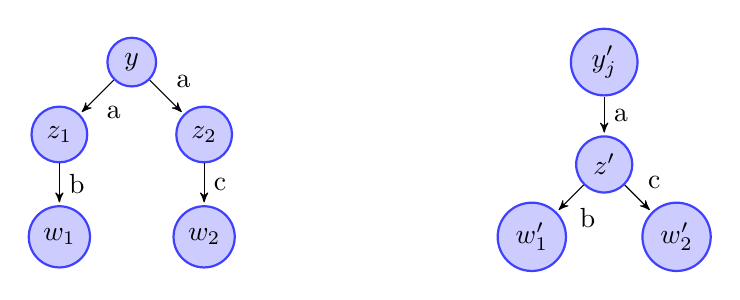
\begin{tikzpicture}[node distance=1.3cm,>=stealth',bend angle=45,auto]
  \tikzstyle{place}=[circle,thick,draw=blue!75,fill=blue!20,minimum size=6mm]
  \tikzstyle{red place}=[place,draw=red!75,fill=red!20]
  \tikzstyle{transition}=[rectangle,thick,draw=black!75,
  			  fill=black!20,minimum size=4mm]
  \tikzstyle{every label}=[red]

  \begin{scope}[xshift=0cm]
    \node [place] (t) {$y$};
    \node [place] (a) [below left of=t] {$z_1$}
      edge [pre]  node[swap] {a}                 (t);
    \node [place] (a2) [below right of=t] {$z_2$}
      edge [pre]  node[swap] {a}                 (t);
    \node [place] (b) [below of=a] {$w_1$}
      edge [pre]  node[swap] {b}                 (a);
    \node [place] (c) [below of=a2] {$w_2$}
      edge [pre]  node[swap] {c}                 (a2);
  \end{scope}  
  \begin{scope}[xshift=6cm]
    \node [place] (t) {$y'_j$};
    \node [place] (a) [below of=t] {$z'$}
      edge [pre]  node[swap] {a}                 (t);
    \node [place] (b) [below left of=a] {$w'_1$}
      edge [pre]  node[swap] {b}                 (a);
    \node [place] (c) [below right of=a] {$w'_2$}
      edge [pre]  node[swap] {c}                 (a);
  \end{scope}  
\end{tikzpicture}
\caption{{\small Worked Example of $\mathsf{neg}$. Note that the transition
  system on the left is non-deterministic.}}\label{figure:example:neg}
\end{figure}



\NI We continue with a worked example of $\mathsf{neg}$.  Consider
  $y$ and $y'_j$ as in Figure \ref{figure:example:neg}.  One formula
  that is true in $y'_j$ but not in $y$ is

\[
   \langle a \rangle (\langle b \rangle \top \AND \langle c \rangle \top)
\]

\NI Now:

\begin{eqnarray*}
\lefteqn{\mathsf{neg}(y, \langle a \rangle (\langle b \rangle \top \AND \langle c \rangle \top))}\qquad \qquad \qquad  \\
& = & \bigwedge\limits_{y \xrightarrow{a} z} \langle a \rangle \mathsf{neg}(z, \langle b \rangle \top \AND \langle c \rangle \top)  \\
& = & \langle a \rangle \mathsf{neg}(z_1, \langle b \rangle \top \AND \langle c \rangle \top) \AND \langle a \rangle\mathsf{neg}(z_2, \langle b \rangle \top \AND \langle c \rangle \top)  \\
& = & \langle a \rangle (\langle b \rangle \top \AND \mathsf{neg}(z_1, \langle c \rangle \top)) \AND \langle a \rangle\mathsf{neg}(z_2, \langle b \rangle \top \AND \langle c \rangle \top)  \\
& = & \langle a \rangle (\langle b \rangle \top \AND \mathsf{neg}(z_1, \langle c \rangle \top)) \AND \langle a \rangle(\mathsf{neg}(z_2, \langle b \rangle \top) \AND \langle c \rangle \top)  \\
& = & \langle a \rangle (\langle b \rangle \top \AND \fBang \{b\}) \AND \langle a \rangle(\mathsf{neg}(z_2, \langle b \rangle \top) \AND \langle c \rangle \top)  \\
& = & \langle a \rangle (\langle b \rangle \top \AND \fBang \{b\}) \AND \langle a \rangle(\fBang \{c\} \AND \langle c \rangle \top) 
\end{eqnarray*}

\NI The resulting formula is true in $y$ but not in $y'_j$.



\section{Omitted proofs}\label{app:completeness:proofs}\label{inc-appendix}

\subsection{Proof of Lemma \ref{lemmasimpl}}\label{app:decision:proofs}

If $\MMM \models \phi$ then $\MMM \MODELLEQ \SIMPL{\phi}$.

\begin{proof}
We shall show $\THEORY{\SIMPL{\phi}} \subseteq \THEORY{\MMM}$.
The desired result will then follow by applying Theorem \ref{theorem:completeLattice}.
We shall show that
\[
\text{If } \MMM \models \phi \text{ then } \THEORY{\SIMPL{\phi}} \subseteq \THEORY{\MMM}
\]
by induction on $\phi$.
In all the cases below, let $\SIMPL{\phi} = (\mathcal{L}, w)$ and let $\MMM = (\mathcal{L}', w')$.
The case where $\phi = \top$ is trivial.
Next, assume $\phi = \MAY{a} \psi$.
We know $\MMM \models \MAY{a} \psi$ and need to show that $\THEORY{\SIMPL{\MAY{a} \psi}} \subseteq \THEORY{\MMM}$.
Since $(\mathcal{L}', w') \models \MAY{a} \psi$, there is an $x'$ such that $w' \xrightarrow{a} x'$ and $(\mathcal{L}', x') \models \psi$.
Now from the definition of $\SIMPL{}$, $\SIMPL{\MAY{a} \psi}$ is a model combining $\SIMPL{\psi}$ with a new state $w$ not appearing in $\SIMPL{\psi}$ with an arrow $w \xrightarrow{a} x$ (where $x$ is the start state in $\SIMPL{\psi}$), and $\lambda(w) = \Sigma$. 
Consider any sentence $\xi$ such that $\SIMPL{\MAY{a} \psi} \models \xi$. Given the construction of $\SIMPL{\MAY{a}\psi}$, $\xi$ must be a conjunction of $\top$ and formulae of the form $\MAY{a} \tau$. In the first case, $(\mathcal{L}', x')$ satisfies $\top$; in the second case, $(\mathcal{L}', x') \models \tau$ by the induction hypothesis and hence $(\mathcal{L}', w') \models \MAY{a} \tau$.

Next, consider the case where $\phi = !A$, for some finite set $A \subset \Sigma$.
From the definition of $\SIMPL{}$, $\SIMPL{!A}$ is a model with one state $s$, no transitions, with $\lambda(s) = A$.
Now the only formulae that are true in $\SIMPL{!A}$ are conjunctions of $\top$ and $!B$, for supersets $B \supseteq A$.
If $\MMM \models !A$ then by the semantic clause for $!$, $\lambda'(w') \subseteq A$, hence $\MMM$ models all the formulae that are true in $\SIMPL{!A}$.

Finally, consider the case where $\phi = \psi_1 \land \psi_2$.
Assume $\MMM \models \psi_1$ and $\MMM \models \psi_2$.
We assume, by the induction hypothesis that $\THEORY{\SIMPL{\psi_1}} \subseteq \THEORY{\MMM}$ and $\THEORY{\SIMPL{\psi_2}} \subseteq \THEORY{\MMM}$.
We need to show that $\THEORY{\SIMPL{\psi_1\land \psi_2}} \subseteq \THEORY{\MMM}$.
By the definition of $\SIMPL{}$, $\SIMPL{\psi_1 \land \psi_2} = \SIMPL{\psi_1} \sqcap \SIMPL{\psi_2}$.
If $\SIMPL{\psi_1}$ and $\SIMPL{\psi_2}$ are $\mathsf{inconsistent}$ (see the definition of $\mathsf{inconsistent}$ in Section \ref{simpl}) then $\MMM = \bot$. In this case, $\THEORY{\SIMPL{\psi_1} \land \SIMPL{\psi_2}} \subseteq \THEORY{\bot}$.
If, on the other hand, $\SIMPL{\psi_1}$ and $\SIMPL{\psi_2}$ are not $\mathsf{inconsistent}$, we shall show that $\THEORY{\SIMPL{\psi_1 \land \psi_2}} \subseteq \THEORY{\MMM}$ by reductio.
Assume a formula $\xi$ such that $\SIMPL{\psi_1 \land \psi_2} \models \xi$ but $\MMM \nvDash \xi$.
Now $\xi \neq \top$ because all models satisfy $\top$.
$\xi$ cannot be of the form $\MAY{a} \tau$ because, by the construction of $\mathsf{merge}$ (see Section \ref{simpl}), all transitions in $\SIMPL{\psi_1 \land \psi_2}$ are transitions from $\SIMPL{\psi_1}$ or $\SIMPL{\psi_2}$ and we know from the inductive hypothesis that $\THEORY{\SIMPL{\psi_1}} \subseteq \THEORY{\MMM}$ and $\THEORY{\SIMPL{\psi_2}} \subseteq \THEORY{\MMM}$.
$\xi$ cannot be $!A$ for some $A \subset \Sigma$, because, from the construction of $\mathsf{merge}$, all state-labellings in $\SIMPL{\psi_1 \land \psi_2}$ are no more specific than the corresponding state-labellings in $\SIMPL{\psi_1}$ and $\SIMPL{\psi_2}$, and we know from the inductive hypothesis that $\THEORY{\SIMPL{\psi_1}} \subseteq \THEORY{\MMM}$ and $\THEORY{\SIMPL{\psi_2}} \subseteq \THEORY{\MMM}$.
Finally, $\xi$ cannot be $\xi_1 \land xi_2$ because the same argument applies to $xi_1$ and $xi_2$ individually.
We have exhausted the possible forms of $\xi$, so conclude that there is no formula $\xi$ such that $\SIMPL{\psi_1 \land \psi_2} \models \xi$ but $\MMM \nvDash \xi$.
Hence $\THEORY{\SIMPL{\psi_1\land \psi_2}} \subseteq \THEORY{\MMM}$.
\end{proof}


\subsection{Proof of Lemma \ref{inc1}}
If $\phi \models \psi \mbox{ then } \SIMPL{\phi} \MODELLEQ \SIMPL{\psi}$

\begin{proof}
By Theorem \ref{theorem:completeLattice}, $ \SIMPL{\phi} \MODELLEQ \SIMPL{\psi}$ iff $\THEORY{\SIMPL{\psi}} \subseteq  \THEORY{\SIMPL{\phi}}$.
Assume $\phi \models \psi$, and assume $\xi \in \THEORY{\SIMPL{\psi}} $. We must show $\xi \in \THEORY{\SIMPL{\phi}} $.
Now $\SIMPL$ is constructed so that:
\[
\SIMPL{\psi} = \bigsqcup \{ \MMM \; | \; \MMM \models \psi \}
\]
So  $\xi \in \THEORY{\SIMPL{\psi}} $ iff for all models $\MMM$, $\MMM \models \psi$ implies $\MMM \models \xi$.
We must show that $\MMM \models \phi$ implies $\MMM \models \xi$ for all models $\MMM$.
Assume $\MMM \models \phi$. Then since $\phi \models \psi$,  $\MMM \models \psi$. 
But since $\xi \in \THEORY{\SIMPL{\psi}} $, $\MMM \models \xi$ also.

\end{proof}

\subsection{Proof of Lemma \ref{inc3}}
If $\mathcal{I}(\psi) \subseteq \mathcal{I}(\phi) \mbox{ then } \mathcal{J}(\SIMPL{\psi}) \subseteq \mathcal{J}(\SIMPL{\phi})$
\begin{proof}
Assume $\mathcal{I}(\psi) \subseteq \mathcal{I}(\phi)$ and $\MMM \sqcap \SIMPL{\psi} = \bot$.
We need to show $\MMM \sqcap \SIMPL{\phi} = \bot$.
If $\mathcal{I}(\psi) \subseteq \mathcal{I}(\phi)$ then for all formulae $\xi$, if $\SIMPL{\xi} \sqcap \SIMPL{\psi} = \bot$ then $\SIMPL{\xi} \sqcap \SIMPL{\phi} = \bot$.
Let $\xi$ be $\CHAR{\MMM}$.
Given that $\MMM \sqcap \SIMPL{\psi} = \bot$ and $\SIMPL{\CHAR{\MMM}} \MODELLEQ \MMM$, $\SIMPL{\CHAR{\MMM}} \sqcap \SIMPL{\psi} = \bot$.
Then as $\mathcal{I}(\psi) \subseteq \mathcal{I}(\phi)$, $\SIMPL{\CHAR{\MMM}} \sqcap \SIMPL{\phi} = \bot$.
Now as $\MMM  \MODELLEQ \SIMPL{\CHAR{\MMM}}$, $\MMM \sqcap \SIMPL{\phi} = \bot$.

\end{proof}



\end{document}
